%Package Date: 2018-01-01 % !TeX program = XeLaTeX
\documentclass[12pt]{report} \usepackage{preamble}

\title{\textbf{\huge Vulkan Unveiled: A Beginner's Guide to Professional
Graphics Programming}} \author {Nick Schefner}
\bibliography{citations.bib}

\begin{acronym}
	\acro{API}{Application Programming Interface}
	\acro{CPU}{Central Processing Unit}
	\acro{GPU}{Graphics Processing Unit}
	\acro{VRAM}{Video Random Access Memory}
	\acro{SIMD}{Single Instruction, Multiple Data}
  \acro{GLM}{OpenGL Mathematics}
  \acro{NDC}{Normalized Device Coordinates}
  \acro{CVV}{Canonical View Volume}
  \acro{SM}{Streaming Multiprocessor}
  \acro{LOD}{Level of Detail}
  \acro{GLSL}{OpenGL Shading Language}
  \acro{Spir-V}{Standard Portable Intermediate Representation}
  \acro{UBO}{Uniform Buffer Object}
  \acro{GLFW}{Graphics Library Framework}
  \acro{MSAA}{Multisample Anti-Aliasing}
  \acro{HLSL}{High Level Shading Language}
  \acro{FBX}{Filmbox}
  \acro{glTF}{Graphics Library Transmission Format}
  \acro{OBJ}{Wavefront Object}
  \acro{UBO}{Uniform Buffer Object}
\end{acronym}

\begin{document} \maketitle

\tableofcontents

\chapter{Introduction}

Dear reader,

Welcome to "Vulkan Unveiled: A beginner's guide to professional graphics programming".
It is with great pleasure and excitement that I extend my sincerest greetings
to you as you embark on this journey into the world of the Vulkan \ac{API} .
Before we start, I would like to introduce myself to you.

I began my journey with the Vulkan \ac{API} about 9 months ago when I embarked
on the creation of my own game engine “Magma”, which is just a very basic
implementation of a game engine. Before that, I have
started my programming journey with the well known unity game engine
and learned many basics on how games and graphics behave. I also have
experience with glium, which is an OpenGL wrapper for rust. For those
unfamiliar, glium further abstracts OpenGL, which made it easier to
understand the logic and functionalities of my application.  I’m deeply
invested in creating a precise representation of the Vulkan \ac{API}.
Which will also be my ground base on further deepening my knowledge and
understanding.	While researching and writing this book, I anticipate
learning a great deal myself.  Nonetheless, I am committed to providing
you with a comprehensive understanding of graphics programming throughout
this book.

Graphical programming is a complex topic with a steep learning curve,
i often feel that I missed the dots connecting every aspect of the
underlying technologies when first getting started in this field as a
game dev. Therefore it might be quite overwhelming at first, to understand
how the graphics that we see every day are created and displayed onto
our displays. It does not help that Vulkan expands on that complexity
and provides us with an \ac{API} that is very low level, whereas older graphic
\ac{API}s abstract many of the processes, that Vulkan requires us to handle
ourself.

Because Vulkan requires us to explicitly control the hardware resources,
you need even more knowledge about the multiple hardware components and
rendering possibilities that modern \ac{GPU}s allow us to employ.

The main idea off this book is to slowly introduce someone who has had
no contact with graphical programming so far, but is excited to dive
into an interesting topic that is a must know for every aspiring future
game developer or artist. We will first learn to understand the \ac{GPU} and
its usage. I will then focus on explaining pipelines, buffers, swap chains
and other components of the render system and explain in detail how they work
and are linked together. Besides that I will explain how Vulkan manages
each of these components and give an example on how a possible implementation
could look like.

I also want to give a special thanks to Brendan Galea for his “Vulkan
(C++) game engine” series, that helped me out a lot on understanding
not just Vulkan as an \ac{API} but also the basics of graphical programming
and its components.

Lastly, I want to assure you that while learning Vulkan may seem daunting
at first, with time and patience, anyone interested in this topic can
develop a strong understanding of it.

\chapter{The GPU}

\section{Why do we need a GPU?}

The graphics processing unit (\ac{GPU}) is, like the name implies, a hardware
component that is made specifically for processing graphical data. Sure,
okay, but why do we need a separate hardware component for that?  Why not
just let the \ac{CPU} handle the calculations? The answer is simple: speed
and parallelism.

The \ac{CPU} is great at executing one command after another, but
it is not very good at executing multiple commands at the same
time. Sure we have multi threading but the \ac{CPU} is limited to just a
few cores. \cite{CDW-cpu_vs_gpu} on the other hand, the \ac{GPU} is mainly
build on processing mathematically complex operations like matrix
multiplications, that are not just executed once but multiple
times. \cite{NVIDIA-cpu-gpu} because the \ac{GPU} focuses on speed
and parallelism, it is designed to use more of the accessible
transistors for processing data. This is beneficial for parallel
computations because the \ac{GPU} can hide memory access latencies with
computation. The \ac{CPU} on the other hand has an additional cache layer
and a more complex control logic that makes sequential computations
faster. \cite{CUDA_Programming_Guide}

Imagine creating a animation where the color of your full screen changes
between red and green. In that case you have a single command, the color
change, which is performed on every pixel on the screen. Using a \ac{CPU}
we would have to wait for the \ac{CPU} to execute the command on every pixel
one after another, which would take a lot of time. With the \ac{GPU} we can
execute the command on every pixel simultaneously, which is much faster.

While a \ac{CPU} usually just has a hand full of cores, \ac{GPU}s have multiple
thousands of cores. \cite{NVIDIA-rtx-4090}
but that doesn't mean that the \ac{GPU} is 1000
times faster than the \ac{CPU}. The compute units of the \ac{GPU} are much slower
than the cores of the \ac{CPU}, but because they can run in parallel they are
more suitable for graphical computations. \cite{CUDA_Programming_Guide}

The \ac{GPU} also has its own memory called the \ac{VRAM}
which is used to store processed and unprocessed data.
I don't want to go into detail about the \ac{VRAM} because it is not relevant
for understanding Vulkan, but it is important to add that the \ac{VRAM}
allows simultaneously reading and writing data, which is a big advantage
over the \ac{CPU}. \cite{vram}

It might also be interesting that when the \ac{VRAM} is full, rendering
speed and performance will drop because we need to get the data from a
slower memory source like the DRAM.  Therefore it is important to manage
data efficiently and to not overload the \ac{VRAM} by, for example, loading
to many or to detailed textures.

\section{Basic architecture of the GPU}

I've already mentioned that the \ac{GPU} can take one instruction and
execute it on multiple threads at the same time. This is called \ac{SIMD}.
\cite{cherry_gpu_architecture}

The \ac{GPU} is made up of thousands of small cores, which are called CUDA
compute units on NVIDIA graphics cards \cite{CUDA_Programming_Guide}
and ROCM compute units on AMD graphics, which I will neglect to
simplify this topic. \cite{rocm} CUDA stands for "compute unified
device architecture" and is a low level parallel computing platform
and programming model that comes with an \ac{API} for writing programs
that can handle the power and advantages of the \ac{GPU}in a high level
language like c or C++. \cite{CUDA_Programming_Guide} don't worry, we
will not use CUDA or an assembly language in this book, because Vulkan
abstracts the usage of the \ac{GPU} for us, but it is important to understand
that the \ac{GPU} is not just a black box that we can throw commands at and
expect it to work. These cores are combined into an array of so called
\ac{SM} also known as cuda blocks, which are the
main building blocks of the \ac{GPU}.  Each \ac{SM} has its own control logic,
memory and execution units. \cite{CUDA_Programming_Guide} these sms are
then combined into a grid called the \ac{GPU}.  When the \ac{GPU} is invoked by
the \ac{CPU}, a free \ac{SM} will be assigned to performing the requested tasks
and then return the results to the \ac{CPU} if needed. \cite{CUDA_Programming_Guide}

The \ac{GPU} also consists of a memory hierarchy, which is used to store the
data that is processed by the \ac{GPU}. The memory hierarchy looks like this:

\begin{figure}[hbtp]
	\centering
	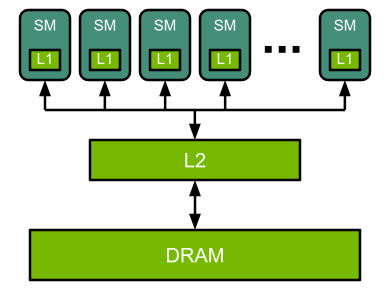
\includegraphics[width=0.70\textwidth]{simple-gpu-arch.png}
	\caption{Memory hierarchy of the \ac{GPU} \cite{fig:gpu-arch}}
\end{figure}

Please note that the VRAM is not part of the memory hierarchy, but is
connected to the L2 cache. Caches are used to store frequently used
data and to reduce access times to the main memory. While every \ac{SM}
has its own L1 cache, the L2 cache is shared between all \ac{SM}. Which
means that all cores in one \ac{SM} are sharing one L1 cache. The \ac{CPU}
on the other hand has one cache and one memory controller per
core. \cite{CUDA_Programming_Guide}

\section {Summary}

Okay that was a lot of information, so let's summarize the really
important bits of what we have learned so far.

The \ac{GPU} was created to process graphical data much faster than a \ac{CPU}
could ever do. It allows us to execute the same command on multiple
data simultaneously to prevent waiting for a single command to finish,
which helps us render reoccurring tasks like drawing a texture or model
much faster.  It is made up of many cores which are combined into an
array of \ac{SM} to allow better control and
management of the cores.  The VRAM is the memory of the \ac{GPU} and its
important to optimize your data to prevent overloading the VRAM.

\chapter{Graphics rendering pipeline}

\section{What is the graphics pipeline?}

When we talk about the graphics pipeline, I want to make clear that we
are not talking about a physical pipeline that is used to transport data
from one place to another. I've made that mistake when I first started
working with pipelines. My first thought was that the pipeline is a tool
to transport data from the \ac{CPU} to the \ac{GPU}, but that's totally wrong.

What is it then? Let's start with a simple definition.

The graphics pipeline is an abstraction layer that is located on the
\ac{GPU} and is used to process incoming data to create the image that we see
on our screen. \cite{vkGuide} this saves us from writing low level code
explicitly targeting the \ac{GPU}, which would be a massive task to do.
The name pipeline comes from the fact that we pass data through
multiple stages that process the data in a specific way. Once the data
has passed through all stages, it is ready to be displayed on the screen.

Please note that the pipeline is implemented differently in every graphics
\ac{API}, but the basic ideas remains the same. We feed the pipeline with some
graphical data, which then performs operations to transform the data into
a 2D image that can be displayed on our screen. The processed data
is then stored in a framebuffer, which will be explained later.
\cite{vkGuide}

There are other pipeline types, like the compute or ray tracing
pipeline, made for different tasks, but we will focus on the graphics
pipeline for now.

The graphics pipeline is invoked by a draw command, which starts the
data processing. \cite{build-pipeline}

\section{The basics}

To understand the graphics pipeline, we first need to understand
how the 2D image on our screen is created from the 3D data that we
provide to the pipeline.

\subsection{Vertices and Indices}

Every model that we see is made up of off either triangles, points or
isolines. These shapes are called primitives and are created by connecting
vertices so that they form the corners of the primitive. For points we
only need one vertex.
A single vertex can contain multiple attributes like position \{x, y, z\},
color \{r, g, b, a\} or texture coordinates \{u, v\}. \cite{vulkan-vertex-input}

\begin{figure}[hbtp]
	\centering \includesvg[width=0.60\textwidth]{vektor_triangle.svg}
	\caption{Triangle with vertices}
\end{figure} \Floatbarrier

When we want to reuse certain vertices, for example when
drawing a square, we can add indices.  These indices tell the
input assembler what vertices need to be combined to form a
triangle. \cite{vulkan-tutorial-index-buffer}

For example: A square has 4 vertices because it has 4 corners. When we want
to draw the square we have to create two triangles, which means we need 2 *
3 indices.

Vertices: \{0, 1, 2, 3\} Indices: \{\textcolor{red}{0, 1, 2} ,
\textcolor{blue}{0, 2, 3}\}

\begin{figure}[hbtp]
	\centering \includesvg[width=0.50\textwidth]{vi_quad.svg}
	\caption{Square
		with vertices created using indices}
\end{figure} \Floatbarrier

Here you can see that the first triangle is created by using the
vertices\{\textcolor{red}{0, 1, 2}\} and the second triangle is created by using
the vertices\{\textcolor{blue}{0, 2, 3}\}. I've added the colors just
to clarify which indices are used to create which triangles.

\subsection{Buffers}

Now that we know what vertices and indices are, we can talk about how we
provide the \ac{GPU} with this data. There the buffers come into play. A buffer
is basically an array of data that can be bind to the graphics pipeline.
When the pipeline is created, we need to provide it with the layout of the
buffer, which tells the pipeline how the data in the buffer is structured.
\cite{vulkan-tutorial-vertex-buffer}

In the vertex buffer we store the attributes of each vertex as an
array. An attribute can be a position, color or any other related data
of the vertex. \cite{vulkan-tutorial-vertex-buffer}

\begin{figure}[hbtp]
	\centering \includesvg[width=1\textwidth]{vertexbuffer.svg}
	\caption{Interleaved vertex buffer}
\end{figure} \Floatbarrier

You can see that each attribute has a specific location in the buffer.
These locations tell the pipeline what bytes belong together. So when
accessing the buffers 0st location it gets an vec3(x,y,z).  The pipeline
also needs to know by what offset, in bytes, each location is separated.
In this case it would be 12 bytes for the color, because the position
contains 3 floats, which are 4 bytes each if you use single precision
floats and 8 bytes each when you use double precision floats. \cite{vulkan-tutorial-vertex-buffer}

This example shows a single buffer containing all attributes in
an interleaved pattern, but we can also create one buffer for each
attribute and then attach them into a single vertex buffer. This is called
a non-interleaved pattern.

\begin{figure}[hbtp]
	\includesvg[width=1\textwidth]{non-int-vertexbuffer.svg}
	\caption{Non-interleaved vertex buffer}
\end{figure} \Floatbarrier

Each attribute has has its own binding, to tell the pipeline what location
is assigned to the data. So the first binding will always be the position
until you get to the next binding, which will be the color in this case.
\cite{vulkan-tutorial-vertex-buffer}

Usually we will use interleaved buffers, but in some cases, when we need
different attributes for different tasks, we can use non-interleaved
buffers.

The index buffer on the other hand is just an simple array of integers.
\cite{vulkan-tutorial-index-buffer}


\subsection{Coordinate systems}

\begin{figure}[hbtp]
	\centering 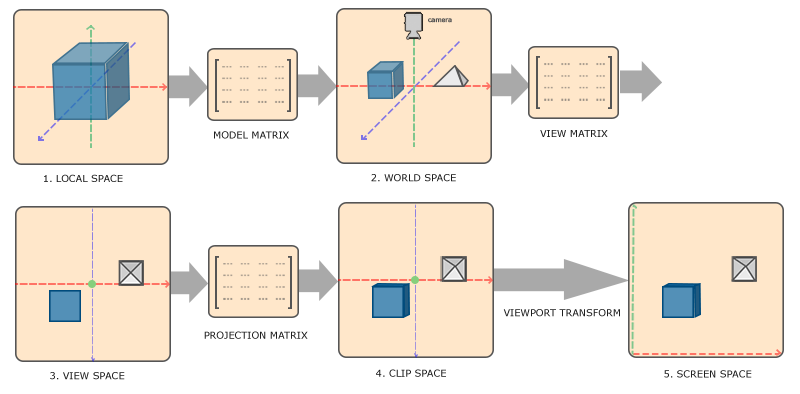
\includegraphics[width=\textwidth]{coordinate-systems.png}
	\caption{Coordinate systems \cite{fig:view-frustum}}
\end{figure}
\Floatbarrier

We start with the local space, which is the space that we use to define
our objects. Often the objects are centered around the origin of the
local space, but it is up to the modeler to decide where the object is
located. The local space is then transformed into the world space, which
is the 3D space that we use to define the positions of our objects in the scene.
The world space is then transformed into the view space, which is the space that the
camera sees. \cite{fig:view-frustum}

But wait, camera? If you have worked with 3D graphics before, you know
that we need a camera that is used to define the space we can view, aka
the view space. The camera is an object that has a view frustum
with a near and far plane, that is used to define what we can see.

\begin{figure}[hbtp]
	\centering 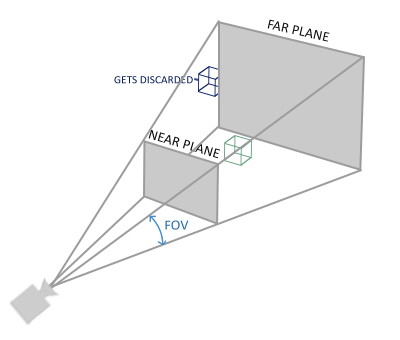
\includegraphics[width=0.60\textwidth]{view-frustum.png}
	\caption{View frustum \cite{fig:view-frustum}}
\end{figure}
\Floatbarrier

To transform the world space into the view space, we use a view matrix.
Let's briefly talk about matrix transformations and how multiplication
can be used to move, rotate or scale objects in 3D space.

If you have never touched linear algebra before, I suggest you to go over
2Blue1Brown's essence of linear algebra series on YouTube. It is a great
introduction to linear algebra and will help you understand the further topics.

\subsection{Matrix transformations}

When we have an box in 3D space, we can represent its position as an
array of 3 floats, which are the x, y and z coordinates of its center.
To move the box, we need to add or subtract a value from the x, y or
z coordinate but how can we do that? We can multiply our position with a translation matrix to
move the box. Wait how do we multiply matrices? It's simple. We multiply
the rows of the first matrix with the columns of the second matrix and add them
together. The result is the value of the new matrix at the position where the row and
column intersect.

For example, when we have two matrices a and b, we multiply them like this:

\[
	\begin{bmatrix}
		a & b & c \\
		d & e & f \\
		g & h & i \\
	\end{bmatrix}
	\cdot
	\begin{bmatrix}
		j & k & l \\
		m & n & o \\
		p & q & r \\
	\end{bmatrix}
	=
	\begin{bmatrix}
		(aj + bm + cp) & (ak + bn + cq) & (al + bo + cr) \\
		(dj + em + fp) & (dk + en + fq) & (dl + eo + fr) \\
		(gj + hm + ip) & (gk + hn + iq) & (gl + ho + ir) \\
	\end{bmatrix}
\]

\begin{figure}[hbtp]
	\centering \includesvg[width=0.60\textwidth]{images/matrix-multiplication.svg}
	\caption{Matrix multiplication \cite{fig:matrix-multiplication}}
\end{figure}
\Floatbarrier

As long as the number of columns in the first matrix is equal to the number
of rows in the second matrix, we can multiply them. The result will have
the same number of rows as the first matrix and the same number of columns
as the second matrix.

When we have a position \{x, y, z\} we cannot just move it by \{tx, ty, tz\}
because multiplying the position with the translation vector would just
multiply the coordinates. But what we need is to add the wanted translation
to the corresponding coordinate.
To do so we need to add a 4th coordinate to the position, which is called
the homogeneous coordinate. This coordinate is usually set to 1 and is used
to set the proportions of the clip space. Don't worry about the clip space
for now, we will talk about it later.

Homogeneous coordinates are used to represent the position of a point with 4
coordinates instead of 3. They have the special property that the homogeneous
coordinates are a multiple of the cartesian coordinates by the w coordinate.

So when we have a point \{1, 2, 3\} in 3D space, we can represent it as
\{1, 2, 3, 1\} in homogeneous coordinates but also as \{2, 4, 6, 2\} or
\{3, 6, 9, 3\} and so on. We will keep the w coordinate at 1, because it is
the easiest to work with.

Our position would then be \{x, y, z, 1\}. Because the w coordinate is the
fourth coordinate, we can multiply the position with a 4x4 matrix where
the forth column is the translation vector. This will add the translation
to the position as long as we keep the diagonal values of the matrix to 1,
so that we don't loose the original position in the calculation.

Therefore we can create the translation that moves the box by \{tx, ty, tz\}
like this:

\[
	\begin{bmatrix}
		1 & 0 & 0 & tx \\
		0 & 1 & 0 & ty \\
		0 & 0 & 1 & tz \\
		0 & 0 & 0 & 1  \\
	\end{bmatrix}
	\cdot
	\begin{bmatrix}
		x \\
		y \\
		z \\
		w \\
	\end{bmatrix}
	=
	\begin{bmatrix}
		x + tx*w \\
		y + ty*w \\
		z + tz*w \\
		w        \\
	\end{bmatrix}
\]

Please note that the w coordinate is changing the x, y and z coordinates,
to adjust the position to our clip space proportions.

But what if we want to rotate the box? We can't just add or
subtract a value from the boxes center to rotate it. We need to tackle each
corner of the box and move it around the center of the box.

To rotate the box, we can multiply the position of each corner with a
rotation matrix.

We can use this knowledge to create a rotation matrix. Lets say we have a line with
the points \{0, 0, 0\} and \{1, 0, 0\}.
When we want to rotate this line around an axis by \(\delta\) degrees, we can apply
the following rotation matrices to the points:

X-axis: \[
	\begin{bmatrix}
		1 & 0           & 0            & 0 \\
		0 & cos(\delta) & -sin(\delta) & 0 \\
		0 & sin(\delta) & cos(\delta)  & 0 \\
		0 & 0           & 0            & 1 \\
	\end{bmatrix}
\]

Y-axis: \[
	\begin{bmatrix}
		cos(\delta)  & 0 & sin(\delta) & 0 \\
		0            & 1 & 0           & 0 \\
		-sin(\delta) & 0 & cos(\delta) & 0 \\
		0            & 0 & 0           & 1 \\
	\end{bmatrix}
\]

Z-axis: \[
	\begin{bmatrix}
		cos(\delta) & -sin(\delta) & 0 & 0 \\
		sin(\delta) & cos(\delta)  & 0 & 0 \\
		0           & 0            & 1 & 0 \\
		0           & 0            & 0 & 1 \\
	\end{bmatrix}
\]

Let's rotate the line around the y axis:

\[
	P1 =
	\begin{bmatrix}
		cos(\delta)  & 0 & sin(\delta) & 0 \\
		0            & 1 & 0           & 0 \\
		-sin(\delta) & 0 & cos(\delta) & 0 \\
		0            & 0 & 0           & 1 \\
	\end{bmatrix}
	\cdot
	\begin{bmatrix}
		0 \\
		0 \\
		0 \\
		1 \\
	\end{bmatrix}
	=
	\begin{bmatrix}
		0 \\
		0 \\
		0 \\
		1 \\
	\end{bmatrix}
\]

\[
	P2 =
	\begin{bmatrix}
		cos(\delta)  & 0 & sin(\delta) & 0 \\
		0            & 1 & 0           & 0 \\
		-sin(\delta) & 0 & cos(\delta) & 0 \\
		0            & 0 & 0           & 1 \\
	\end{bmatrix}
	\cdot
	\begin{bmatrix}
		1 \\
		0 \\
		0 \\
		1 \\
	\end{bmatrix}
	=
	\begin{bmatrix}
		cos(\delta)  \\
		0            \\
		-sin(\delta) \\
		1            \\
	\end{bmatrix}
\]

You can see that the origin \(P1\) of the line stays the same, but the end point \(P2\)
of the line has changed. This is because we actually rotate the entire
world space and not the object itself. But because the object is in the
world space, it will also be rotated.

Scaling an object is a bit simpler than rotation. We just multiply
the position of the object with a scaling matrix that
looks like this:

\[
	\begin{bmatrix}
		s_x & 0   & 0   & 0 \\
		0   & s_y & 0   & 0 \\
		0   & 0   & s_z & 0 \\
		0   & 0   & 0   & 1 \\
	\end{bmatrix}
\]

You might see that we simply multiply the x, y and z coordinates with the
scaling factor we want to apply to that axis. So when we want to scale an
object by 2 on the x axis, we would multiply the x coordinate with 2 and
leave the y and z coordinates as they are.

A thing that is important to note is that when applying transformations,
we apply them to the entire world space. This means when rotating, scaling or
moving an object, we are actually rotating, scaling or moving the entire world,
which will also rotate, scale or move the object.

\subsection{View space}

Now that we know how to transform the world space, we can move the camera
and the objects, so that the camera is the origin of the view space.

To do so we simply take the position of the camera, for example \{1, 2, 3, 1\},
and subtract it from every object in the world space. This will move the
camera to the origin of the view space and keep the objects in the same
position relative to the camera.

\[
	\begin{bmatrix}
		1 & 0 & 0 & -1 \\
		0 & 1 & 0 & -2 \\
		0 & 0 & 1 & -3 \\
		0 & 0 & 0 & 1  \\
	\end{bmatrix}
	\begin{bmatrix}
		x \\
		y \\
		z \\
		w \\
	\end{bmatrix}
	=
	\begin{bmatrix}
		x - 1*w \\
		y - 2*w \\
		z - 3*w \\
		w       \\
	\end{bmatrix}
\]

Now that the camera is the origin of the view space, we need to rotate everything,
so that the camera is looking down the z axis. Lets say we have a camera that
is looking down this direction: \{x,y,z\}. We can create a rotation matrix that
rotates the world space so that the camera is looking down the z axis \{0, 0, z\}.

But first we need to get the angles of the rotation. We can do this by using the
dot product of the camera direction and the z axis. The dot product is simply the
cosine of the angle between two vectors. So when we have two vectors \{x, y, z\}
and \{0, 0, z\}, we can calculate the angle between them by using the dot product.

The dot product looks like this:
\[a \cdot b = |a| * |b| * cos(\theta)\]
\[a \cdot b = a_x * b_x + a_y * b_y + a_z * b_z\]

From here we can divide everything by \(|a| * |b|\) to get \(cos(\theta)= \frac{a \cdot b}{|a| * |b|}\).
Let's calculate the angles we need to rotate the camera to look down the z axis.

We start off by rotating the camera, so that it is looking down the xz plane.
This means that the y coordinate of the camera direction is 0. By taking the dot
product of the camera direction and the x axis on the same hight, we can calculate the angle
we need to rotate the camera around the z axis.

\[
	\begin{bmatrix}
		x \\
		y \\
	\end{bmatrix}
	\cdot
	\begin{bmatrix}
		1 \\
		0 \\
	\end{bmatrix}
	=
	\frac{x}{\sqrt{x^2 + y^2}}
	=
	cos(\theta)
\]

Now we just need to rotate the xz-plane around the y axis, so that the camera is looking
up the z axis. We can calculate the angle by taking the dot product of the camera direction
after rotating it around the z axis and the z axis itself

\[
	\begin{bmatrix}
		x \\
		z \\
	\end{bmatrix}
	\cdot
	\begin{bmatrix}
		0 \\
		1 \\
	\end{bmatrix}
	=
	\frac{z}{\sqrt{x^2 + z^2}}
	=
	cos(\theta)
\]

Luckily we don't need to calculate the angles by hand, we can use the
\ac{GLM} library to calculate the rotation matrix for us. The \ac{GLM} library is a
header only library that provides us with many useful functions for
mathematical operations.

Don't forget to perform all of this for every object in the world space.
The result will be the view space, where the camera is the origin and
the objects are rotated so that the camera is looking down the z axis.

\subsection{Projection transformation}

The next step is the transformation from the view space to the clip
space. The clip space is used to define what we can see
on the screen, by clipping everything that is outside of the view frustum.

This task involves transforming the view frustum into an orthographic view
volume, which is a cube with the size of the near plane and the same depth
as the frustum. Then we move the orthographic view volume to the origin
and scale it to the size of the clip space, which is plus and minus the
w coordinate on all axes. The w coordinate is almost always set to 1 by the user,
so the clip space is a cube with the length of 2 on all axes except the z axis,
because the negative z axis is behind the camera we just have the positive
z axis.

Let's start with the transformation of the view frustum to the orthographic
view volume. We basically need to scale the objects so that the far plane is
the same size as the near plane. Normally the near plane is 0.1 units away and the far
plane is 100 units away but that's up to the user to decide.

When we're looking at the frustum from the side, we can see that the camera and
the far plane create a triangle that can be divided into two right triangles at the
z axis.

\begin{figure}[hbtp]
	\centering \includesvg[width=0.80\textwidth]{images/perspective.svg}
	\caption{view frustum}
\end{figure} \Floatbarrier

What we need to calculate is yn, which is the new height of the object.
To do so we use the green triangle and the near planes distance on the z axis
(n) to get the following formula:

\[
	\frac{yn}{n} = \frac{y}{z}
\]

We can use this because the triangles sin angle is the same in the green triangle.
When we solve this for yn, we get:

\[
	yn = \frac{y * n}{z}
\]

The same can be applied for the x axis aka the width of the object:

\[
	xn = \frac{x * n}{z}
\]

The z axis stays the same.

So when we have a point \{x, y, z\} in the view space, we need to transform it to \\
\(\{\frac{x * n}{z}, \frac{y * n}{z}, z\}\) to get the orthographic view volume. Unfortunately
there is no way we can divide the x and y value with z with just 3 dimensions.
Here the w coordinate saves us again.

We transfer the z coordinate to the w variable.
This will allow us to divide the x, y and z coordinate by the z coordinate.
So what we want is to transform the point \{x, y, z, w\} to \(\{x * n, y * n, z^2, z\}\).
Keep in mind that the homogeneous coordinate is the same as the 3D coordinate after dividing by w.
This division is called the perspective divide.
So after the perspective divide we get \(\{\frac{x * n}{z}, \frac{y * n}{z}, z\}\) which are
called \ac{NDC} or the \ac{CVV}.

Okay so what we need is a 4x4 matrix that multiplies the x and y coordinate with n and the z coordinate
with itself. We also need to multiply the w coordinate with z,
to move the z coordinate to the w coordinate. This works because
w is like a scaling factor for the x, y and z coordinate but is often set to 1.

\[
	\begin{bmatrix}
		n & 0 & 0   & 0   \\
		0 & n & 0   & 0   \\
		0 & 0 & m_1 & m_2 \\
		0 & 0 & 1   & 0   \\
	\end{bmatrix}
	\begin{bmatrix}
		x \\
		y \\
		z \\
		w \\
	\end{bmatrix}
	=
	\begin{bmatrix}
		x * n \\
		y * n \\
		z^2   \\
		z     \\
	\end{bmatrix}
\]

Okay we have one last problem. How do we get to \(z^2\) ?
First we have the equation \(z^2 = m_1 * z + m_2\), considering w is 1.
The problem is that there are 2 possible solutions for m1 and m2, which we
can not work with. So we need to add 2 constrains to the equation.
We can just say that we want to apply this equation to the near and far planes z coordinate.
So we will say z = n and z = f. This will give us 2 equations that we can solve for m1 and m2.

\[
	\begin{bmatrix}
		n^2 \\
		f^2 \\
	\end{bmatrix}
	=
	\begin{bmatrix}
		m_1 * n + m_2 \\
		m_1 * f + m_2 \\
	\end{bmatrix}
\]

With this we can now calculate m1 and m2.

\[
	\begin{aligned}
		 & n^2 = m_1 * n + m_2           \\
		 & m_2 = n^2 - m_1 * n           \\
		 & f^2 = m_1 * f + m_2           \\
		 & f^2 = m_1 * f + n^2 - m_1 * n \\
		 & f^2 - n^2 = m_1 * f - m_1 * n \\
		 & f^2 - n^2 = m_1 * (f - n)     \\
		 & m_1 = \frac{f^2 - n^2}{f - n} \\
		 & m_1 = f + n                   \\
		 & m_2 = n^2 - (f + n) * n       \\
		 & m_2 = n^2 - f * n - n^2       \\
		 & m_2 = -f * n
	\end{aligned}
\]

One thing that has to be looked out for is that the near plane and far plane
are not the same because that would result in a division by zero. Also we don't
want the near plane to be 0 because that would result in weird behavior and clipping
into other objects.

Therefor the final matrix looks like this:

\[
	\begin{bmatrix}
		n & 0 & 0     & 0      \\
		0 & n & 0     & 0      \\
		0 & 0 & f + n & -f * n \\
		0 & 0 & 1     & 0      \\
	\end{bmatrix}
\]

This matrix will actually only give us \(z^2\) on the near and far plane. The objects in between will have
a little offset on the z axis but will remain linearly interpolated between the near and far plane.

Now that we have the orthographic view volume, we need to move it to the origin and
scale it to the size of the \ac{CVV}. The \ac{CVV} looks like this from the front:

\begin{figure}[hbtp]
	\centering \includesvg[width=0.60\textwidth]{images/clip-space.svg}
	\caption{\ac{CVV} front}
\end{figure} \Floatbarrier

It is a coordinate system where the y axis is pointing downwards and the positive of the z axis
is pointing away from us. Each axis ranges from -1 to 1 except the z axis,
which ranges from 0 to 1. This is because the everything negative on the z axis
is behind us and therefor not visible.

Lets first move the orthographic view volumes near planes center to the origin.

\[
	\begin{bmatrix}
		1 & 0 & 0 & -c_x \\
		0 & 1 & 0 & -c_y \\
		0 & 0 & 1 & -c_z \\
		0 & 0 & 0 & 1    \\
	\end{bmatrix}
\]


When the near plane is 0.1 units away, we need to move the orthographic view volume
by 0.1 units on the z axis. So the \(c_z\) value is the distance of the near
plane on the z axis aka n.

For the x and y value we just have to calculate the center of the near plane.
This is done by adding the opposite sides together and then dividing them by 2.
So for \(c_x\) we get \(\frac{l + r}{2}\) and for \(c_y\) we get \(\frac{t + b}{2}\).

Next we scale the orthographic view volume to the size of the \ac{CVV}.
This is done by multiplying the x, y and z coordinate
with the dimension of the \ac{CVV} over the size of the orthographic view volume.
We can get the size from subtracting the right side from the left side for the x axis,
the top from the bottom for the y axis and the far from the near plane for the z axis.
So the scaling matrix looks like this:

\[
	\begin{bmatrix}
		\frac{2}{r - l} & 0               & 0               & 0 \\
		0               & \frac{2}{t - b} & 0               & 0 \\
		0               & 0               & \frac{1}{f - n} & 0 \\
		0               & 0               & 0               & 1 \\
	\end{bmatrix}
\]

Now we can combine both transformations to get the orthographic projection matrix:

\[
	\begin{bmatrix}
		1 & 0 & 0 & -\frac{l + r}{2} \\
		0 & 1 & 0 & -\frac{t + b}{2} \\
		0 & 0 & 1 & -n               \\
		0 & 0 & 0 & 1                \\
	\end{bmatrix}
	\cdot
	\begin{bmatrix}
		\frac{2}{r - l} & 0               & 0               & 0 \\
		0               & \frac{2}{t - b} & 0               & 0 \\
		0               & 0               & \frac{1}{f - n} & 0 \\
		0               & 0               & 0               & 1 \\
	\end{bmatrix}
	=
	\begin{bmatrix}
		\frac{2}{r - l} & 0               & 0               & -\frac{l + r}{r - l} \\
		0               & \frac{2}{t - b} & 0               & -\frac{t + b}{b - t} \\
		0               & 0               & \frac{1}{f - n} & -\frac{n}{f - n}     \\
		0               & 0               & 0               & 1                    \\
	\end{bmatrix}
\]

Now we have to combine the orthographic projection matrix with the perspective projection matrix
to get the final projection matrix.

\[

	\begin{bmatrix}
		\frac{2}{r - l} & 0               & 0               & -\frac{l + r}{r - l} \\
		0               & \frac{2}{t - b} & 0               & -\frac{t + b}{b - t} \\
		0               & 0               & \frac{1}{f - n} & -\frac{n}{f - n}     \\
		0               & 0               & 0               & 1                    \\
	\end{bmatrix}
	\cdot
	\begin{bmatrix}
		n & 0 & 0     & 0      \\
		0 & n & 0     & 0      \\
		0 & 0 & f + n & -f * n \\
		0 & 0 & 1     & 0      \\
	\end{bmatrix}
	=
	\begin{bmatrix}
		\frac{2n}{r - l} & 0                & -\frac{l + r}{r - l} & 0                    \\
		0                & \frac{2n}{t - b} & -\frac{t + b}{b - t} & 0                    \\
		0                & 0                & \frac{f}{f - n}      & -\frac{f * n}{f - n} \\
		0                & 0                & 1                    & 0                    \\
	\end{bmatrix}
\]

Considering that we are looking though the center of the view frustum, we can
simplify the projection matrix to this:

r = -l, b = -t \\
\rightarrow r + l = 0, t + b  = 0 \\
\rightarrow r - l = 2r, t - b = 2t

\[
	\begin{bmatrix}
		\frac{n}{r} & 0           & 0               & 0                    \\
		0           & \frac{n}{t} & 0               & 0                    \\
		0           & 0           & \frac{f}{f - n} & -\frac{f * n}{f - n} \\
		0           & 0           & 1               & 0                    \\
	\end{bmatrix}
\]

If we now know the aspect ration of the screen and the field of view, we can calculate the top right corner of the view frustums near plane
with some trigonometry. The aspect ratio is the width of the screen divided by the height of the screen and the field of view is the angle
between the top and bottom of the view frustums near plane from the camera.

When we imagine a triangle by creating lines from the camera to the centre, with the length of n,
and to the top centre of the view frustum, we can calculate the top of the near plane with
the tangent of the FOV divided by 2, times the near plane distance.

\[
	\frac{t}{n} = tan(\frac{fov}{2}) | \cdot n
\]
\[
	t = tan(\frac{fov}{2}) * n
\]

For the right side we can use the aspect ratio and the top of the near plane to calculate the right side.

\[
	\frac{r}{t} = aspect | \cdot t
\]
\[
	r = aspect * t
\]
\[
	r = aspect * tan(\frac{fov}{2}) * n
\]

So the full perspective projection matrix can be calculated like this:

\[
	\begin{bmatrix}
		\frac{1}{aspect * tan(\frac{fov}{2})} & 0                            & 0               & 0                    \\
		0                                     & \frac{1}{tan(\frac{fov}{2})} & 0               & 0                    \\
		0                                     & 0                            & \frac{f}{f - n} & -\frac{f * n}{f - n} \\
		0                                     & 0                            & 1               & 0                    \\
	\end{bmatrix}
\]

This is the projection matrix that is used to transform the view space to the clip space
by first transforming the view frustum to a quadratic view volume and then moving and scaling
it to the proportions of the clip space. The clip space is then used to determine what is visible on the screen and what is not.
Everything that is visible will now be projected onto the 2D screen.

\subsection{Viewport transformation}

The viewport is the area on the screen where the image is displayed.
It is defined by the x and y position, the width and height and the
min and max depth and starts at the top left corner of the screen.
The viewport transformation is used to transform the \ac{NDC} to the screen space.
This is done by scaling the x and y coordinate to the width and height of the viewport,
scaling and moving the z coordinate to the depth range and then adding
half of the width to the x coordinate and subtracting half of the height from the y coordinate
to move the origin to the top left corner of the screen.

\[
	\begin{bmatrix}
		\frac{width}{2} & 0                & 0                   & \frac{width}{2}  \\
		0               & \frac{height}{2} & 0                   & \frac{height}{2} \\
		0               & 0                & maxdepth - mindepth & mindepth         \\
		0               & 0                & 0                   & 1                \\
	\end{bmatrix}
\]

This will transform the \ac{NDC} to the screen space, but we can also add an x
and y offset to the viewport to move the image around on the screen.
That would mean we need to add the x and y offset when moving
the origin to the top left corner of the screen.

\[
	\begin{bmatrix}
		\frac{width}{2} & 0                & 0                   & \frac{width}{2} + x  \\
		0               & \frac{height}{2} & 0                   & \frac{height}{2} + y \\
		0               & 0                & maxdepth - mindepth & mindepth             \\
		0               & 0                & 0                   & 1                    \\
	\end{bmatrix}
\]

Wow that was a lot of complicated math, but it's important to understand how the world is
projected onto our screen. That's the whole point of 3D graphics after all :p

Don't worry tho if you don't quite understand everything, maybe dive into some other resources to further
understand this topic and until then, do what programmers do best. Copy and paste it from somewhere else.

\section{Stages of the pipeline}

The Vulkan pipeline consists of multiple stages. Some of them are fixed
and can not be changed, while others are programmable to act as we
want them to. These changeable stages are called shaders and are usually
written in the \ac{GLSL}. Optionally it is possible
to use other shading languages like the \ac{HLSL}.
These shaders have to be given to the pipeline as compiled \ac{Spir-V} bytecode. \cite{spirv}

Lets take a look at the Vulkan pipeline and its stages:

\begin{figure}[hbtp]
	\fontsize{6}{10}\selectfont
	\centering \includesvg[width=1\textwidth]{images/pipeline.svg}
	\caption{Pipeline structure \cite{fig:pipeline}}
\end{figure} \Floatbarrier

Okay okay, I know that's a lot and there is stuff I haven't talked about
yet, like these buffers, images and the push constants. Don't worry i
will explain all of these things when going over the stages.

On the left side we have the graphics pipeline and on the right side the
compute pipeline. Now it makes sense that there are different pipelines
for different tasks, right? If we would use the graphics pipeline but
actually just need one shader to edit some data, we would waste a lot
of resources and time sending it though the graphics pipeline.

I'm going to focus on the graphics pipeline and its most important stages.
So some stages will be cut short to better explain the important ones.
In the end you will rarely need to use geometry shaders or tessellation
shaders, but it is important to know that they exist and what they do.

\subsection{Draw}

The draw "stage" is not really a stage, but the command that starts
the rendering process. When we call the vkCmdDraw command on the \ac{GPU},
the pipeline will start processing the data that we have given to
it. \cite{vulkan-spec-draw}

The vkCmdDraw command is part of the command buffer, which is used to
record and execute commands on the \ac{GPU}. This command buffer is then
submitted to a vkQueue, which will execute the commands on the \ac{GPU}
in the order they were recorded. \cite{command-buffers}

\subsection{Input Assembler}

The input assembler is the first stage of the graphics pipeline. It takes
a vertex and index buffer. \cite{vulkan-spec-pipelines}

Okay we can now finally talk about the input assembler. The input
assembler takes the vertices and indices to create primitives types like
points, lines or triangles. \cite{microsoft-ia}

\newpage

\begin{lstlisting}[Language=C++] 

  // Provided by VK_VERSION_1_0
  enum VkPrimitiveTopology {
    VK_PRIMITIVE_TOPOLOGY_POINT_LIST = 0,
    VK_PRIMITIVE_TOPOLOGY_LINE_LIST = 1,
    VK_PRIMITIVE_TOPOLOGY_LINE_STRIP = 2,
    VK_PRIMITIVE_TOPOLOGY_TRIANGLE_LIST = 3,
    VK_PRIMITIVE_TOPOLOGY_TRIANGLE_STRIP = 4,
    VK_PRIMITIVE_TOPOLOGY_TRIANGLE_FAN = 5,
    VK_PRIMITIVE_TOPOLOGY_LINE_LIST_WITH_ADJACENCY = 6,
    VK_PRIMITIVE_TOPOLOGY_LINE_STRIP_WITH_ADJACENCY = 7,
    VK_PRIMITIVE_TOPOLOGY_TRIANGLE_LIST_WITH_ADJACENCY = 8,
    VK_PRIMITIVE_TOPOLOGY_TRIANGLE_STRIP_WITH_ADJACENCY = 9,
    VK_PRIMITIVE_TOPOLOGY_PATCH_LIST = 10,
  } VkPrimitiveTopology; 
  \end{lstlisting} \cite{vulkan-spec-primitive-topology}

These are the primitive topology types that the input assembler can
create in Vulkan.  We have to tell the input assembler what type of
topology we want to create, which is usually a triangle strip or list,
but we can also create points or lines.  The difference between a list
and a strip is simple. A list will create a triangle for every 3 indices,
while a strip will create a triangle for every 3 indices and then use
the last 2 vertices of the last triangle to create the next triangle.
The same idea works with lines. The "with adjacency" types are only
used when accessing the geometry stage. We will rarely use
the adjacency types, so don't worry on understanding them now. \cite{vulkan-spec-primitive-topology}

\subsection{Vertex Shader}

The vertex shader is the first programmable stage of the pipeline.
Here we transform the world to our clip space. The vertex shader takes
the vertex data from the input assembler and transforms each vertex
to it's clip space position. \cite{vulkan-tutorial-shader-modules}

But we need to program the transformation ourselves. We can use our new
knowledge of matrices to transform the vertices. To do so we pass the
model, view and projection matrix to the vertex shader via resource descriptors.

When we want to pass data during the rendering process to the shaders,
we have to use resource descriptors. There are multiple types of descriptors, but we will
focus on the \ac{UBO} which passes data to the shaders
in the form of a buffer.

But first we have to create a descriptor layout that tells the pipeline
what type of data we are passing to which shader. Then we create a descriptor
pool that holds multiple descriptor sets. The descriptor sets are used to
bind the buffers to the shaders and are created from the descriptor pool. \cite{vulkan-tutorial-descriptors}

Descriptors are good to pass constant data to the shaders, but when we
want to pass data that changes frequently we can use push constants.
Push constants are a small amount of data that is stored in the command
buffer. We can assign a minimum of 128 bytes to the push constants, which
is enough to pass 2 4x4 matrices to the shaders. \cite{push-constants}

After that the pipeline performs the perspective divide and returns the
\ac{NDC}.

\subsection{Tessellation}

The tessellation stage is actually divided in 3 stages. The tessellation
control shader, tessellation primitive generator (Tessellator) and the tessellation
evaluation shader. Please note that the tessellation stage is optional and will
only be executed if both shaders are defined in the pipeline.\cite{tessellation}

If you are not familiar with tessellation, it is a technique used to
subdivide a polygon, a shape, into smaller polygons without leaving
any gaps in between. This can be used to create more detailed models
without having to pass all the vertex data from the \ac{CPU} to the \ac{GPU}. \cite{tessellation}

The tessellation control shader is used to define how many times
our primitive should be subdivided, by defining inner and outer tessellation levels.
It also passes the vertex positions to the evaluation shader. \cite{tessellation}

After setting the tessellation levels, the tessellator subdivides a patch, which is
a new primitive type, into smaller patches.
This can be done in 3 ways: triangles, quads or isolines.
Let's first talk about the tessellation of a triangle.

Vulkan uses barycentric coordinates to subdivide the triangle. Barycentric
coordinates consist, in the case of a triangle, of three variables (u,v,w) that sum up to 1.
Each variable represents the relative position of a vertex in the triangle with 1 being directly
on the vertex. So when we have a triangle with vertices a, b and c, the barycentric coordinates
could be \{0, 0, 1\} for a, \{0, 1, 0\} for b and \{1, 0, 0\} for c, depending on the selected
origin of the triangle. \cite{tessellation}

A point in the triangle ABC, like the center, could be calculated like this:

\[
	\begin{bmatrix}
		1 \\
		1 \\
		1 \\
	\end{bmatrix}
	\div
	3
	=
	\begin{bmatrix}
		\frac{1}{3} \\
		\frac{1}{3} \\
		\frac{1}{3} \\
	\end{bmatrix}
\]

Because the center is equally distant from all vertices,
the barycentric coordinates need to be equal for u, v and w
and when we sum them up they need to equal 1.

First the inner tessellation levels subdivides the patches edges into the desired amount of segments and
creates temporary vertices on the edges of the patch. These vertices are then used to create an
inner triangle by taking the two neighboring vertices of the outer triangles corners and extending perpendicular
lines to the edge of the outer triangle. Where these two lines intersect, a new vertex is created. When you
do this for all three corners it creates the corners of the inner triangle. \cite{tessellation}

\begin{figure}[hbtp]
	\centering 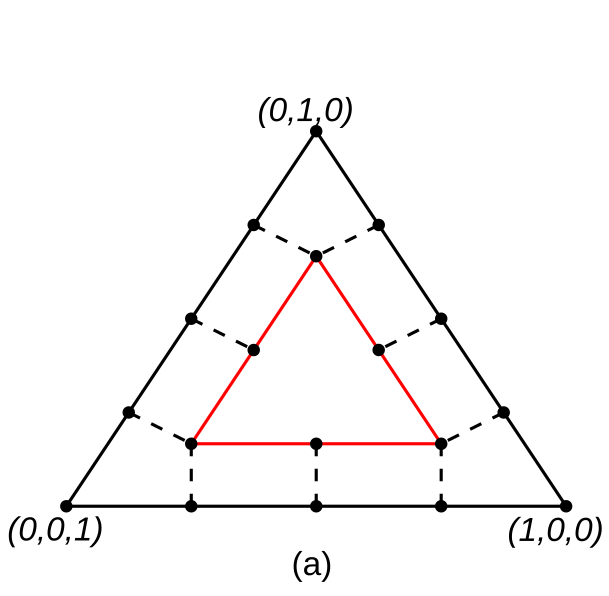
\includegraphics[width=0.4\textwidth]{innertri.png}
	\caption{Inner tessellation with 4 segments}
	\cite{fig:inner-tessellation}
\end{figure} \Floatbarrier

You can see that the inner tessellation level of four cuts each edge of the outer triangle into four segments.
This is done by calculating the barycentric coordinates of the temporary vertices on the edges. Let's
calculate the barycentric coordinates of the first vertex on the left edge ab.

We need three points where u is always zero because the vertices are on the opposite edge of the corner {1,0,0}
to get the distance of one segment we divide the edge length by the desired segments length.

So the length of one segment is \(\frac{1}{4}\).
For the first vertex we then get \{0, \(\frac{1}{4}\), \(\frac{3}{4}\}\), for the second
vertex \{0, \(\frac{2}{4}\), \(\frac{2}{4}\}\) and for the third vertex \{0, \(\frac{3}{4}\), \(\frac{1}{4}\}\).

We do the same for each edge and then calculate the intersection of the
perpendicular lines to get the inner triangles corner vertices.

For the bottom left corner of the inner triangle we take the
two vertices of the outer triangle \{0, \(\frac{1}{4}\), \(\frac{3}{4}\}\)
and \{\(\frac{1}{4}\), 0, \(\frac{3}{4}\}\).

Now we need to get the direction of the perpendicular line.
This is way easier than it sounds, because our barycentric triangle is equilateral.
That means that when we draw a line to display the height of the triangle and take it's direction,
we get the direction of the perpendicular line to the lower edge.
Luckily, because the triangle stays the same no matter how we rotate it, we can just use
the direction of the height line to get the direction of the
perpendicular lines for each triangle. \cite{equilateral-triangle}

\begin{figure}[htbp]
	\centering \includegraphics[width=0.7\textwidth]{equiletral-triangle.png}
	\caption{Equilateral triangle}
	\cite{equilateral-triangle}
\end{figure} \Floatbarrier

Considering that we can calculate the direction of the perpendicular line:

\[
	\begin{aligned}
		 & E(\frac{1}{2}, 0, \frac{1}{2})                                                      \\
		 & A(0, 1, 0)                                                                          \\
		 & A - E = (0 - \frac{1}{2}, 1 - 0, 0 - \frac{1}{2}) = (-\frac{1}{2}, 1, -\frac{1}{2}) \\
	\end{aligned}
\]

We can now add this direction to the vertex \(\{\frac{1}{4}, 0, \frac{3}{4}\}\)
to get the perpendicular lines function.

\[
	f(v) = \{\frac{1}{4} - \frac{1}{2}v, 0 + v, \frac{3}{4} - \frac{1}{2}v\}
\]

It's the same for the other points, but we need to change the direction of the perpendicular line.

\[
	f(u) = \{0+u, \frac{1}{4} - \frac{1}{2}u, \frac{3}{4} - \frac{1}{2}u\}
\]

To get the intersection we simply set the functions equal to each other and solve it.

\[
	\begin{aligned}
		     &               & f(v)= f(u)                                                                                \\
		I)   &               & \frac{1}{4} - \frac{1}{2}\cdot v & = u                                                    \\
		II)  &               & v                                & = \frac{1}{4} - \frac{1}{2}\cdot u                     \\
		III) &               & \frac{3}{4} -\frac{1}{2}\cdot v  & = \frac{3}{4} -\frac{1}{2}\cdot u                      \\
		     &               & v                                & = u                                                    \\
		I)   &               & \frac{1}{4} - \frac{1}{2}\cdot u & = u                                                    \\
		     &               & \frac{3}{2}\cdot u               & = \frac{1}{4}                                          \\
		u    & = \frac{1}{6} & v                                & = \frac{1}{6}                      & w & = \frac{4}{6}
	\end{aligned}
\]

Voil\`a, that's how we get the corners of the inner triangle.
Now Vulkan subdivides the inner triangles edges by n-2 with n being the
inner tessellation level. Because our tessellation level is 4
we subdivide the first inner triangles edges into 2 pieces.
The vertex dividing the inner edge is then calculated by projecting a
perpendicular line from the outer edge to the inner edge.
We repeat this until n is smaller than 3, but when we start with n = 2
we will have a tessellation vertex in the center of the triangle. \cite{tessellation}

When we have calculated all inner tessellation vertices we fill the area of the
concentric triangles with triangles by connecting the vertices in a way that
ensures that the triangles are not overlapping. If the inner tessellation level is 2 and
no outer tessellation level is set, the tessellator will connect the corners
of the triangle with the center vertex. \cite{tessellation}
unfortunately, considering more complicated tessellation, the order in which the vertices
are created and connected is implementation dependent,
which means that it is up to the \ac{GPU} to decide how the vertices are connected. \cite{tessellation}

After the inner patches are filled, we discard the outer triangles temporary vertices
and subdivide each edge by it's outer tessellation level.
The tessellator now fills the area of the outer triangle with the outermost inner triangle.
Now that all the triangles are created, the tessellation primitive generator assigns
the vertices their barycentric coordinates (u,v,w)
and passes them to the tessellation evaluation shader. \cite{tessellation}

For quads and isolines the process is similar, but the patch only has 2 barycentric coordinates.
So we can just calculate the barycentric coordinates as if we were in
an x,y coordinate system. \cite{tessellation}

Quads have 4 outer tessellation levels that subdivide the outer edges
and 2 inner tessellation levels that subdivide the area of the square
into smaller squares. The first inner tessellation level divides the columns
and the second inner tessellation level divides the rows.
At the end the tessellator fills the area of the square with triangles. \cite{tessellation}

Isolines on the other hand is a set of horizontal lines that have a length
of 1 on the u axis and are equally spaced on the v axis.
They only have 2 outer tessellation levels that define how many single lines
are created and in how many segments they are divided.

\begin{figure}[hbtp]
	\centering \includegraphics[width=0.4\textwidth]{tessellation_isoline_6_2.png}
	\caption{Isoline tessellation (6, 2)}
	\cite{fig:isoline}
\end{figure} \Floatbarrier

These were the possible tessellation types that the tessellator
can work with but there are a few more things to consider for each of them.
For example, we can change the tessellator spacing,
which defines the spacing of the outer tessellation levels.
The tessellator spacing can be either equal, fractional even or fractional odd,
which allow us to have a tessellation level of 2.5 for example. \cite{tessellation}
we can also control the vertex winding order, which defines which side of the triangle
is the front and which is the back. This is important
for culling and lighting calculations. \cite{tessellation}

Please note that all of this is already handled by Vulkan
and all we have to do is to set the tessellation levels and optionally spacing
and winding order in the tessellation control shader and pass it over
to the tessellation primitive generator. \cite{tessellation}

After the tessellator created all of the new triangles the tessellation evaluation shader
is called to transform the new vertices to the clip space.
The tessellation evaluation shader takes each barycentric coordinate
and the position of the original triangles corner vertices, that we have forwarded in
the control shader, to calculate the position of the new vertices in clip space. \cite{tessellation}

To do so we can multiply the barycentric coordinates with the corner vertices
and add them together to get the new vertex position.
For a triangle with vertices a, b and c and barycentric coordinates \{u, v, w\}
the new vertex position would be calculated like this:

\[
	\begin{aligned}
		x & = u \cdot a_x + v \cdot b_x + w \cdot c_x \\
		y & = u \cdot a_y + v \cdot b_y + w \cdot c_y \\
		z & = u \cdot a_z + v \cdot b_z + w \cdot c_z \\
	\end{aligned}
\]

After that we can transform them further, adding curvature or displacement to the vertices.
When using a square we can adjust the vertices
by using a 2D texture like a height map to displace the vertices. \cite{tessellation}

One last thing to mention is that when we use a tessellation shader
we actually skip the perspective projection in the vertex shader and
instead do it in the tessellation evaluation shader.
This is because the newly created vertices have to be projected to the clip space
along with the original vertices. \cite{tessellation}

\subsection{Geometry Shader}

The next stage is the geometry shader. The geometry shader is used to create new
primitives and is great at procedural generation of geometry.
That includes creating particles, grass or fur. It takes all the vertices of a primitive
and generates new vertices that are then combined to
either points, line strips or triangle strips.
For example, we could take a single point and create a square around it by emitting 4 new vertices.
These will then be combined to 2 triangles by the pipeline, forming a square. \cite{geometry-shader}

I will not go further into explaining the geometry shader because its
implementation is very dependent on the use case. It is enough to know
some use cases and that we basically can create new primitives with it.

\subsection{Vertex post processing}

After all of the previous stages we can do some post processing on the vertices.
This is done by the vertex post processing stage.
Here we have many sub stages that I will go over briefly.

\textbf{transform feedback} is used to capture the output of the previous stages
and store it in a feedback buffer. This can be used to
call a new draw command with the stored data. \cite{vertex-post-processing}

\textbf{Viewport swizzle} is used to change the orientation of the viewport.
For example, we can flip the y axis to display the image upside down.
To achieve this we can define the swizzle for each axis via the
\textit{VkViewportSwizzleNV} struct. \cite{vertex-post-processing}

\textbf{Flat shading} is used to color the whole primitive with one color.
This is done by calculating the color of the first vertex and then
using this color for the whole primitive. \cite{vertex-post-processing}

\textbf{Primitive clipping} is used to discard primitives that are outside of the clip space.
This is done by checking if the primitive is
completely outside of the clip space and then discarding it. \cite{vertex-post-processing}
when only a part of the primitive is outside of the clip space,
the pipeline will discard that part and create new vertices on the edge of the clip space,
where the primitive would intersects the clip space. \cite{vertex-post-processing}

Clipping is done by checking if the vertex's x, y and z coordinates
are in between -w and w or z\textunderscore min and w for z.
If they are not, the vertex is outside of the clip space and will be discarded.

\textbf{Clipping shader outputs} is used to discard the vertex output attributes
that are outside of the clip space.

\textbf{Controlling viewport w scaling} can be used to change the w coordinate of the vertex.
This can help to adjust the depth of an object.

\textbf{Coordinate transformation} is the step where our clip coordinates (x,y,z,w)
are transformed to (x,y,z) by dividing x, y and z by w.
This step is the perspective divide and provides us with
\ac{NDC} \cite{vertex-post-processing}

\textbf{Render pass transform} can be enabled to rotate the viewport on the xy plane.
This can be used to rotate the image on the screen by either 90, 180 or 270 degrees, using the
\textit{VK\textunderscore SURFACE\textunderscore TRANSFORM\textunderscore ROTATE\textunderscore
	{degree}\textunderscore BIT\textunderscore KHR} attribute. \cite{vertex-post-processing}

\textbf{Controlling the viewport} is a stage where Vulkan scales the \ac{NDC}
to the dimensions of the viewport. It is also possible to create
scissors to only render a part of the viewport.

\subsection{Rasterization}

This stage of the pipeline converts our primitives into a 2D image.
It takes our viewport and checks which pixels aka fragments are covered by the
primitives and then fills them with the color of the primitive.

Let's take a look on how this is done. Again, there are multiple primitives that can be rasterized:
points, lines and triangles.

We'll start with triangles, because they will be needed for the other types too.

The first step of rasterization is determining if the triangle is front or back facing,
which is done by checking if the area of the triangle is positive or negative.
We can calculate the area of a triangle using the following formula:

\[
	a = -\frac{1}{2} \sum_{i=0}^{n-1} (x_i \cdot y_{i\oplus 1} - x_{i\oplus 1} \cdot y_i)
\]

This probably looks confusing so let me explain it a bit further.
N is the number of vertices in our triangle, which is 3, while I is the current
vertex's index and \(\oplus\) is basically performing \( i+1\) mod n.
So when we have a triangle with vertices a, b and c the sum could look like this:

\[a_x \cdot b_y - b_x \cdot a_y + b_x \cdot c_y - c_x \cdot b_y + c_x \cdot a_y - a_x \cdot c_y\]

Or like this:

\[a_x \cdot c_y - c_x \cdot a_y + c_x \cdot b_y - b_x \cdot c_y + b_x \cdot a_y - a_x \cdot b_y\]

Depending on the order of the vertices. If your familiar with vector math you might
recognize this as the cross product of two side vectors that originate from the same vertex.
The cross product of these two vectors gives us a vector that is perpendicular to the triangle,
which can either point towards us or away from us.
This is because our 2D display can be seen as a 3D space with the z axis pointing out of the screen.

For example we can take the two vectors \(\vec{AB} = B - A\) and \(\vec{AC} = C - A\)
and calculate the cross product of them to get the normal of the triangle.

To calculate the cross product we can look at this visual representation:

\begin{figure}[hbtp]
	\centering
	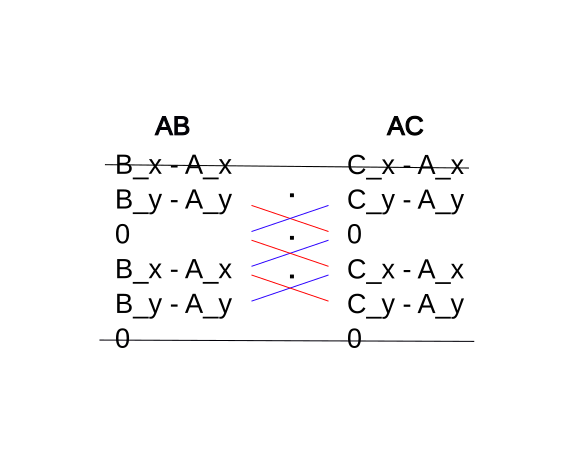
\includegraphics[width=0.5\textwidth]{cross-product.png}
	\caption{Cross product} \Floatbarrier
\end{figure}

We simply write each vector 2 times under each other, cut out the top and bottom row
and then multiply diagonally, subtract the blue result from the red result
and add each "cross" result together.

In this case we would have:

\[
	\begin{aligned}
		 & (b_y - a_y) \cdot 0 - 0 \cdot (c_x - a_x) = 0                                                                                    \\
		 & 0 \cdot (c_x - a_x) - 0 \cdot (b_x - a_x) = 0                                                                                    \\
		 & (b_x - a_x) \cdot (c_y - a_y) - (c_x - a_x) \cdot (b_y - a_y) =                                                                  \\
		 & b_x \cdot c_y - b_x \cdot a_y - a_x \cdot c_y + a_x \cdot a_y - c_x \cdot b_y + c_x \cdot a_y + a_x \cdot b_y - a_x \cdot a_y  = \\
		 & b_x \cdot c_y - b_x \cdot a_y - a_x \cdot c_y - c_x \cdot b_y + c_x \cdot a_y + a_x \cdot b_y                                    \\
	\end{aligned}
\]

This last therm comes out to our previous formula.
Now that we have a perpendicular vector to the triangle we can calculate the area of the triangle,
because the area of the triangle is half of the cross product.
That's why we multiply the cross product by \(\frac{1}{2}\).
But wait a minute, why is there a minus sign in front of the formula?
This comes from the fact that our z axis is flipped, which means that a positive area
means that the triangle is facing away from us which is not
intuitive. So we flip the sign to get a positive vector.

To actually tell the pipeline what negation is considered front facing
we can set the front face attribute in the \textit{VkPipelineRasterizationStateCreateInfo}
to either \\
\textit{VK\textunderscore FRONT\textunderscore FACE\textunderscore CLOCKWISE} or
\textit{VK\textunderscore FRONT\textunderscore FACE\textunderscore COUNTER\textunderscore CLOCKWISE}.
Clockwise means that the triangle is front facing if the area is negative
and counter clockwise then covers the opposite. \cite{rasterization}

Next they are culled according to the cull mode attribute
in the \textit{VkPipelineRasterizationStateCreateInfo}. This can be set to either
\textit{VK\textunderscore CULL\textunderscore MODE\textunderscore NONE},\\
\textit{VK\textunderscore CULL\textunderscore MODE\textunderscore FRONT},
\textit{VK\textunderscore CULL\textunderscore MODE\textunderscore BACK} or
\\
\textit{VK\textunderscore CULL\textunderscore MODE\textunderscore FRONT\textunderscore AND\textunderscore BACK}.
This determines if the front facing, back facing,
both or none of the triangles are discarded. \cite{rasterization}

Next we take the vertices of each triangle and determine its bounding box.
A bounding box is basically the smallest rectangle that
contains the whole triangle. By doing this we don't have to check every fragment
if it is inside the triangle, but only the fragments that are
inside the bounding box. This is done by taking the minimum
and maximum x and y coordinates of the triangle's vertices.

Next we iterate through every fragments center inside the bounding box,
and check if it is inside the triangle.
A point is inside the triangle if it is to the right of all
the triangles edge vectors when it is clockwise oriented
and to the left when it is counter clockwise oriented.
We can check this by calculating the cross product of the edge vectors and the vector
from the first vertex to the fragments position. If the cross product is positive
the point is to the right of the edge, if it is negative it is to the left.
If the cross product is 0 the point is on the edge.

Okay but what if the point is on an edge of adjacent triangles?
How do we know which triangle should be drawn?
For this case graphics apis usually use the top-left rule.
This rule states that left and top edges are considered to be inside the triangle
while right and bottom edges are considered to be outside. How do we know which edge is which?

A top edge is an edge where the y coordinate is flat and pointing to the right,
so where the y coordinate doesn't change
and the x coordinate is increasing when the winding order is clockwise
or else is decreasing when it is counter clockwise.

A left edge is an edge where the y coordinate is decreasing (clockwise),
which means that it is pointing upwards, because the y axis is flipped.

Is the edge a top or left edge? Then the point is inside the triangle,
otherwise an offset is added to move the point outside of the triangle.

Some of you might not like the idea of checking every fragment inside the bounding box,
because it is very inefficient. There is actually a way to rasterize
a triangle without a bounding box. To do so we have to take a look at
a fact that comes from using the barycentric coordinates.
When we go through the triangle and calculate one of the barycentric coordinates
we can see that the step size we take is always the same
when we go from one fragment in the triangle to the next.
This comes from an interesting property of the barycentric coordinates.
When we go from one fragment to the next the barycentric coordinates
change by a constant amount. This means that we can rasterize a triangle by only checking
the barycentric coordinates of the first fragment and then adding a constant amount
to the barycentric coordinates to get the barycentric coordinates.
If the barycentric coordinates are inside the triangle we draw the pixel, if not we skip it.

We can calculate the constant amount by calculating the barycentric coordinates
of the next pixel and then subtracting the barycentric coordinates
of the current fragment from them. This will give us the constant amount we have to add
to the barycentric coordinates to get the barycentric coordinates of the next fragment.

For lines and points we use the same methods, we just have to draw a box
around the line or point and then check if the fragment is inside this box.
The box drawn is not the bounding box but the thickness of the line or point.

We have two problems left.

First, lines and edges will not look smooth because we only interpolate the color of the vertices.
They will look chunky because we fully color the fragment if the center is inside the box.
To fix this we can use anti-aliasing. Anti-aliasing is a technique used to
smooth the edges of a line or point. We can do this by checking how much of the fragment
is covered by the line and then color the fragment accordingly.

Second, what if we have two triangles that overlap?
We can't just draw the second triangle over the first one.
To fix this we can use a depth buffer. You might have asked yourself why
we need a z coordinate for the vertices. This is because we can use the z coordinate
to determine which fragment is in front of each other. When we rasterize a fragment
we write the z value into an depth buffer and then we check if the z value of the next fragment is
smaller than the z value in the depth buffer. If it is we, draw the fragment and write the new depth
into the depth buffer, if not we skip it.

\subsection{Fragment Shader}

The fragment shader is the last programmable stage of the pipeline.
It takes the fragment data from the rasterization stage and performs
operations on each fragment. This is where we can calculate the color of the fragment.

To do so we need to interpolate the vertex colors.
Fortunately, we already know a way on getting the relative position
of a point to a triangles vertices, the barycentric coordinates.
We can use the barycentric coordinates to interpolate
the color of a vertex to get the color of the pixel.

But how do we get the baricentric coordinates of a pixel?
We can use the same method as before, by calculating the area of the triangle
between to vertices and the pixel. So we take the cross product of one side vector
and the vector from the first vertex to the pixel
and divide it by 2 to get its area. We do this for all 3 sides and then divide them
by the area of the full triangle to get the barycentric coordinates.

For example when we have green vertex A\{1,2\}, red vertex B\{2,3\}
and blue vertex C\{3,2\} and the coordinates of the pixel are
\{2,2.5\} we can calculate the barycentric coordinates like this:

\[
	\begin{aligned}
		\text{Area of the triangle * 2}     & = 2                                             \\
		\text{Area of the triangle ABP * 2} & = \frac{\left| 0.5 - 1 \right|}{2} = 0.25       \\
		\text{Area of the triangle BCP * 2} & = \frac{\left| (-0.5) \right|}{2} = 0.25        \\
		\text{Area of the triangle CAP * 2} & = \frac{\left| (-2) \cdot 0.5 \right|}{2} = 0.5 \\
	\end{aligned}
\]

So the barycentric coordinates are \{0.25, 0.25, 0.5\}.
If you're confused on why I'm using the area times 2, it's because we can safe the
computation of the actual area because we are only caring about
the relative position of the pixel to the vertices, so as long as everything stays
at the same scale it will give us the same answer.

Next we interpolate the colors of the vertices linearly to get the color of the pixel.
This is done by multiplying the color of each vertex, which are floats in the range of 0 to 1,
with the barycentric coordinates and adding them together.

\[
	\begin{aligned}
		r & = 0.25 \cdot a_r + 0.25 \cdot b_r + 0.5 \cdot c_r  \\
		g & = 0.25 \cdot a_g + 0.25 \cdot b_g + 0.5 \cdot c_g  \\
		b & = 0.25 \cdot a_b + 0.25 \cdot b_b + 0.5 \cdot c_b  \\
		\\
		r & = 0.25 \cdot 0 + 0.25 \cdot 1 + 0.5 \cdot 0 = 0.5  \\
		g & = 0.25 \cdot 1 + 0.25 \cdot 0 + 0.5 \cdot 0 = 0.25 \\
		b & = 0.25 \cdot 0 + 0.25 \cdot 0 + 0.5 \cdot 1 = 0.25 \\
	\end{aligned}
\]

Which will give us this color: \{0.5, 0.25, 0.25\}. This will then be converted to the color
space of our surface, which can be SRGB, DisplayP3 or some other supported color space.
We repeat this for every fragment inside the triangle and then we have our rasterized image.

But we can do more than just interpolate the color of the vertices.
We can also apply lighting, textures and more.

\subsection{Blending}

The last stage of the pipeline is blending. Blending is used to create transparency
and some other graphical effects. There isn't much to say about blending.
It gives us many options to blend the color of the fragment but all of the operations are
performed by the \ac{GPU}, so we don't have to worry about it.
When blending is complete we have our final framebuffer that we can display.

\section{Drawing process}

\subsection{Framebuffers}

A framebuffer consists of multiple attachments. An attachment is the buffer
that holds either the color or depth of each fragment.
These buffers are written to by the pipeline and then presented to the screen.
The color attachment is used to store the color of each fragment,
while the depth attachment is used to store the depth of each fragment.
The depth attachment is used to save the z coordinate of each fragment to prevent
drawing over fragments if they are not visible. \cite{framebuffers}

\subsection{Render pass}

A render pass holds the information about how many color and depth attachments
we have and how they are used in the pipeline.
It can consist of multiple subpasses, which are used to render the scene in multiple steps.
For example, we can render the scene
in one subpass and then apply post processing in another subpass. \cite{render-pass}

\subsection{Swapchain}

The swapchain is used to present the final framebuffer to the screen.
It consists of usually 2 (double buffering) or more framebuffers. The best implementation
is to use triple buffering, which uses 3 framebuffers.
On a swapchain we can present one framebuffer while we render to another framebuffer.
The presented framebuffer is called the front buffer and the rendered framebuffer
is called the back buffer. Every time a new frame is rendered the
front and back buffers are swapped. This is done to prevent screen tearing.
You know when the screen is cut into 2 different images? That's screen tearing.
It happens when the \ac{GPU} is rendering to the framebuffer while the screen is reading from it.
But that only happens when we have v-sync disabled.

There are two problems with double buffering. It can cause input lag.
This is because the \ac{GPU} has to wait for the swapchain to swap the framebuffers
before it can render the next frame. To fix this we can use triple buffering.
The other problem occur when the \ac{GPU} takes longer than one frame.
This will cause the swapchain to wait for the \ac{GPU} to finish rendering the frame
before it can swap the framebuffers. This will cause the frame
to drop and the game to stutter. To fix this we can use a third buffer
to render to while the \ac{GPU} is rendering the frame. This way the \ac{GPU} can
swap the framebuffers without waiting for the \ac{GPU} to finish rendering the frame. \cite{swapchain}

\section{Conclusion}

This was a brief overview of the Vulkan pipeline and its rendering.
Now that we have a basic understanding of the pipeline we can start
programming our first Vulkan application. In the next chapter we will set up
the Vulkan environment and create a window to render to.

\chapter{Setting up Vulkan}

Because the setup of Vulkan is highly dependent on your operating system and IDE
I will only give a brief overview of the setup process.

Let's start by setting up our development environment.
First of all we need to to install the Vulkan SDK. You can download it from the
\href{https://Vulkan.lunarg.com/sdk/home}{lunarg} website or use your preferred package manager.

Now verify if your \ac{GPU} and drivers support Vulkan.
To do so go into the bin folder of the Vulkan SDK and run the
\textit{vkcube.exe} program. If it runs without any errors and display a cube you are good to go.
If not you have to update your drivers or include the Vulkan runtime in your system.

Next we'll need to install \ac{GLFW}, a library for creating windows and handling input.
We will use it to create a window for our application.
You can download the 64-bit binaries from the \href{https://www.glfw.org/download.html}{GLFW} website or
use your package manager. After downloading the binaries,
extract them to a location that is easy to access.

Because Vulkan does not include a library for
linear algebra operations we will use the \href{https://github.com/g-truc/glm}{OpenGL mathematics}
library. Again, download the library and extract it to a location that is easy to access.

Don't forget to install a C++ and \ac{GLSL} compiler when needed.

Next you will need to either setup your IDE or write a makefile to compile your program.

This is a very brief overview of the setup process,
because explaining the setup for every operating system and IDE would be too much.
Please read through this \href{https://Vulkan-tutorial.com/development_environment}{Vulkan tutorial}
to get a more detailed explanation.

\section{Creating a window}

Before we can start rendering we need to create an application window,
because Vulkan is only a graphics API and doesn't provide a way to create a window.
Do not worry about implementing a window from scratch,
because there are libraries for creating windows for Vulkan. We will use the
previously installed open source and multi-platform library \ac{GLFW},
which provides us with a simple \ac{API} that we can use to create a window and handle input. \cite{glfw}

Let's start by creating a core folder in our source folder. Here all of the core functionalities
of our game engine will be stored. In this folder create a new header file called window.hpp.

Inside we first need to include the \ac{GLFW} header file and the define of \\
\textit{GLFW\textunderscore INCLUDE\textunderscore VULKAN} to include the Vulkan header files.

\begin{lstlisting}[Language=C++]
  #define GLFW_INCLUDE_VULKAN
  #include <glfw/glfw3.h>
\end{lstlisting}

Next we add a namespace that we want to use for our engine. In my case I will use
the namespace \textit{engine}, but feel free to use the actual name of your engine.
Inside we create our class window with an constructor that takes the width, height
and name of the window as arguments. We also add a destructor to clean up the window.

\begin{lstlisting}[Language=C++]
  #include <string>
  namespace engine {
    class Window {
    public:
      Window(int width, int height, std::string name);
      ~Window();
    };
  }
\end{lstlisting}

The job of the constructor is to initialize a window with the given width, height and name.
So let's create a private helper function that initializes the window. We will call it
\textit{initWindow}. Let's also store the width, height and name of the window in private variables.
After initializing the window we will need a pointer to the window object, so we can access it later.

\begin{lstlisting}[Language=C++]
  class Window {
      public:
        Window(int width, int height, std::string name);
        ~Window();
      private:
        void initWindow();
      
        const int width;
        const int height;
      
        std::string name;
        GLFWwindow* window;
    };
\end{lstlisting}


That's the header file for now. Let's implement the defined functions in the source file.
In the window.cpp file we include the window.hpp file add the namespace and
call the \textit{initWindow} function in the constructor and set the width, height and name of the class.

\begin{lstlisting}[Language=C++]
#include "window.hpp"

namespace engine {
  Window::Window(int width, int height, std::string name)
  : width(width), height(height), name(name) {
      initWindow();
    }
}
\end{lstlisting}

Let's implement the \textit{initWindow} function. First we need to initialize \ac{GLFW} with the
\textit{glfwInit} function. Then we set two window hints with the \textit{glfwWindowHint} function.
The first hint is the \textit{GLFW\textunderscore CLIENT\textunderscore API} and we set it to
\textit{GLFW\textunderscore NO\textunderscore API}. This tells
\ac{GLFW} to not create context for the OpenGL \ac{API}, because it was originally designed for OpenGL. \cite{client-api-hint}
The second hint is called \textit{GLFW\textunderscore RESIZABLE} and will be set to \textit{GLFW\textunderscore FALSE}
for now, but will be changed later, when implementing a resizable window.

Once we're done with setting up the window we can create it with the \textit{glfwCreateWindow} function.
It takes the width, height, title as a char pointer, a \textit{GLFWmonitor} pointer, to create a full screen
window and a 5th parameter that is OpenGL specific. Pass in our variables, set the monitor pointer to a
\textit{nullptr}, making our window use windowed mode and do the same for the last parameter.

The output will be a pointer to our created \textit{GLFWwindow} that we can store in our \textit{window}
pointer.

\begin{lstlisting}[Language=C++] 
void Window::initWindow() {
  glfwInit();

  glfwWindowHint(GLFW_CLIENT_API, GLFW_NO_API);
  glfwwindowhint(GLFW_RESIZABLE, GLFW_FALSE);

  window = 
    glfwCreateWindow(width, height, name.c_str(), nullptr, nullptr);
}
\end{lstlisting}

Finally we implement our destructor. It will destroy the window with \textit{glfwDestroyWindow(Window)}
and terminate \ac{GLFW} with \textit{glfwTerminate()}.

\begin{lstlisting}[Language=C++]
Window::~Window() {
  glfwDestroyWindow(Window);
  glfwTerminate();
}
\end{lstlisting}

Let's test our window by creating a application that creates a window.
Create a app header and source file in the src folder. In the header file we include the window header file,
define a constant \textit{width} and \textit{height} and create a private window object.
We also need a public \textit{run} function that initializes the window and runs the main loop.

\newpage

\begin{lstlisting}[Language=C++]
#include "core/window.hpp"

namespace engine {
  class App {
    public:
      static constexpr int width = 800;
      static constexpr int height = 600;

      void run();
    private:
      Window Window{width, height, "Vulkan application"};
  };
}
\end{lstlisting}

In the source file we include the app header file and check in the \textit{run} function if the window
should be closed. While it is not closed we poll the events with \textit{glfwPollEvents()}.

For checking if the window should be closed we create a boolean function \textit{shouldClose} in the
window class and set it to the return value of \textit{glfwWindowShouldClose(Window)}.

\begin{lstlisting}[Language=C++]
#include "app.hpp"

namespace engine {
  void App::run() {
    while (!window.shouldClose()) {
      glfwPollEvents();
    }
  }
} 
\end{lstlisting}

In the window class add the public \textit{shouldClose} function.
Because it is very simple we can just implement it in the header file.

\begin{lstlisting}[Language=C++]
public:
  bool shouldClose() { return glfwWindowShouldClose(Window); }
\end{lstlisting}

Now we can create a main.cpp that runs the application.
If it fails we return \\ \textit{EXIT\textunderscore FAILURE} and the error.
If it succeeds we return \textit{EXIT\textunderscore SUCCESS}.
We don't need a header file for the main.cpp.

\begin{lstlisting}[Language=C++]
#include "app.hpp"
#include <iostream>

int main() {
  engine::App app{};

  try {
    app.run();
  } catch (const std::exception &e) {
    std::cerr << e.what() << '\n';
    return EXIT_FAILURE;
  }

  return EXIT_SUCCESS;
}
\end{lstlisting}

When running our program it should show us a non-resizable window with the title "Vulkan application".

Great! But we should also remove the windows copy constructor and operator. We don't want to copy the window object,
because we're working with a pointer to the window object. This means that when we copy the window object
we also copy the pointer. When we now delete the original object we also delete the \textit{GLFWwindow}, what
will leave our copy with a dangling pointer. To prevent this potential bug we delete
the copy constructor and copy operator in the window header file.

\begin{lstlisting}
public:
  Window(const Window &) = delete;
  Window &operator=(const Window &) = delete;
\end{lstlisting}

\subsection{Why non-resizable window}

Our current window is not resizable. I've made this decision because when we will
create our swapchain later it is bound to the windows width an height. So when we
resize or window the swapchain will not be valid anymore. We will get at it once
we have the base of our engine set up.

\section{Device}

Let's go ahead and setup Vulkan. To do so we have to create an instance,
a surface, pick a physical device aka graphics card, create a logical device
and optionally setup validation layers and create a command pool.

What each of these are will be explained further in a second. You might
feel disoriented and confused sometimes when going through this code, but
don't feel discouraged even if you don't understand anything on the first go.
Keep copying the code and come back to this part eventually when you feel more
comfortable with the whole system of Vulkan.

\subsection{Vulkan instance}

The first thing we need to do is to create a Vulkan instance.
A Vulkan instance is the connection between our application and the Vulkan library.

Let's start by creating a new header file in the core folder called \textit{device.hpp}
and include the Vulkan header file. In here we will create a constructor, a destructor
a private function to create the Vulkan instance and a private variable to store the instance
and a reference to the window object. We'll also delete the copy and move operators.

\begin{lstlisting}[Language=C++]
#include <Vulkan/Vulkan.h>
#include "window.hpp"

namespace engine {
class Device {
    public:
      Device(Window &window);
      ~Device();
      
      Device(const Device &) = delete;
      Device &operator=(const Device &) = delete;
      Device(const Device &&) = delete;
      Device &operator=(const Device &&) = delete;

    private:
      void createInstance();
      VkInstance instance;
      Window &window;

      VkSurfaceKHR surface_;
  };
}
\end{lstlisting}

Create the source file and include the header file. In the constructor we call the
\textit{createInstance} function.

\begin{lstlisting}[Language=C++]
#include "device.hpp"

namespace engine {
  Device::Device(Window &window) : window{window} {
    createInstance();
  }
}
\end{lstlisting}

To create an instance we need to fill out a struct called \textit{VkInstanceCreateInfo}.
This struct holds information about the application and the Vulkan instance.
The applications information is stored in a struct called \textit{VkApplicationInfo}.
The application info is optional but it is good practice to fill it out. It contains
the name and the version of the application, the engine and the version of the Vulkan \ac{API}.

\begin{lstlisting}[Language=C++]

void Device::createInstance() {
  VkApplicationInfo appInfo = {};
  appInfo.sType = VK_STRUCTURE_TYPE_APPLICATION_INFO;
  appInfo.pApplicationName = "Vulkan application";
  appInfo.applicationVersion = VK_MAKE_VERSION(1, 0, 0);
  appInfo.pEngineName = "no engine";
  appInfo.engineVersion = VK_MAKE_VERSION(1, 0, 0);
  appInfo.apiVersion = VK_API_VERSION_1_3;
}
\end{lstlisting}

Please note the \textit{sType} member of the struct. This member is used to tell Vulkan
what type of struct we are using. Why we need this? Vulkan has another member called
\textit{pNext} that is used to extend the struct with additional information. It basically
creates a linked list of structs by pointing to the next struct. The problem is that there is
no way to know what type of struct is next in the list. The implementation reads the first 4 bytes
of the next struct, which is the \textit{sType} member, to determine the type of the struct and
cast the pointer to the correct struct.

Next we create the \textit{VKInstanceCreateInfo} struct and fill it with the application info.
We also add the extension data from \ac{GLFW}.
For that we will create a private function called \textit{getRequiredExtensions} that returns
the required extensions as a vector of strings.

\begin{lstlisting}[Language=C++]
void Device::createInstance(){
  ...
  VkInstanceCreateInfo createInfo = {};
  createInfo.sType = VK_STRUCTURE_TYPE_INSTANCE_CREATE_INFO;
  createInfo.pApplicationInfo = &appInfo;

  std::vector<const char *> extensions = getRequiredExtensions();
  createInfo.enabledExtensionCount = static_cast<uint32_t>(extensions.size());
  createInfo.ppEnabledExtensionNames = extensions.data();
}
\end{lstlisting}

The \textit{getRequiredExtensions} function is used to get the required Vulkan extensions
that \ac{GLFW} needs to create a window with Vulkan. We can get the required extensions with the
\textit{glfwGetRequiredInstanceExtensions} function. To return the extensions as a vector of strings
we need the size of the extensions and a pointer to the extensions as an array. Then we call the function
which returns the extensions as an array of strings and the size
to the pointer we passed as a parameter to the function. We then copy the extensions to a vector of strings
and return it.

\begin{lstlisting}[Language=C++]
std::vector<const char *> Device::getRequiredExtensions() {
  uint32_t glfwExtensionCount = 0;
  const char **glfwExtensions;
  glfwExtensions = glfwGetRequiredInstanceExtensions(&glfwExtensionCount);

  std::vector<const char *> extensions(glfwExtensions, glfwExtensions + glfwExtensionCount);

  return extensions;
}
\end{lstlisting}

Don't forget to add the \textit{getRequiredExtensions} function to the header file.

Finally we create the Vulkan instance with the \textit{vkCreateInstance} function in the
\textit{createInstance} function. We pass the \textit{VkInstanceCreateInfo} struct, a pointer to
a custom allocator, that we will leave as \textit{nullptr} and a pointer to the instance variable.
Custom allocators are used to allocate a range of memory for Vulkan objects. This optimizes memory usage, by
not having to allocate memory for each object separately, but allocating a range of memory and then
sub-allocating the memory for the objects from this range. But we don't need to worry about this for now.

We also have to check if the instance was created successfully. We can do this by checking if the
functions return value is \textit{VK\textunderscore SUCCESS}. If not we throw an exception with an error message.

\begin{lstlisting}[Language=C++]
if (vkCreateInstance(&createInfo. nullptr, &instance) != VK_SUCCESS) 
		throw std::runtime_error("Failed to create Vulkan instance");
\end{lstlisting}

Finally we have to clean up the instance in the destructor. We can do this by calling the
\textit{vkDestroyInstance} function with the instance as a parameter.

\begin{lstlisting}[Language=C++]
Device::~Device() {
  vkDestroyInstance(instance, nullptr);
}
\end{lstlisting}

Great! Now our instance is created, but there is one more thing I would like to
add to it. Because Vulkan is designed to be fast, it doesn't
provide much error checking. To enable error checking we can use validation layers.
Validation layers hook into the function calls of Vulkan and perform additional checks
operation.

\subsection{Validation layers}

Let's start off by creating a public constant bool enableValidationLayers in the device class header file.
If we want to enable validation layers we set the \textit{NDEBUG} macro to 0, otherwise to 1.

\begin{lstlisting}[Language=C++]
private:
#ifdef NDEBUG 
  const bool enableValidationLayers = false;
#else
  const bool enableValidationLayers = true;
#endif
\end{lstlisting}

Next we add a private vector of strings called \textit{validationLayers} that contains the names of the
validation layers we want to enable. \\
We will use the \textit{VK\textunderscore LAYER\textunderscore KHRONOS\textunderscore validation}
layer to use the standard error checking provided by Vulkan.

\begin{lstlisting}[Language=C++]
private:
  const std::vector<const char *> validationLayers = {
    "VK_LAYER_KHRONOS_validation"
};
\end{lstlisting}

Now we have to check if the validation layers, we want to enable, are supported by Vulkan.
To do so we create a private function called \textit{checkValidationLayerSupport} that returns a boolean.
We will use the \textit{vkEnumerateInstanceLayerProperties} function to get the available layers.

First we will create and pass a pointer to a variable that will hold the number of available layers.
Then we will create a vector of \textit{VkLayerProperties} that will hold the available layers.

Then we will iterate through the available layers and check if the validation layer is in the available layers.
If it is we return true, otherwise we return false.

\begin{lstlisting}[Language=C++]
bool Device::checkValidationLayerSupport() {
  uint32_t layerCount;
  vkEnumerateInstanceLayerProperties(&layerCount, nullptr);

  std::vector<VkLayerProperties> availableLayers(layerCount);
  vkEnumerateInstanceLayerProperties(&layerCount, availableLayers.data());

  for (const char *layerName : validationLayers) {
      bool layerFound = false;

      for (const auto layerProperty : availableLayers) {
          if (strcmp(layerName, layerProperty.layerName) == 0) {
              layerFound = true;
              break;
            }
        }

      if (!layerFound)
        return false;
    }
  return true;
}
\end{lstlisting}

At the top of the \textit{createInstance} function we will check if the validation layers are supported
when the \textit{enableValidationLayers} constant is set to true. If the validation layers are not
supported we throw an exception with an error message.

\newpage

\begin{lstlisting}[Language=C++]
if (enableValidationLayers && !checkValidationLayerSupport())
  throw std::runtime_error("Requested validation layers are not supported!");
\end{lstlisting}

\ac{GLFW} needs another extension to make the validation layers works. This extension is called
\textit{VK\textunderscore EXT\textunderscore DEBUG\textunderscore UTILS\textunderscore EXTENSION\textunderscore NAME}.
So let's add this extension to the \textit{getRequiredExtensions} function.

\begin{lstlisting}[Language=C++]
std::vector<const char *> getRequiredExtensions() {
  uint32_t glfwExtensionCount = 0;
  const char **glfwExtensions;
  glfwExtensions = glfwGetRequiredInstanceExtensions(&glfwExtensionCount);

  std::vector<const char *> extensions(glfwExtensions, glfwExtensions + glfwExtensionCount);

  if (enableValidationLayers)
    extensions.push_back(VK_EXT_DEBUG_UTILS_EXTENSION_NAME);

  return extensions;
}
\end{lstlisting}

To activate the validation layers we have to add them to the \textit{VkInstanceCreateInfo} struct.
We also have to add a debug messenger to get the validation layer messages. To do so we can
use the \textit{VkDebugUtilsMessengerCreateInfoEXT} struct that we will use to extend the
\textit{VkInstanceCreateInfo} struct. Let's add a private function called \textit{populateDebugMessenger}
that takes a \textit{VkDebugUtilsMessengerCreateInfoEXT} struct reference as an argument fills it with
the desired values. Then we add the debug messenger to the \textit{VkInstanceCreateInfo} struct.

\newpage

\begin{lstlisting}[Language=C++]
if (enableValidationLayers) {
  createInfo.enabledLayerCount = static_cast<uint32_t>(validationLayers.size());
  createInfo.ppEnabledLayerNames = validationLayers.data();

  VkDebugUtilsMessengerCreateInfoEXT debugCreateInfo;
  populateDebugMessenger(debugCreateInfo);

  createInfo.pNext = (VkDebugUtilsMessengerCreateInfoEXT *) &debugCreateInfo;
} else {
  createInfo.enabledlayerCount = 0;
  createInfo.pNext = nullptr;
}
\end{lstlisting}

\begin{lstlisting}[Language=C++]
void Device::populateDebugMessenger(VkDebugUtilsMessengerCreateInfoEXT &createInfo. {
 createInfo = {};
 createInfo.sType = VK_STRUCTURE_TYPE_DEBUG_UTILS_MESSENGER_CREATE_INFO_EXT;
 createInfo.messageSeverity = VK_DEBUG_UTILS_MESSAGE_SEVERITY_WARNING_BIT_EXT |
                              VK_DEBUG_UTILS_MESSAGE_SEVERITY_ERROR_BIT_EXT;
 createInfo.messageType = VK_DEBUG_UTILS_MESSAGE_TYPE_GENERAL_BIT_EXT |
                         VK_DEBUG_UTILS_MESSAGE_TYPE_VALIDATION_BIT_EXT |
                         VK_DEBUG_UTILS_MESSAGE_TYPE_PERFORMANCE_BIT_EXT;
 createInfo.PFNUserCallback = debugCallback;
 createInfo.pUserData = nullptr;
}
\end{lstlisting}

The \textit{messageSeverity} member of the  \textit{VkDebugUtilsMessengerCreateInfoEXT} struct
is used to determine which message severity levels should be used. We basically have 4 levels of
severity. Verbose, info, warning and error. Each of them is assigned a bit. For example the \\
\textit{VK\textunderscore DEBUG\textunderscore UTILS\textunderscore MESSAGE\textunderscore SEVERITY\textunderscore WARNING\textunderscore BIT\textunderscore EXT}
is equal to \\ 0x00000100 and the
\textit{VK\textunderscore DEBUG\textunderscore UTILS\textunderscore MESSAGE\textunderscore SEVERITY\textunderscore ERROR\textunderscore BIT\textunderscore EXT}
is equal to 0x00001000. We can combine these bits with the bitwise or operator to get the desired severity level
0x00001100. When we get a message it has a severity level assigned to it. This level is then and combined to the
\textit{messageSeverity} member. The same is done with the \textit{messageType} member.

If the results are not 0 the \textit{PFNUserCallback} function is called that
outputs the message.  If you want to pass user data to the callback function you can do so with the
\textit{pUserData} member.

Let's implement the \textit{debugCallback} function.
It takes the severity, type, pCallbackData and pUserData as arguments and returns a \textit{VkBool32}
which has to be \textit{VK\textunderscore FALSE}.

\begin{lstlisting}[Language=C++]
static VKAPI_ATTR VkBool32 VKAPI_CALL debugCallback(
  VkDebugUtilsMessageSeverityFlagBitsEXT messageSeverity,
  VkDebugUtilsMessageTypeFlagsEXT messagetype,
  const VkDebugUtilsMessengerCallbackDataEXT *pCallbackData,
  void *pUserData) {
		std::cerr << "debug callback" << pCallbackData->pMessage << std::endl;
		return VK_FALSE;
	}
\end{lstlisting}

The \textit{VKAPI\textunderscore ATTR} and \textit{VKAPI\textunderscore CALL} are enables Vulkan to
use the correct calling convention for the function. For now we will just output the message to the
console but you can do whatever you want with the message.

Next we have to create the debug messenger with the \textit{vkCreateDebugUtilsMessengerEXT} function.
But before we can do that we have to load the function with the \textit{vkGetInstanceProcAddr} function.
We'll start off by adding a function in the constructor that setups the debug messenger and then
use a generic function to load the function and create the messenger. Let's also add a private
variable that stores the debug messenger.

\newpage

\begin{lstlisting}[Language=C++]
//device.hpp
void setupDebugMessenger();
VkDebugUtilsMessengerEXT debugMessenger;
\end{lstlisting}

\begin{lstlisting}[Language=C++]
//device.cpp
Device::Device(Window &window) : window{window} {
  createInstance();
  setupDebugMessenger();
}

void Device::setupDebugMessenger() {
  if (!enableValidationLayers) return;

  VkDebugUtilsMessengerCreateInfo createInfo;
  populateDebugMessenger(createInfo);

  if (createDebugUtilsMessengerEXT(instance, &createInfo. nullptr, &debugMessenger) != VK_SUCCESS)
    throw std::runtime_error("Failed to set up debug messenger");
}

VkResult createDebugUtilsMessengerEXT(
  VkInstance instance, const VkDebugUtilsMessengerCreateInfo *pCreateInfo.
  VkAllocationCallbacks *pAllocator, VkDebugUtilsMessengerEXT *pDebugMessenger) {
    auto func = (PFN_vkCreateDebugUtilsMessengerEXT) vkGetInstanceProcAddr(instance, "vkCreateDebugUtilsMessengerEXT");
    if (func != nullptr) 
      return func(instance, pCreateInfo. pAllocator, pDebugMessenger);
    else return VK_ERROR_EXTENSION_NOT_PRESENT;
\end{lstlisting}

The \textit{createDebugUtilsMessengerEXT} function trys to load the \textit{vkCreateDebugUtilsMessengerEXT}
function with the \textit{vkGetInstanceProcAddr} function. If the function is loaded successfully
we create the debug messenger with that function and return the result. If the function is not loaded
we return \textit{VK\textunderscore ERROR\textunderscore EXTENSION\textunderscore NOT\textunderscore PRESENT}.

And don't forget to destroy the debug messenger in the destructor if the validation layers are enabled.
To do so we'll have to load the \textit{vkDestroyDebugUtilsMessengerEXT} function with the same
function we used to load the \textit{vkCreateDebugUtilsMessengerEXT} function. Let's add a lokal helper function
to the device class that destroys the debug messenger called \textit{destroyDebugUtilsMessengerEXT}.

\begin{lstlisting}[Language=C++]
//device.cpp
Device::~Device() {
  if (enableValidationLayers)
    destroyDebugUtilsMessengerEXT(instance, debugMessenger, nullptr);

  vkDestroyInstance(instance, nullptr);
}

void destroyDebugUtilsMessengerEXT(VkInstance instance, 
  VkDebugUtilsMessengerEXT debugMessenger, 
  const VkAllocationCallbacks *pAllocator) {
    auto func = (PFN_vkDestroyDebugUtilsMessengerEXT) vkGetInstanceProcAddr(instance, "vkDestroyDebugUtilsMessengerEXT");
    if (func != nullptr) 
      func(instance, debugMessenger, pAllocator);
  }
\end{lstlisting}

\subsection{Surface}

Now that we have some error checking and a window, we need a surface to render on.
\ac{GLFW} provides us with a function to create a surface. Let's add a private function,
in the window class, called
\textit{createWindowSurface} that creates a surface with the \textit{glfwCreateWindowSurface} function.
It takes the instance and a pointer to the surface as arguments. So add a private variable
to store the surface and a \textit{createSurface} function in the device class.

\begin{lstlisting}[Language=C++]
//device.cpp
Device::Device(Window &window) : window{window} {
		createInstance();
		setupDebugMessenger();
		createSurface();
	}

void Device::createSurface() {
	window.createWindowSurface(instance, &surface);
}
\end{lstlisting}

\begin{lstlisting}[Language=C++]
//window.cpp
void Window::createWindowSurface(VkInstance instance, VkSurfaceKHR *surface) {
	if (glfwCreateWindowSurface(instance, window, nullptr, surface) != VK_SUCCESS)
		throw std::runtime_error("Surface creation failed!");
}
\end{lstlisting}

We also have to destroy the surface in the destructor of the device class.

\begin{lstlisting}[Language=C++]
Device::~Device() {
  if (enableValidationLayers)
    destroyDebugUtilsMessengerEXT(instance, debugMessenger, nullptr);

  vkDestroySurfaceKHR(instance, surface, nullptr);
  vkDestroyInstance(instance, nullptr);
}
\end{lstlisting}

\subsection{Physical device}

The physical device is the actual graphics card that we will use to render our scene. We
can use either one or multiple physical devices to render our scene. But for now we will
only use one.

The first thing we need to do is to get the available physical devices. Then we check each of them
until we find a suitable device.

Let's begin with defining our helper functions \textit{pickPhysicalDevice} and \textit{isDeviceSuitable}
and a private variable to store the physical device.

\begin{lstlisting}[Language=C++]
//device.hpp
private:
  ...
  VkPhysicalDevice physicalDevice = VK_NULL_HANDLE;
  VkPhysicalDeviceProperties properties;
  void pickPhysicalDevice();
  bool isDeviceSuitable(VkPhysicalDevice device);
\end{lstlisting}

Next we call the \textit{pickPhysicalDevice} function in our constructor. Inside the function we
first need to get all available physical devices with the \textit{vkEnumeratePhysicalDevices} function.
Then we iterate through the devices and check until we find a suitable device with the \textit{isDeviceSuitable}
function. In case the loop ends without finding a suitable device we check if the physical device is
\textit{VK\textunderscore NULL\textunderscore HANDLE}. If it is we throw an exception with an error message.
Finally we get the properties of our device with \textit{vkGetPhysicalDeviceProperties} and store it in a private variable.

\begin{lstlisting}[Language=C++]
//device.cpp
Device::Device(Window &window) : window{window} {
  ...
  pickPhysicalDevice();
}

void Device::pickPhysicalDevice(){
  uint32_t deviceCount = 0;
  vkEnumeratePhysicalDevices(instance, &deviceCount, nullptr);

  if(deviceCount == 0)
    throw std::runtime_error("Failed to find a gpu that supports Vulkan!");

  std::vector<VkPhysicalDevice> devices(deviceCount);
  vkEnumeratePhysicalDevices(instance, &deviceCount, &devices);

  for(const auto &device : devices){
    if(isDeviceSuitable(device)){
      physicalDevice = device;
      break;
    }
  }

  if(physicalDevice == VK_NULL_HANDLE)
    throw std::runtime_error("No device was suitable!");

  vkGetPhysicalDeviceProperties(physicalDevice, &properties);
  \\optional
  std::cout << "physical device: " << properties.deviceName << std::endl;
}
\end{lstlisting}

The \textit{isDeviceSuitable} function is used to check if the device is suitable for our application.
In here we will check if the device can process graphics, present images on the surface, supports the required extensions
and if it is swapchain adequate.

Okay, let's start by checking if the device supports graphics commands. This data is stored in
the \textit{VkQueueFamilyProperties} struct and needs to be queried with the \textit{vkGetPhysicalDeviceQueueFamilyProperties}
function from the physical device.

Before I explain further I have to explain what a queue and a queue family is. Do you remember
when I mentioned command buffers? These are used to send commands to the \ac{GPU}. For example, to run a
graphics pipeline we would add the \textit{vkCmdDraw} command to the command buffer. This command
buffer then has to be submitted to a queue. A queue determines the order in which the command buffers
are executed.

But here is the catch. Not all queues can execute all command buffers. One queue might be able to
execute graphics commands, while another queue might be able to execute compute commands and so on.
Therefore we have to check if the device supports the required queues, which are graphics for now.

We can get the available queues with the \textit{vkGetPhysicalDeviceQueueFamilyProperties} function.
It returns all queues with the same capabilities as a queue family. So when the \ac{GPU} has 2 queues
that can execute graphics commands we get a queue family with a queue count of 2 and a flag that
indicates that it can execute graphics commands.

Let's go ahead and add a private function called \textit{findQueueFamilies} that returns a struct
that contains the indices of the graphics and present queue family. We will call this struct
\textit{QueueFamilyIndices} and it will contain an optional uint32\_t for the graphics queue family,
an optional uint32\_t for the present queue family and a function \textit{isComplete} that returns
true if the graphics and present queue family are set.

Inside \textit{findQueueFamilies} we can check if the queue family can execute graphics commands by iterating through each queue family
and checking if its \textit{queueFlags} member has the \textit{VK\textunderscore QUEUE\textunderscore GRAPHICS\textunderscore BIT} flag set.
If it is we set the graphics queue family index to the current index. We also check for a queue family that can present images
on a given surface with the \textit{vkGetPhysicalDeviceSurfaceSupportKHR} function. If it does we set the present queue family index
to the current index.

We will then return the \textit{QueueFamilyIndices} struct from the \textit{findQueueFamilies} function. We will need the indices
to create the device.

\begin{lstlisting}[Language=C++]
\\device.hpp

struct QueueFamilyIndices {
  std::optional<uint32_t> graphicsFamily;
  std::optional<uint32_t> presentFamily;

  bool isComplete() {
    return graphicsFamily.has_value() && presentFamily.has_value();
  }
};
\end{lstlisting}

\begin{lstlisting}[Language=C++]
\\device.cpp

bool Device::isDeviceSuitable(VkPhysicalDevice device) {
  QueueFamilyIndices indices = findQueueFamilies(device);

  return indices.isComplete();
}

QueueFamilyIndices Device::findQueueFamilies(VkPhysicalDevice device) {
  QueueFamilyIndices indices;

  uint32_t queueFamilyCount = 0;
  vkGetPhysicalDeviceQueueFamilyProperties(device.device(), &queueFamilyCount, nullptr);

  std::vector<VkQueueFamilyProperties> queueFamilies(queueFamilyCount);
  vkGetPhysicalDeviceQueueFamilyProperties(device.device(), &queueFamilyCount, queueFamilies.data());

  int i = 0;
  for (const auto &queueFamily : queueFamilies) {
    if (queueFamily.queueCount > 0 && queueFamily.queueFlags & VK_QUEUE_GRAPHICS_BIT)
      indices.graphicsFamily = i;

    VkBool32 presentSupport = false;
    vkGetPhysicalDeviceSurfaceSupportKHR(device.device(), i, surface, &presentSupport);

    if (queueFamily.queueCount > 0 && presentSupport)
      indices.presentFamily = i;

    if (indices.isComplete())
      break;

    i++;
  }

  return indices;
}
\end{lstlisting}

Now we check if the device supports the required extensions. For that we will create another helper function
called \textit{checkDeviceExtensionSupport} that returns a boolean. We will use the \textit{vkEnumerateDeviceExtensionProperties}
to get the available extensions. Then we will create a set of strings that contains the required extensions which will be the
\textit{VK\textunderscore KHR\textunderscore SWAPCHAIN\textunderscore EXTENSION\textunderscore NAME} for now. We will then iterate through
the available extensions and remove the required extensions from the set. If the set is empty we return true, otherwise false.

\begin{lstlisting}[Language=C++]
//device.hpp

private:
  bool checkDeviceExtensionSupport(VkPhysicalDevice device);
  const std::vector<const char *> deviceExtensions = {
    VK_KHR_SWAPCHAIN_EXTENSION_NAME
  };
\end{lstlisting}

\begin{lstlisting}[Language=C++]
//device.cpp
bool Device::isDeviceSuitable(VkPhysicalDevice device) {
  QueueFamilyIndices indices = findQueueFamilies(device);
  bool extensionsSupported = checkDeviceExtensionSupport(device);

	return indices.isComplete() && extensionsSupported;
}

bool Device::checkDeviceExtensionSupport(VkPhysicalDevice device) {
  uint32_t extensionCount;
  vkEnumerateDeviceExtensionProperties(device.device(), nullptr, &extensionCount, nullptr);

  std::vector<VkExtensionProperties> availableExtensions(extensionCount);
  vkEnumerateDeviceExtensionProperties(device.device(), nullptr, &extensionCount, availableExtensions.data());

  std::set<std::string> requiredExtensions(deviceExtensions.begin(), deviceExtensions.end());

  for (const auto &extension : availableExtensions)
    requiredExtensions.erase(extension.extensionName);

  return requiredExtensions.empty();
}
\end{lstlisting}

Another thing we have to check is if the device is adequate for a swapchain and simultaneously
get some required data for creating the swapchain.

Each device has a set of capabilities, like the minimum and maximum images for a swapchain
and the minimum and maximum width and height of the image, that we can get with the
\textit{vkGetPhysicalDeviceSurfaceCapabilitiesKHR} function.

We also need the formats and the present modes that the device supports via the \\
\textit{vkGetPhysicalDeviceSurfaceFormatsKHR} and the \textit{vkGetPhysicalDeviceSurfacePresentModesKHR}
functions.

Let's go ahead and create another struct called \textit{SwapChainSupportDetails} that stores the capabilities,
formats and present modes.

\begin{lstlisting}[Language=C++]
//device.hpp

struct SwapChainSupportDetails{
  VkSurfaceCapabilitiesKHR capabilities;
  std::vector<VkSurfaceFormatKHR> formats;
  std::vector<VkPresentModeKHR> presentModes;
}
\end{lstlisting}

Next we create a function called \textit{querySwapChainSupport} that returns our
\textit{SwapChainSupportDetails} struct with the data.

\begin{lstlisting}[Language=C++]
//device.cpp

bool Device::isDeviceSuitable(VkPhysicalDevice device){
  ...
  bool swapChainAdequate = false;
  if(extensionsSupported){
    SwapChainSupportDetails swapChainSupport = querySwapChainSupport(device);
    swapChainAdequate = !swapChainSupport.formats.empty() &&
                        !swapChainSupport.presentModes.empty();
  }

  return indices.isComplete() && extensionsSupported && swapChainAdequate;
}

SwapChainSupportDetails Device::querySwapChainSupport(VkPhysicalDevice device){
  SwapChainSupportDetails details;
  vkGetPhysicalDeviceSurfaceCapabilitiesKHR(device.device(), surface_, &details.capabilities);

  uint32_t formatCount;
  vkGetPhysicalDeviceSurfaceFormatKHR(device.device(), surface_, &formatCount, nullptr);

  if(formatCount != 0){
    details.formats.resize(formatCount);
    vkGetPhysicalDeviceSurfaceFormatKHR(device.device(), surface_, &formatCount, details.formats.data());
  }

  uint32_t presentModeCount;
  vkGetPhysicalDeviceSurfacePresentModesKHR(device.device(), surface_, &presentModeCount, nullptr);

  if(presentModeCount != 0){
    details.presentModes.resize(presentModeCount);
    vkGetPhysicalDeviceSurfacePresentModesKHR(device.device(), surface_, &presentModeCount, details.presentModes.data());
  }

  return details;
}
\end{lstlisting}

Finally we check if the device supports anisotropic filtering. Anisotropic filtering is a technique
that enhances the image quality of textures on surfaces, by reducing blurriness that can occur when
rendering texture on a sharp angle. We'll look deeper into this topic later.

We can check if the device supports anisotropic filtering by checking the \textit{VkPhysicalDeviceFeatures}
struct that contains the features of the device. \textit{vkGetPhysicalDevicefeatures} returns the features
of the device, which contains the boolean \textit{samplerAnisotropy} member.

\begin{lstlisting}[Language=C++]
bool Device::isDeviceSuitable(VkPhysicalDevice device){
  ...
  VkPhysicalDeviceFeatures supportedFeatures;
  vkGetPhysicalDevicefeatures(device.device(), &supportedFeatures);

  return indices.isComplete() && extensionsSupported && swapChainAdequate && supportedFeatures.samplerAnisotropy;
}
\end{lstlisting}

That's it we have now picked a physical device that is suitable for our application. But please note that
we just take the first suitable device we find, which is not the best practice. You should rather
rate the devices by certain factors. For example, you could favor a dedicated \ac{GPU} over an integrated \ac{GPU}.

For now we will just take the first suitable device we find.

\subsection{Logical device}

We currently have a physical device but no interface to interact with it. This interface is provided
by a logical device that we will create in the next step. Let's add a private function called
\textit{createLogicalDevice} that creates the logical device and a private variable to store the device.
We'll also create our queues here and will need a \textit{VkQueue} variable for each queue;

\begin{lstlisting}[Language=C++]
//device.hpp
private:
  ...
  VkDevice device_;
  VkQueue graphicsQueue_;
  VkQueue presentQueue_;
  void createLogicalDevice();
\end{lstlisting}

The logical device is created with the \textit{vkCreateDevice} function. We have to specify the
queues that we want to create for the device. We do so by populating the \textit{VkDeviceQueueCreateInfo}
struct and add it to the \textit{VkDeviceCreateInfo} struct. We'll need to specify the queue family index,
the amount of queues and the priority of the queues. We'll keep the same priority for all queues for now,
but you can adjust the priority to your needs. We also have to specify the device features in an
\textit{VkPhysicalDeviceFeatures} struct, that we want to enable, which will be sampler anisotropy for now.
we also have to specify the extensions that we want to enable,
which is the swapchain extension in our \textit{deviceExtensions} vector.

When we create the logical device we also have to check if the creation was successful. If not we throw
an exception with an error message. After that we retrieve the queues from the device with the
\textit{vkGetDeviceQueue} function.

\begin{lstlisting}[Language=C++]
//device.cpp
Device::Device(Window &window) : window{window} {
  ...
  createLogicalDevice();
}

void Device::createLogicalDevice(){
  QueueFamilyIndices indices = findQueueFamilies(physicalDevice);

  std::vector<VkDeviceQueueCreateInfo> queueCreateInfos;
  std::set<uint32_t> uniqueQueueFamilies = {indices.graphicsFamily.value(), indices.presentFamily.value()};

  float queuePriority = 1.0f;
  for(uint32_t queueFamily : uniqueQueueFamilies){
    VkDeviceQueueCreateInfo queueCreateInfo = {};
    queueCreateInfo.sType = VK_STRUCTURE_TYPE_DEVICE_QUEUE_CREATE_INFO;
    queueCreateInfo.queueFamilyIndex = queueFamily;
    queueCreateInfo.queueCount = 1;
    queueCreateInfo.pqueuepriorities = &queuePriority;
    queueCreateInfos.push_back(queueCreateInfo);
  }

  VkPhysicalDeviceFeatures deviceFeatures = {};
  deviceFeatures.samplerAnisotropy = VK_TRUE;

  VkDeviceCreateInfo createInfo = {};
  createInfo.sType = VK_STRUCTURE_TYPE_DEVICE_CREATE_INFO;
  createInfo.queueCreateInfoCount = static_cast<uint32_t>(queueCreateInfo.size());
  createInfo.pqueueCreateInfo = queueCreateInfo.data();
  createInfo.enabledextensionCount = static_cast<uint32_t>(deviceExtensions.size());
  createInfo.penabledfeatures = &deviceFeatures;
  createInfo.ppenabledextensionNames = deviceExtensions.data();

  if(vkCreateDevice(physicalDevice, &createInfo, nullptr, &device_) != VK_SUCCESS)
    throw std::runtime_error("failed to create logical device!");

  vkGetDeviceQueue(device_, indices.graphicsFamily.value(), 0, &graphicsQueue_);
  vkGetDeviceQueue(device_, indices.presentFamily.value(), 0, &presentQueue_);
}
\end{lstlisting}

Now we have to make sure that the logical device is destroyed in the constructor.
We can do this by calling the \textit{vkDestroyDevice} function.

\begin{lstlisting}[Language=C++]
Device::~Device() {
  vkDestroyDevice(device_, nullptr);

  if (enableValidationLayers)
		destroyDebugUtilsMessengerEXT(instance, debugMessenger, nullptr);

  vkDestroySurfaceKHR(instance, surface_, nullptr);
  vkDestroyInstance(instance, nullptr);
}
\end{lstlisting}

\subsection{Command pool}

The last step that this chapter will cover is the creation of a command pool. A command pool is used
to manage the memory for storing buffers. From the command pool we can allocate command buffers that
store the commands that we want to send to the \ac{GPU}.

Let's add a private variable to store the command pool and a private function to create the command pool
called \textit{createCommandPool}. Inside the function we have to again populate a struct, which will be
the \textit{vkCommandPoolCreateInfo} struct. We have to specify the queue family index that the command pool
will create the command buffers for. We will use the graphics queue family index, because that's the commands
we want to send to the \ac{GPU}.

The \textit{vkCommandPoolCreateInfo} struct also has a \textit{flags} member. By setting the member to the
\textit{VK\textunderscore COMMAND\textunderscore POOL\textunderscore CREATE\textunderscore RESET\textunderscore COMMAND\textunderscore BUFFER\textunderscore BIT}
we can reset command buffers individually with the \textit{vkResetCommandBuffer} function or via the implicit
reset that occurs when calling \textit{vkBeginCommandBuffer}. We will also add the
\textit{VK\textunderscore COMMAND\textunderscore POOL\textunderscore CREATE\textunderscore TRANSIENT\textunderscore BIT}
flag, which tells the driver that the command buffers will be rerecorded with new commands very often and adjust allocation
behavior accordingly.

We then create the command pool with the \textit{vkCreateCommandPool} function and check if the creation
was successful. If not we throw an exception with an error message. We also have to destroy the command pool
in the destructor.

\begin{lstlisting}[Language=C++]
//device.hpp
private:
  ...
  VkCommandPool commandPool;
  void createCommandPool();
\end{lstlisting}

\begin{lstlisting}[Language=C++]
//device.cpp
Device::Device(Window &window) : window{window} {
		...
		createCommandPool();
	}

void Device::createCommandPool(){
  QueueFamilyIndices indices = findQueueFamilies(physicalDevice);

  VkCommandPoolCreateInfo poolInfo = {};
  poolInfo.sType = VK_STRUCTURE_TYPE_COMMAND_POOL_CREATE_INFO;
  poolInfo.queueFamilyIndex = indices.graphicsFamily.value();
  poolInfo.flags = VK_COMMAND_POOL_CREATE_RESET_COMMAND_BUFFER_BIT | VK_COMMAND_POOL_CREATE_TRANSIENT_BIT;
    throw std::runtime_error("Failed to create command pool!");
}

Device::~Device() {
  vkDestroyCommandPool(device_, commandPool, nullptr);
  ...
}
\end{lstlisting}

And that's it for the device class. Let's recap what we have done so far. We have created a Vulkan instance
that allows us to interact with the Vulkan \ac{API}. We also added validation layers to get additional error checking
and a debug messenger to output the error messages. We have created a surface to render on and picked a physical
device that is suitable to render our scene for the given surface. Then we created a logical device that is used
to interact with the physical device. We also created a command pool to manage the memory for storing command buffers.

You might ask yourself why we didn't split the code into multiple classes, like the instance, the surface, the device and
the command pool class. The reason is that all of them rely on each other. For example the surface relies on the instance
and to pick the physical device we need to check if the device supports the surface. Having all of them in one class
also saves us from writing classes that will only be used once. But you can split the code into multiple classes if you want.

But we are not done yet. We have to instantiate the device class in the application class. We can do that directly in the
header file. Let's add a private variable to the application class that stores the device.

\begin{lstlisting}[Language=C++]
//app.hpp
private:
  ...
  Device device{window};
\end{lstlisting}

In the next chapters we will come back to the device class and add functionalities like creating buffers. But for now
we will move on to the swapchain.

\section{Swapchain}

When we picked our physical device we also queried the swapchain support details. We will use this data to create
the swapchain. Let's add a new file called \textit{swapchain.cpp} and \textit{swapchain.hpp} to the project.

Let's start off by creating a new class called \textit{SwapChain} in the \textit{swapchain.hpp} file and adding a
constructor that takes a reference to the device and a \textit{VkExtent2D} struct as arguments. The extent is the
resolution of the swapchain images. We will also add a function called \textit{createSwapChain} that creates the swapchain.
We'll also delete the copy constructor and the copy assignment operator.

Because the \textit{querySwapChainSupport} function can return multiple formats present \\
modes we will add private functions that chooses a format and present mode from
the available formats and present modes.

We also need a function that chooses the extent of the swapchain images. You might assume that the extent of the
swapchain images matches the extent of the window. But this is not always the case. \ac{GLFW} measures the resolution
in screen coordinates but Vulkan measures the resolution in pixels. This means that our swapchain extent needs
to be in pixels as well. The problem is that when using high dpi displays, the extent in screen coordinates
will be smaller than the extent in pixels. We can get the extent in pixels with the \textit{glfwGetFramebufferSize}
function, but we have the extent already defined in the windowExtent variable. We will use the window extent
and then clamp it to the minimum and maximum extent that the device supports.
After the creation of the swapchain we will also get the swapchain images from it and store them in a vector of
\textit{VkImages}, which contains the pixels and the main memory of the texture, but misses the information about
how the image can be read.

\begin{lstlisting}[Language=C++]
//swapchain.hpp
namespace engine {
class SwapChain {
public:
  SwapChain (Device &device, VkExtent2D extent);
  ~SwapChain ();

  SwapChain (const SwapChain &) = delete;
  SwapChain &operator=(const SwapChain &) = delete;

private:
  Device &device;
  VkExtent2D windowExtent;

  VkSwapchainKHR swapChain;
  std::vector<VkImage> swapChainImages;

  void createSwapChain();
  VkSurfaceFormatKHR chooseSwapSurfaceFormat(const std::vector<VkSurfaceFormatKHR> &availableFormats);
  VkPresentModeKHR chooseSwapPresentMode(const std::vector<VkPresentModeKHR> &availablePresentModes);
  VkExtent2D chooseSwapExtent(const VkSurfaceCapabilitiesKHR &capabilities);
};
}

\end{lstlisting}

The constructor calls the \textit{createSwapChain} function. Inside of it we have
to populate the \textit{VkSwapchainCreateInfoKHR} struct. It requires the surface,
the min image count, the image format and color space, the image extent, the image
array layers, the image usage, the sharing mode, the queue family indices, the
pre transform, the composite alpha, the present mode, the clipped and the old swapchain.

We get the surface from the device, but currently it is a private variable. We will
need a getter function to the device class that returns the surface. We will also get
data like the min image count from the swapchain support details. Therefore we will add
a public function that calls the \textit{querySwapChainSupport} function. We will do the same
for the \textit{findQueueFamilies} function. To create the swapchain we also need the
logical device. We will add a getter function to the device class that returns the logical
device.

\begin{lstlisting}[Language=C++]
//device.hpp
VkSurfaceKHR surface() { return surface_; }
VkDevice device() { return device_; }

SwapChainSupportDetails getSwapChainSupport() { return querySwapChainSupport(device_); }
QueueFamilyIndices findQueueFamilies() { return findQueueFamilies(physicalDevice); }
\end{lstlisting}

In the \textit{swapchain.cpp} file we will implement the \textit{createSwapChain} function.
We will also implement the \textit{chooseSwapSurfaceFormat}, \textit{chooseSwapPresentMode}
and \textit{chooseSwapExtent} functions.

Because they rely on the swapchain support details we will start off by calling the
\textit{getSwapChainSupport} function. We will then call the \textit{chooseSwapSurfaceFormat}.

\begin{lstlisting}[Language=C++]
//swapchain.cpp
SwapChain::SwapChain(Device &device, VkExtent2D extent) : device{device}, windowExtent{extent} {
  createSwapChain();
}

void SwapChain::createSwapChain() {
  SwapChainSupportDetails swapChainSupport = device.getSwapChainSupport();

  VkSurfaceFormatKHR surfaceFormat = chooseSwapSurfaceFormat(swapChainSupport.formats);
  VkPresentModeKHR presentMode = chooseSwapPresentMode(swapChainSupport.presentModes);
  VkExtent2D extent = chooseSwapExtent(swapChainSupport.capabilities);
}
\end{lstlisting}

\subsection{Swapchain surface format}

The \textit{VkSurfaceFormatKHR} struct contains a format and a color space member. The format
defines in what order and size the r, g, b and a components are stored. We will use the
\textit{VK\textunderscore FORMAT\textunderscore B8G8R8A8\textunderscore SRGB} format, that stores
the components in the order b, g, r and a with 8 bits each. The reason
we use the \textit{SRGB} format is that it is the most common format and is supported and optimized
on most devices. The color space is used to determine if the srgb color space is supported. We will
iterate through the available formats and check if the format and color space are supported. If they
are we return the format. If not we return the first format. You could add additional checks to
choose the best format but for now we will assume that srgb is supported.

\begin{lstlisting}[Language=C++]
VkSurfaceFormatKHR SwapChain::chooseSwapSurfaceFormat(const std::vector<VkSurfaceFormatKHR> &availableFormats) {
  for (const auto &availableFormat : availableFormats) {
    if (availableFormat.format == VK_FORMAT_B8G8R8A8_SRGB && availableFormat.colorSpace == VK_COLOR_SPACE_SRGB_NONLINEAR_KHR)
      return availableFormat;
  }

  return availableFormats[0];
}
\end{lstlisting}

\subsection{Swapchain present mode}

The present mode determines how the images are presented to the screen. To understand this we
have to take a deeper look into the swapchain. The swapchain contains multiple framebuffers.
A framebuffer is an array of pixel values that are used to render an image. The swapchain
contains multiple framebuffers that are used to render multiple images.
If we use triple buffering, which means that we have 3 framebuffers, it could look like this:
The first framebuffer is the one that is currently being displayed on the screen.
The second framebuffer is the one
that is being rendered to and the third framebuffer is the one that is waiting to be rendered to.

Let's take a look at the first present mode called \\
\textit{VK\textunderscore PRESENT\textunderscore MODE\textunderscore IMMEDIATE\textunderscore KHR}.
This mode will display the image as soon as it is done rendering.
The problem is, that each monitor has a refresh rate that defines when the swapchain
swaps the framebuffers. The moment the display is refreshed is called a vertical blank.
If the vertical blank happens while the image is being rendered we get a screen tearing effect.

\begin{figure}[htbp]
	\centering
	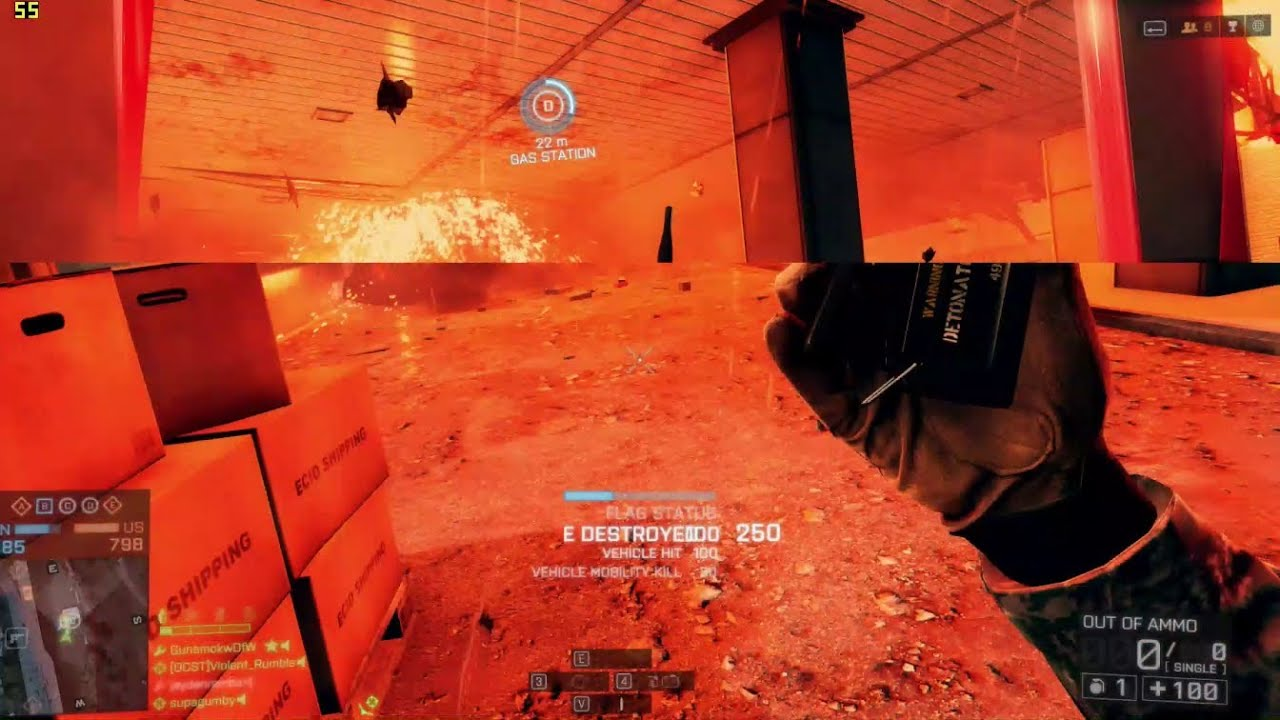
\includegraphics[width=\textwidth]{screen_tearing.jpg}
	\caption{Screen tearing} \cite{fig:screen_tearing}
\end{figure}

Here you can see that 2 images are displayed at the same time. The top image is the new one that has
not managed to fully render yet and the bottom image is the old one that was being displayed before the
refresh. Remember that we overwrite the old image with the new one when rendering. Because not every pixel
was done rendering when the refresh happened we get the rendered part and the old part displayed at the same time.
This is obviously not optimal and we want to avoid this. So let's move on to the next one.

The next present mode is called
\textit{VK\textunderscore PRESENT\textunderscore MODE\textunderscore FIFO\textunderscore KHR}.
FIFO stands for first in first out. This mode handles the images in a queue. Each fully rendered image
is added to the queue and the image that is at its front is displayed. The
\textit{VK\textunderscore PRESENT\textunderscore MODE\textunderscore FIFO\textunderscore KHR} mode
only swaps the framebuffers when the vertical blank happens and takes the framebuffer's image that is at the front
of the queue, which avoids the screen tearing effect. The problem with this mode is that if the queue is full,
aka each framebuffer's image is rendered but not displayed yet, the \ac{GPU} has to wait until the vertical blank happens
to continue rendering, which caps the frame rate to the refresh rate of the monitor. This is called v-sync and
causes a delay between the rendering and the displaying of the image, but is guaranteed
to be available and has a lower energy consumption than the other modes that have the \ac{GPU} rendering without a break.
Therefore this mode is the most common mode for mobile devices, but is still widely used for desktop applications.

There is a similar version of the
\textit{VK\textunderscore PRESENT\textunderscore MODE\textunderscore FIFO\textunderscore KHR} mode called \\
\textit{VK\textunderscore PRESENT\textunderscore MODE\textunderscore FIFO\textunderscore RELAXED\textunderscore KHR}.
This mode only differs from the previous mode in the way it handles a empty queue. If the queue is empty, aka no
framebuffer's image is rendered yet, the swapchain will swap the framebuffers immediately and display a teared image. This mode
is used when we have a long rendering time and want to avoid waiting for the queue to be filled.

Finally we have the \\
\textit{VK\textunderscore PRESENT\textunderscore MODE\textunderscore MAILBOX\textunderscore KHR} mode.
This is also the mode that we will be using. This mode is similar to the
\textit{VK\textunderscore PRESENT\textunderscore MODE\textunderscore FIFO\textunderscore KHR} mode,
with the difference that the swapchain will not let the \ac{GPU} idle when the queue is full. Instead it will
discard the image that is at the front of the queue and start rendering again. This constant rendering
will provide us with the lowest latency but also the highest energy consumption. But that should not
be a problem for our application.

We will simply iterate through the available present modes and return the \\
\textit{VK\textunderscore PRESENT\textunderscore MODE\textunderscore MAILBOX\textunderscore KHR} mode
if it is available. If not we will return the \textit{VK\textunderscore PRESENT\textunderscore MODE\textunderscore FIFO\textunderscore KHR} mode.

\begin{lstlisting}[Language=C++]
VkPresentModeKHR SwapChain::chooseSwapPresentMode(const std::vector<VkPresentModeKHR> &availablePresentModes) {
  for (const auto &availablePresentMode : availablePresentModes) {
      if (availablePresentMode == VK_PRESENT_MODE_MAILBOX_KHR)
        return availablePresentMode;
    }

  return VK_PRESENT_MODE_FIFO_KHR;
}
\end{lstlisting}

\subsection{Swapchain extent}

Like mentioned before we have to choose the extent of the swapchain images. We get the extent
from the devices capabilities. If the width and height of the extent are set to the maximum
value of uint32\_t, we are indicated that the extent is defined in screen coordinates and we
have to get the extent from our windowExtent variable. We then have to clamp
the extent to the minimum and maximum extent that the device supports tho. If the width and height
are not set to the maximum value we can use the extent directly because that tells us that the extent
is already in pixels.

\begin{lstlisting}[Language=C++]
VkExtent2D SwapChain::chooseSwapExtent(const VkSurfaceCapabilitiesKHR &capabilities) {
  if (capabilities.currentExtent.width != UINT32_MAX)
    return capabilities.currentExtent;
  else {
    VkExtent2D actualExtent = windowExtent;

    actualExtent.width = std::clamp(actualExtent.width, capabilities.minImageExtent.width, capabilities.maxImageExtent.width);
    actualExtent.height = std::clamp(actualExtent.height, capabilities.minImageExtent.height, capabilities.maxImageExtent.height);

    return actualExtent;
  }
}
\end{lstlisting}

\subsection{Image count}

The final thing we have to do is to set the min image count of the swapchain. The image count is the amount
of images that the swapchain will contain aka the amount of framebuffers. We will use one more than the
minimum image count that the device supports, for the min image count of the swapchain. This is because
we otherwise would have to wait for the driver to complete internal operations before we can acquire the
next image. Because we increase the min image count
by one we have to check if it is bigger than the max image count. If it is we set the min image count to the
max image count. Except if the max image count of the device is 0, which means that there is no maximum image count.

\begin{lstlisting}[Language=C++]
uint32_t imageCount = swapChainSupport.capabilities.minImageCount + 1;
if (swapChainSupport.capabilities.maxImageCount > 0 && imageCount > swapChainSupport.capabilities.maxImageCount)
  imageCount = swapChainSupport.capabilities.maxImageCount;
\end{lstlisting}

\subsection{Swapchain creation}

Now that we have all the data we need we can create the swapchain. We will populate the
\textit{VkSwapchainCreateInfo} struct with the data we have and additionally set the
image array layers to 1, which is the amount of layers that the image has. This is always
1 unless you are working with stereoscopic 3D applications. We also have to set the image
usage to
\textit{VK\textunderscore IMAGE\textunderscore USAGE\textunderscore COLOR\textunderscore ATTACHMENT\textunderscore BIT},
which means that we will render directly to the image.

\begin{lstlisting}[Language=C++]
VkSwapchainCreateInfo createInfo = {};
createInfo.sType = VK_STRUCTURE_TYPE_SWAPCHAIN_CREATE_INFO_KHR;
createInfo.surface = device.surface();
createInfo.minImageCount = imageCount;
createInfo.imageFormat = surfaceFormat.format;
createInfo.imageColorSpace = surfaceFormat.colorSpace;
createInfo.imageExtent = extent;
createInfo.imageArrayLayers = 1;
createInfo.imageUSage = VK_IMAGE_USAGE_COLOR_ATTACHMENT_BIT;
\end{lstlisting}

But that's not all. We also have to specify the sharing mode of the swapchain. The sharing mode
determines how the images are shared between multiple queue families. We use 2 queue families, the
graphics queue family and the present queue family. Now we have 2 cases. The first case is that the
graphics queue family and the present queue family have the same index. In this case we set the sharing
mode to exclusive. This means that an image is owned by one queue family at a time and has to be
explicitly transferred to the other queue family. In this case the count of queue families and the
queue family indices that are used are not relevant. The second case is that the graphics queue family
and the present queue family have different indices. In this case we set the sharing mode to concurrent.
This means that an image can be used by multiple queue families without explicit ownership transfers.
It is important to note that the queue family indices are relevant in this case, because the swapchain needs
to know what queue families can access the image.

We'll start off by getting the queue family indices from the device. We will then check if the graphics
queue family and the present queue family are different. If they are we set the sharing mode to concurrent
and set the queue family indices and their count. If they are the same we set the sharing mode to exclusive.

\begin{lstlisting}[Language=C++]
QueueFamilyIndices indices = device.findQueueFamilies();
if (indices.graphicsFamily.value() != indices.presentFamily.value()) {
   createInfo.imageSharingMode = VK_SHARING_MODE_CONCURRENT;
   createInfo.queueFamilyIndexCount = 2;
   uint32_t queueFamilyIndices[] = {indices.graphicsFamily.value(), indices.presentFamily.value()};
   createInfo.pQueueFamilyIndices = queueFamilyIndices;
} else {
   createInfo.imageSharingMode = VK_SHARING_MODE_EXCLUSIVE;
}
\end{lstlisting}

We're still not done yet! We also have to specify if and what kind of transformation we want
to apply to the images. For example we might want to flip or rotate the image. We don't want
anything to happen to the image so we set the pre transform to the current transform. We get
the current transform from the swapchain support details capabilities. We also have to specify
the composite alpha. The composite alpha is used to blend the window with other windows in the
system. We want to ignore the alpha channel so we set the composite alpha to the opaque bit.
Finally we specify our present mode, the clipped flag and the old swapchain. The clipped flag
indicates that we don't need the pixels that are obscured by other windows. If you need the
pixels to predict future frames you can set the clipped flag to false but we will keep it true.
The old swapchain is used to create a new swapchain from an old one. We will set it to
\textit{VK\textunderscore NULL\textunderscore HANDLE}, but will come back to this later.

\begin{lstlisting}[Language=C++]
createInfo.preTransform = swapChainSupport.capabilities.currenttransform;
createInfo.compositeAlpha = VK_COMPOSITE_ALPHA_OPAQUE_BIT_KHR;
createInfo.presentMode = presentMode;
createInfo.clipped = VK_TRUE;
createInfo.oldSwapchain = VK_NULL_HANDLE;
\end{lstlisting}

Now that we have the create info struct we can create the swapchain with the \textit{vkCreateSwapChainKHR}
function, that takes the device, the create info struct, a custom allocator and a pointer to the swapchain
variable that we also have to add to our header. We again will check for an error and throw an runtime
error if the creation was not successful.

\begin{lstlisting}[Language=C++]
if (vkCreateSwapChainKHR(device.device(), &createInfo. nullptr, &swapChain) != VK_SUCCESS)
  throw std::runtime_error("Failed to create swap chain!");
\end{lstlisting}

After the creation of the swapchain we need to store the images of the swapchain. We can get the images
with the \textit{vkGetSwapchainImagesKHR} function. We have to specify the device, the swapchain, a pointer
to the image count and a pointer to the images. We will store the images in the \textit{swapChainImages}
vector. Then we should also create a variable for the image format and the extent of the swapchain images
and store them in the class.

\begin{lstlisting}[Language=C++]
//swapchain.hpp
private:
  ...
  VkSwapchainKHR swapChain;
  VkFormat swapChainImageFormat;
  VkExtent2D swapChainExtent;
\end{lstlisting}

\begin{lstlisting}[Language=C++]
vkGetSwapchainImagesKHR(device.device(), swapChain, &imageCount, nullptr);
swapChainImages.resize(imageCount);
vkGetSwapchainImagesKHR(device.device(), swapChain, &imageCount, swapChainImages.data());

swapChainImageFormat = surfaceFormat.format;
swapChainExtent = extent;
\end{lstlisting}

If you ask yourself why we have to get the image count first and then resize the vector, it is because
we have only defined the minimum image count of the swapchain in the imageCount variable. The actual
image count could be different.

Now we have to make sure that the swapchain is destroyed in the destructor. We can do this by calling
the \textit{vkDestroySwapchainKHR} function.

\begin{lstlisting}[Language=C++]
SwapChain::~SwapChain() {
  vkDestroySwapchainKHR(device.device(), swapChain, nullptr);
}
\end{lstlisting}

\subsection{Image Views}

The swapchain in now created and we have the images stored in the \\
\textit{swapChainImages} vector. But like mentioned before,
we cannot read the images directly. It only stores data about the pixels and the main memory of the texture and misses
information like the format or the mipmapping level. To get the full image data we have to create an image view, that
stores the missing information. We will need a new function called \textit{createImageViews} that will be called after
the creation of the swapchain. We will also need a vector to store the image views, that we will size to the amount of
swapchain images in the function.

For each image in the \textit{swapChainImages} vector we will create an image view and define the image that we view
into, the desired format, the view type, the subresource range with the aspect mask, the base mip level, the level count,
the base array layer and the layer count. The view type defines how many dimensions the image has. We will use the 2D view
type because our pipeline returns a orthogonal 2D image. The aspect mask defines what the image view will be used for.
You might ask yourself why we have to define the aspect mask in the image view, when we already defined the image usage
in the swapchain creation. The reason for that is that we can use one image for multiple purposes. For example we can use
one image for color and depth attachments. The view might only need the color information, so we have to define the aspect
mask in the image view to reduce the amount of data that is stored in the view. We will use the color aspect mask for now.
We will also keep the same format as the swapchain image format, but for some use cases you might want to use a different
format that is compatible with the surface format.

Before we go further I'd like to explain what mipmapping is and what a mip level is. Mipmapping is a technique that
is similar to \ac{LOD}, but is used for textures. It reduces the textures resolution when the texture
is far away from the camera. This fixes an interesting problem that occurs when rendering textures. Would we keep the same
resolution for the texture when the texture is far away from the camera, the texture create a so called moiré pattern.
It occures because we try to map a high resolution texture on a area that is to small.

\begin{figure}[htbp]
	\centering
	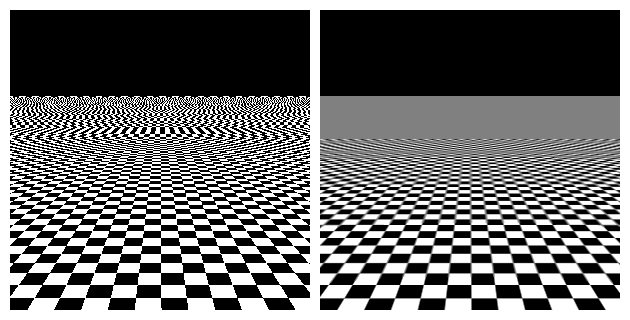
\includegraphics[width=\textwidth]{mipmapping.png}
	\caption{Mipmapping(left: moiré pattern, right: mipmapping)} \cite{fig:mipmapping}
\end{figure}

By reducing the resolution of the texture we can avoid this problem.
When we reduce the resolution of the texture we create a new texture that is half the size of the original texture.
So when we have a texture with a resolution of 256x256 we create a new texture with a resolution of 128x128 and so on,
until we reach a resolution of 1x1. The different textures are called mip levels.

Now that we now that we can set the base mip level that basically sets the first mip level that is used. We will set it to 0
we get the original resolution of the texture. The level count defines how many mip levels we want to use. We will set it to 1
for now. The base array layer defines the first layer that is used. We will set it to 0 because we will only use one layer.
The layer count defines how many layers we want to use. We will keep it at 1 for now.

\begin{lstlisting}[Language=C++]
SwapChain::SwapChain(Device &device, VkExtent2D extent) : device{device}, windowExtent{extent} {
  createSwapChain();
  createImageViews();
}

void SwapChain::createImageViews() {
  swapChainImageViews.resize(swapChainImages.size());

  for (size_t i = 0; i < swapChainImages.size(); i++) {
    VkImageViewcreateInfo.viewInfo = {};
    viewInfo.sType = VK_STRUCTURE_TYPE_IMAGE_VIEW_CREATE_INFO;
    viewInfo.image = swapChainImages[i];
    viewInfo.format = swapChainImageFormat;
    viewInfo.viewType = VK_IMAGE_VIEW_TYPE_2D;
    viewInfo.subresourceRange.aspectMask = VK_IMAGE_ASPECT_COLOR_BIT;
    viewInfo.subresourceRange.baseMipLevel = 0;
    viewInfo.subresourceRange.levelCount = 1;
    viewInfo.subresourceRange.baseArrayLayer = 0;
    viewInfo.subresourceRange.layerCount = 1;

    if (vkCreateImageview(device.device(), &viewInfo, nullptr, &swapChainImageViews[i]) != VK_SUCCESS)
      throw std::runtime_error("Failed to create image views!");
  }
}
\end{lstlisting}

Great! Let's try to run the application. To do so we have to add the swapchain to the application class.
Because the swapchain takes the device and the extent as arguments we have to add a getter function to the
surface class that returns the extent. We will also add a getter to the device class that returns the
logical device.

\begin{lstlisting}[Language=C++]
//device.hpp
public:
  ...
  VkDevice device() { return device_; }
\end{lstlisting}

\begin{lstlisting}[Language=C++]
//surface.hpp
public:
  ...
  VkExtent2D getExtent() { return{static_cast<uint32_t>(width), static_cast<uint32_t>(height)}; }
\end{lstlisting}

\begin{lstlisting}[Language=C++]
//app.hpp
private:
  ...
  SwapChain swapChain{device, window.getExtent()};
\end{lstlisting}

If everything is set up correctly so far the code should run.

Okay when closing the application we get an error that tells us to destroy the image views before the device.
This is important because we have to destroy all child objects before we destroy the parent object.

So let's destroy the image views in the destructor of the swapchain class. We can do this by calling the
\textit{vkDestroyImageView} function for each image view in the \textit{swapChainImageViews} vector.

\begin{lstlisting}[Language=C++]
SwapChain::~SwapChain() {
  for (const VkImageView &imageView : swapChainImageViews)
    vkDestroyImageView(device.device(), imageView, nullptr);

  vkDestroySwapchainKHR(device.device(), swapChain, nullptr);
}
\end{lstlisting}

We don't have to destroy the swapchain images because they are destroyed with the swapchain.

\subsection{Render Pass}

Before we can render anything we need to create a render pass. A render pass contains information about
the amount of color and depth buffers, how many samples are used for them and how the data is handled
during rendering.

Let's add a new function called \textit{createRenderPass} to the swapchain class.

\begin{lstlisting}[Language=C++]
SwapChain::SwapChain(Device &device, VkExtent2D extent) : device{device}, windowExtent{extent} {
  createSwapChain();
  createImageViews();
  createRenderPass();
}

void SwapChain::createRenderPass() {}
\end{lstlisting}

Inside we will need to create 2 attachments. One for the color buffer and one for the depth buffer.
Let's start with the color attachment. We will have to populate the \textit{VkAttachmentDescription} struct
with the format, the sample count, the load and store operation, the stencil load and store operation, the initial
and the final layout. For the color attachment we will use the swapchain image format. The sample count defines how
\ac{MSAA} is handled. Let's rewind shortly how \ac{MSAA} works.

When we render a polygon we rasterize it into fragments. Each fragment is a pixel that is covered by the polygon.
The graphics pipeline determines which pixel to color by checking if the polygon covers the center of the pixel.
But this returns a jagged edge. To fix this we can use \acro{MSAA}. \acro{MSAA} works by sampling multiple points in the pixel
and then averaging the color of the points. This creates a smoother edge. We can define how many samples we want to use
in each fragment.

Okay back to the color attachment. We will use 1 sample for now. The load operation defines what to do with the data
in the attachment before rendering. We will clear the frame buffer before rendering, because we don't need it.
That means we have to set it to \textit{VK\textunderscore ATTACHMENT\textunderscore LOAD\textunderscore OP\textunderscore CLEAR}.
When you need it to be preserved you can set it to
\textit{VK\textunderscore ATTACHMENT\textunderscore LOAD\textunderscore OP\textunderscore LOAD}. The store
operation defines what to do with the data in the attachment after rendering. We will store the data in the frame buffer
after rendering, with the \textit{VK\textunderscore ATTACHMENT\textunderscore STORE\textunderscore OP\textunderscore STORE}
value. It is also possible to say that you don't care about the data in the attachment before or after rendering
by setting the store or load operation to
\textit{VK\textunderscore ATTACHMENT\textunderscore STORE/LOAD \textunderscore OP\textunderscore DONT\textunderscore CARE}.

The stencil load and store operation are used for the stencil buffer. Wait what is a stencil buffer? A stencil buffer
is another buffer that allows us to further manipulate pixels combined with the depth buffer. For example we can
create outlines around objects by creating another object with a slightly bigger size and add a stencil buffer to it with a
reference value. When rendering the outline we can perform a stencil test that checks if the pixels reference value is
equal to 1 and only render the pixels that don't pass the test. The stencil load and store operation work the same way
as the load and store operation we don't really care about the stencil buffer for now so we will set the operations to
\textit{VK\textunderscore ATTACHMENT\textunderscore LOAD/STORE\textunderscore OP\textunderscore DONT\textunderscore CARE}.
Finally the initial and final layout define how the image is handled before and after the render pass. The initial layout
is set to \textit{VK\textunderscore IMAGE\textunderscore LAYOUT\textunderscore UNDEFINED} because we don't care about the
image before the render pass. The final layout is set to
\textit{VK\textunderscore IMAGE\textunderscore LAYOUT\textunderscore PRESENT\textunderscore SRC\textunderscore KHR},
which means that the image will be presented to the swapchain.

\begin{lstlisting}[Language=C++]
void SwapChain::createRenderPass() {
  VkAttachmentDescription colorAttachment = {};
  colorAttachment.format = swapChainImageFormat;
  colorAttachment.samples = VK_SAMPLE_COUNT_1_BIT;
  colorAttachment.loadOp = VK_ATTACHMENT_LOAD_OP_CLEAR;
  colorAttachment.storeOp = VK_ATTACHMENT_STORE_OP_STORE;
  colorAttachment.stencilLoadOp = VK_ATTACHMENT_LOAD_OP_DONT_CARE;
  colorAttachment.stencilStoreOp = VK_ATTACHMENT_STORE_OP_DONT_CARE;
  colorAttachment.initialLayout = VK_IMAGE_LAYOUT_UNDEFINED;
  colorAttachment.finalLayout = VK_IMAGE_LAYOUT_PRESENT_SRC_KHR;
}
\end{lstlisting}

After that we need to create a \textit{VkAttachmentReference} that stores the index and layout type.
The color attachment will be our first attachment and has the \\
\textit{VK\textunderscore IMAGE\textunderscore LAYOUT\textunderscore COLOR\textunderscore ATTACHMENT\textunderscore OPTIMAL}.

\begin{lstlisting}[Language=C++]
VkAttachmentReference colorAttachmentRef = {};
colorAttachmentRef.attachment = 0;
colorAttachmentRef.layout = VK_IMAGE_LAYOUT_COLOR_ATTACHMENT_OPTIMAL;
\end{lstlisting}

Now we do the same for the depth attachment. For the format we will need a helper function that finds us a suitable
depth format called \textit{findDepthFormat}. This function calls the \textit{findSupportedFormat} function that we
will need to implement in the device class. The \textit{findSupportedFormat} function takes a vector of formats,
how the image is stored aka the tiling and the features.

Inside the \textit{findSupportedFormat} function we will iterate through the formats, get their properties with the
\textit{vkGetPhysicalDeviceFormatProperties} function and check if the properties tiling features are equal to the
features that we passed to the function. If it is we will return the format. We will check for 2 tilings,
the linear and the optimal tiling. The linear tiling mode stores the image in a linear order, which means that the
image is stored in a row like a 2D array. The optimal tiling mode stores the image in an oder that is optimized for
\ac{GPU} access. We will use the optimal tiling mode for the depth format. We will check the following formats:
\textit{VK\textunderscore FORMAT\textunderscore D32\textunderscore SFLOAT},
\textit{VK\textunderscore FORMAT\textunderscore D32\textunderscore SFLOAT\textunderscore S8\textunderscore UINT} and
\textit{VK\textunderscore FORMAT\textunderscore D24\textunderscore UNORM\textunderscore S8\textunderscore UINT}.

The first format is a 32 bit float format that is used for depth buffers. The second format is a two channel format
with a 32 bit float for the depth and a 8 bit unsigned integer for the stencil buffer. The third format is a 24 bit
float format for the depth and a 8 bit unsigned integer for the stencil buffer. We will parse in all 3 of them but if you need
a stencil buffer you should use the second or third format. For the features we will use the
\textit{VK\textunderscore FORMAT\textunderscore FEATURE\textunderscore DEPTH\textunderscore STENCIL\textunderscore ATTACHMENT\textunderscore BIT}

\begin{lstlisting}[Language=C++]
//swapchain.cpp
void SwapChain::createRenderPass(){
  ...
  VkAttachmentDescription depthAttachment = {};
  depthAttachment.format = findDepthFormat();
  depthAttachment.samples = VK_SAMPLE_COUNT_1_BIT;
  depthAttachment.loadOp = VK_ATTACHMENT_LOAD_OP_CLEAR;
  depthAttachment.storeOp = VK_ATTACHMENT_STORE_OP_DONT_CARE;
  depthAttachment.stencilLoadOp = VK_ATTACHMENT_LOAD_OP_DONT_CARE;
  depthAttachment.stencilStoreOp = VK_ATTACHMENT_STORE_OP_DONT_CARE;
  depthAttachment.initialLayout = VK_IMAGE_LAYOUT_UNDEFINED;
  depthAttachment.finalLayout = VK_IMAGE_LAYOUT_DEPTH_STENCIL_ATTACHMENT_OPTIMAL;

  VkAttachmentReference depthAttachmentRef = {};
  depthAttachmentRef.attachment = 1;
  depthAttachmentRef.layout = VK_IMAGE_LAYOUT_DEPTH_STENCIL_ATTACHMENT_OPTIMAL;
}

VkFormat SwapChain::findDepthFormat() {
  return device.findSupportedFormat(
    {VK_FORMAT_D32_SFLOAT, VK_FORMAT_D32_SFLOAT_S8_UINT, VK_FORMAT_D24_UNORM_S8_UINT},
    VK_IMAGE_TILING_OPTIMAL,
    VK_FORMAT_FEATURE_DEPTH_STENCIL_ATTACHMENT_BIT
  );
}
\end{lstlisting}

\begin{lstlisting}[Language=C++]
//device.cpp
VkFormat Device::findSupportedFormat(const std::vector<VkFormat> &candidates, VkImageTiling tiling, VkFormatFeatureFlags features) {
  for (VkFormat format : candidates) {
    VkFormatproperties props;
    vkGetPhysicalDeviceFormatProperties(physicalDevice, format, &props);

    if (tiling == VK_IMAGE_TILING_LINEAR && (props.linearTilingFeatures & features) == features)
      return format;
    else if (tiling == VK_IMAGE_TILING_OPTIMAL && (props.optimalTilingFeatures & features) == features)
      return format;
  }

  throw std::runtime_error("Failed to find supported format!");
}
\end{lstlisting}

We don't care about the depth data after rendering so we set the store operation to
\textit{VK\textunderscore ATTACHMENT\textunderscore STORE\textunderscore OP\textunderscore DONT\textunderscore CARE}.

A renderpass can consist of multiple subpasses. A subpass is a rendering operation that takes the output of the previous
subpass as input. We will only use one subpass for now, but using multiple subpasses can be useful for post processing
effects. We will create a \textit{VkSubpassDescription} struct that contains the pipeline bind point, the amount of color
attachments, a pointer to the color attachments and a pointer to the depth stencil attachment. There is more data that
we can add to the subpass description, but don't need for now. The pipeline bind point defines if the subpass is used
for graphics or compute operations. We will use the graphics pipeline bind point.

\begin{lstlisting}[Language=C++]
void SwapChain::createRenderPass() {
  ...
  VkSubpassDescription subpass = {};
  subpass.pipelineBindPoint = VK_PIPELINE_BIND_POINT_GRAPHICS;
  subpass.colorAttachmentCount = 1;
  subpass.pColorAttachments = &colorAttachmentRef;
  subpass.pDepthStencilAttachment = &depthAttachmentRef;
}
\end{lstlisting}

There is one problem with the subpass description. When we have multiple subpasses we might get a case where one subpass
writes to an attachment and the next subpass reads from it, while the first subpass is not finished. This turns out
to be a race condition and is falsifying the results. To avoid this we can use subpass dependencies. A subpass dependency
tells the render pass when to start and end the subpass. We will create a \textit{VkSubpassDependency} struct that contains
the indices of the previous and the next subpass, the stage mask and the access mask. The \textit{srcSubpass} defines
where the dependency starts and the \textit{dstSubpass} defines where the dependency ends. In our case our dependency
starts outside of the subpass, which means that we have to set the \textit{srcSubpass} to
\textit{VK\textunderscore SUBPASS\textunderscore EXTERNAL}. Because we only have one subpass we can set the
\textit{dstSubpass} to 0. The stage mask defines what stages of the pipeline the dependency is waiting for. We will
wait for the color attachment output stage, which refers to any operations that render to the color attachment, and
the early fragment test stage, which refers to the depth and stencil tests. The access mask defines what kind of
operations the dependency will wait for. The source will not wait for any operations, so we set it to 0. The destination
will wait until the color attachment is written to and the depth and stencil buffer is written to. We will set it to
\textit{VK\textunderscore ACCESS\textunderscore COLOR\textunderscore ATTACHMENT\textunderscore WRITE\textunderscore BIT}
and \textit{VK\textunderscore ACCESS\textunderscore DEPTH\textunderscore STENCIL\textunderscore ATTACHMENT\textunderscore WRITE\textunderscore BIT}.

\begin{lstlisting}[Language=C++]
void SwapChain::createRenderPass() {
  ...
  VkSubpassDependency dependency = {};
  dependency.srcSubpass = VK_SUBPASS_EXTERNAL;
  dependency.dstSubpass = 0;
  dependency.srcStageMask = VK_PIPELINE_STAGE_COLOR_ATTACHMENT_OUTPUT_BIT | VK_PIPELINE_STAGE_EARLY_FRAGMENT_TESTS_BIT;
  dependency.dstAccessMask = 0;
  dependency.dstStageMask = VK_PIPELINE_STAGE_COLOR_ATTACHMENT_OUTPUT_BIT | VK_PIPELINE_STAGE_EARLY_FRAGMENT_TESTS_BIT;
  dependency.dstAccessMask = VK_ACCESS_COLOR_ATTACHMENT_WRITE_BIT | VK_ACCESS_DEPTH_STENCIL_ATTACHMENT_WRITE_BIT;
}
\end{lstlisting}

Now that we know how the attachments and subpasses are connected we can create the render pass. We will create a
\textit{VkRenderPass} variable in the header of the swapchain class. Then we will
populate the \textit{VkRenderPassCreateInfo} struct with the color and depth attachment, the subpass, the dependency
and the attachment count. Let's first go ahead and create an array of attachments that contains the color and depth
attachment. Then we add the sType and the other data to the render pass create info, create the render pass and
throw an error if the creation was not successful.

\begin{lstlisting}[Language=C++]
//swapchain.hpp
private:
  ...
  VkRenderPass renderPass;
\end{lstlisting}

\begin{lstlisting}[Language=C++]
void SwapChain::createRenderPass() {
  ...
  std::array<VkAttachmentDescription, 2> attachments = {colorAttachment, depthAttachment};

  VkRenderPasscreateInfo.renderPassInfo = {};
  renderPassInfo.sType = VK_STRUCTURE_TYPE_RENDER_PASS_CREATE_INFO;
  renderPassInfo.attachmentCount = static_cast<uint32_t>(attachments.size());
  renderPassInfo.pattachments = attachments.data();
  renderPassInfo.subpassCount = 1;
  renderPassInfo.pSubpasses = &subpass;
  renderPassInfo.dependencyCount = 1;
  renderPassInfo.pDependencies = &dependency;

  if (vkCreateRenderPass(device.device(), &renderPassInfo, nullptr, &renderPass) != VK_SUCCESS)
    throw std::runtime_error("failed to create render pass!");
}
\end{lstlisting}

Finally we have to make sure to destroy the render pass.

\begin{lstlisting}[Language=C++]
SwapChain::~SwapChain() {
  ...
  vkDestroyRenderPass(device.device(), renderPass, nullptr);
}
\end{lstlisting}

\subsection{Depth Resources}

Just like the color image we have to create an depth image and an depth image view. We will create a new function
called \textit{createDepthResources} that will be called after the creation of the render pass. We will also need
a new variable in the header of the swapchain class that stores the depth images and the depth image views. We will need one
depth image and one depth image view for each swapchain image. The problem is that when we create the depth image on the \ac{CPU} we
need to allocate memory on the \ac{GPU} and then bind the image to that memory, because we need the data there.
For that we will need a new function in the device class called \textit{createImageWithInfo}.
This function will take an image info struct, a memory property flag, a pointer to the image and a pointer to the image memory.

\begin{lstlisting}[Language=C++]
//swapchain.hpp
private:
  ...
  void createDepthResources();

  std::vector<VkImage> depthImages;
  std::vector<VkDeviceMemory> depthImageMemories;
  std::vector<VkImageView> depthImageViews;
\end{lstlisting}

\begin{lstlisting}[Language=C++]
SwapChain::SwapChain(Device &device, VkExtent2D extent) : device{device}, windowExtent{extent} {
  createSwapChain();
  createImageViews();
  createRenderPass();
  createDepthResources();
}

void SwapChain::createDepthResources() {
  depthImages.resize(swapChainImages.size());
  depthImageMemories.resize(swapChainImages.size());
  depthImageViews.resize(swapChainImages.size());

  VkFormat depthFormat = findDepthFormat();
  swapChainDepthFormat = depthFormat;

  for (size_t i = 0; i < swapChainImages.size(); i++) {
    VkImageCreateInfo.imageInfo = {};
    imageInfo.sType = VK_STRUCTURE_TYPE_IMAGE_CREATE_INFO;
    imageInfo.imageType = VK_IMAGE_TYPE_2D;
    imageInfo.extent.width = swapChainExtent.width;
    imageInfo.extent.height = swapChainExtent.height;
    imageInfo.extent.depth = 1;
    imageInfo.mipLevels = 1;
    imageInfo.arraylayers = 1;
    imageInfo.format = depthFormat;
    imageInfo.tiling = VK_IMAGE_TILING_OPTIMAL;
    imageInfo.initialLayout = VK_IMAGE_LAYOUT_UNDEFINED;
    imageInfo.usage = VK_IMAGE_USAGE_DEPTH_STENCIL_ATTACHMENT_BIT;
    imageInfo.samples = VK_SAMPLE_COUNT_1_BIT;
    imageInfo.sharingMode = VK_SHARING_MODE_EXCLUSIVE;
    imageInfo.flags = 0;

    device.createImageWithInfo(imageInfo, VK_MEMORY_PROPERTY_DEVICE_LOCAL_BIT, depthImages[i], depthImageMemories[i]);

    VkImageViewcreateInfo.viewInfo = {};
    viewInfo.sType = VK_STRUCTURE_TYPE_IMAGE_VIEW_CREATE_INFO;
    viewInfo.image = depthImages[i];
    viewInfo.viewType = VK_IMAGE_VIEW_TYPE_2D;
    viewInfo.format = depthFormat;
    viewInfo.subresourceRange.aspectMask =  VK_IMAGE_ASPECT_DEPTH_BIT;
    viewInfo.subresourceRange.baseMipLevel = 0;
    viewInfo.subresourceRange.levelCount = 1;
    viewInfo.subresourceRange.baseArrayLayer = 0;
    viewInfo.subresourceRange.layerCount = 1;

    if (vkCreateImageView(device.device(), &viewInfo, nullptr, &depthImageViews[i]) != VK_SUCCESS)
      throw std::runtime_error("Failed to create image views!");
 }
}
\end{lstlisting}

The \textit{createImageWithInfo} function first creates the image with the \textit{vkCreateImage} function. Then it
gets the memory requirements of the image with the \textit{vkGetImageMemoryRequirements} function. We will then
populate the \textit{VkMemoryAllocateInfo} struct with the sType, allocation size and the memory type index. We will
get the memory type index with the \textit{findMemoryType} function that we will implement next. After that we
allocate the memory with the \textit{vkAllocateMemory} function and bind the memory to the image with the
\textit{vkBindImageMemory} function.

\begin{lstlisting}[Language=C++]
//device.cpp
void Device::createImageWithInfo(const VkImageCreateInfo.&imageInfo, 
                                 vkMemeroryPropertyflags properties, 
                                 VkImage &image, 
                                 VkDeviceMemory &imageMemory) {
  if (vkCreateImage(device_, &imageInfo, nullptr, &image) != VK_SUCCESS)
    throw std::runtime_error("Failed to create image!");

  VkMemoryRequirements memRequirements;
  vkGetImageMemoryRequirements(device_, image, &memRequirements);

  VkMemoryAllocateInfo allocInfo = {};
  allocInfo.sType = VK_STRUCTURE_TYPE_MEMORY_ALLOCATE_INFO;
  allocInfo.allocationsize = memRequirements.size;
  allocInfo.memoryTypeIndex = findMemoryType(memRequirements.memoryTypeBits, properties);

  if (vkAllocateMemory(device_, &allocInfo, nullptr, &imageMemory) != VK_SUCCESS)
    throw std::runtime_error("Failed to allocate image memory!");

  if (vkBindImageMemory(device_, image, imageMemory, 0) != VK_SUCCESS)
    throw std::runtime_error("Failed to bind image memory!");
}
\end{lstlisting}

The \textit{findMemoryType} function will iterate through the memory types of the physical device and check if the
properties are supported. If it is it will return the memory type index.

\begin{lstlisting}[Language=C++]
//device.cpp
uint32_t Device::findMemoryType(uint32_t typeFilter, vkMemeroryPropertyflags properties) {
  VkPhysicalDeviceMemeroryProperties memProperties;
  vkGetPhysicalDeviceMemeroryProperties(physicalDevice, &memProperties);

  for (uint32_t i = 0; i < memProperties.memoryTypeCount; i++) {
    if ((typeFilter & (1 << i)) && (memProperties.memoryTypes[i].propertyFlags & properties) == properties)
      return i;
  }

  throw std::runtime_error("Failed to find suitable memory type!");
}
\end{lstlisting}

In the if statement we first filter the types by going through the bits of the type filter. Then we check if the
properties are supported by the memory type. If it is we return the memory type index.

Now that we have the depth resources we have to destroy them and clear the \ac{GPU} memory in the destructor of the swapchain class.

\begin{lstlisting}[Language=C++]
SwapChain::~SwapChain() {
  ...
  for (size_t i = 0; i < depthImages.size(); i++) {
      vkDestroyImageView(device.device(), depthImageViews[i], nullptr);
      vkDestroyImage(device.device(), depthImages[i], nullptr);
      vkFreeMemory(device.device(), depthImageMemories[i], nullptr);
    }
}
\end{lstlisting}

\subsection{Framebuffers}

Now that we have all our resources we can create the framebuffers. A framebuffer consists of the attachments and depth
resources that are used in the render pass. We will create a new function called \textit{createFramebuffers}
that will be called after the creation of the depth resources. We will also need a
new variable in the header of the swapchain class that stores the framebuffers.

\begin{lstlisting}[Language=C++]
//swapchain.hpp
private:
  ...
  void createFramebuffers();

  std::vector<VkFramebuffer> framebuffers;
\end{lstlisting}

To create the framebuffers we will iterate through the image views and create a framebuffer for each image view.
The create information for the framebuffer takes the render pass, the amount of attachments, the attachments, the width
and the height of the framebuffer and the layers count the framebuffer is used for. We will set the layers count to 1
and the width and height to the width and height of the swapchain extent.

\begin{lstlisting}[Language=C++]
SwapChain::SwapChain(Device &device, VkExtent2D extent) : device{device}, windowExtent{extent} {
  createSwapChain();
  createImageViews();
  createRenderPass();
  createDepthResources();
  createFramebuffers();
}

void SwapChain::createFramebuffers() {
  framebuffers.resize(swapChainImages.size());

  for (size_t i = 0; i < swapChainImages.size(); i++) {
    std::array<VkImageView, 2> attachments = {
      swapChainImageViews[i],
      depthImageViews[i]
    };

    VkFramebufferCreateInfo framebufferInfo = {};
    framebufferInfo.sType = VK_STRUCTURE_TYPE_FRAMEBUFFER_CREATE_INFO;
    framebufferInfo.renderpass = renderpass;
    framebufferInfo.attachmentCount = static_cast<uint32_t>(attachments.size());
    framebufferInfo.pAttachments = attachments.data();
    framebufferInfo.width = swapChainExtent.width;
    framebufferInfo.height = swapChainExtent.height;
    framebufferInfo.layers = 1;

    if (vkCreateFramebuffer(device.device(), &framebufferInfo, nullptr, &framebuffers[i]) != VK_SUCCESS)
      throw std::runtime_error("Failed to create framebuffer!");
  }
}
\end{lstlisting}

After that we have to destroy the framebuffers in the destructor of the swapchain class.

\begin{lstlisting}[Language=C++]
SwapChain::~SwapChain() {
  ...
  for (auto framebuffer : framebuffers) {
    vkDestroyFramebuffer(device.device(), framebuffer, nullptr);
  }
}
\end{lstlisting}

That's it! We now have all the objects that we need to render something. Let's shortly go through the steps that we have
done so far.

We began by creating the swapchain, which created the images and defined how the images are presented to the surface.
Then we defined how the images are viewed with the image views. After that we created a render pass, that stores the
color and depth attachments and ensures that the subpasses are not out of sync. We then created the depth resources that
include the depth image and the depth image view. Finally we created the framebuffers that store the attachments and depth
resources that are used in the render pass.

\section{Pipeline}

We can now start with the pipeline creation. Let's go ahead and create a new class called \textit{pipeline} that will
contain the pipeline creation. We will need a new function called \textit{createGraphicsPipeline} that will be called
in the constructor. This function takes the Path to the vertex and fragment shader and a PipelineConfigInfo struct that
we will define in the header of the pipeline class. We will also need a variable that stores the graphics pipeline, the
device and the shader modules.

\begin{lstlisting}[Language=C++]
//pipeline.hpp
struct PipelineConfigInfo {
  PipelineConfigInfo() = default;
  PipelineConfigInfo(const PipelineConfigInfo &) = delete;
  PipelineConfigInfo &operator=(const PipelineConfigInfo &) = delete;

  VkPipelineViewportStateCreateInfo viewportinfo;
  VkPipelineInputAssemblyStateCreateInfo inputAssemblyInfo;
  VkPipelineRasterizationStateCreateInfo rasterizationInfo;
  VkPipelineMultisampleStateCreateInfo mutlisampleInfo;
  VkPipelineColorBlendAttachmentState colorBlendAttachment;
  VkPipelineColorBlendStateCreateInfo colorBlendInfo;
  VkPipelineDepthStencilStateCreateInfo depthStencilInfo;
  std::vector<VkDynamicState> dynamicStates;
  VkPipelineDynamicStateCreateInfo dynamicStateinfo;
  VkPipelineLayout pipelineLayout = nullptr;
  VkRenderPass renderPass = nullptr;
  uint32_t subpass = 0;
};

class pipeline {
public:
  Pipeline(Device &device, const std::string &vertPath, const std::string &fragPath, const pipelineconfig &configInfo);
  ~Pipeline();

  Pipeline(const pipeline &) = delete;
  pipeline operator=(const pipeline &) = delete;

private:
  Device &device;
  VkPipeline graphicspipeline;
  VkShaderModule vertShaderModule;
  VkShaderModule fragShaderModule;
};
\end{lstlisting}

The PipelineConfigInfo struct contains all the information that we need to create the pipeline, like the create informations
for the states, the render pass, the subpass and the pipeline layout.

The constructor of the pipeline class will call the \textit{createGraphicsPipeline} function and set our device variable.

In the \textit{createGraphicsPipeline} function we will first check if the config info has a valid pipeline layout and render pass.
Then we will have to read the shader files and create the shader modules. Let's start off by adding a helper function called
\textit{readFile} that reads the shader files and returns the content as a vector of chars.

\begin{lstlisting}[Language=C++]
//pipeline.cpp
std::vector<char> Pipeline::readFile(const std::string &path) {
  std::ifstream file{Path, std::ios::ate | std::ios::binary};

  if (!file.is_open())
    throw std::runtime_error("Failed to open file: " + path);

  size_t filesize = static_cast<size_t>(file.tellg());
  std::vector<char> buffer(filesize);

  file.seekg(0);
  file.read(buffer.data(), filesize);

  file.close();
  return buffer;
}
\end{lstlisting}

This function opens a file. The \textit{std::ios::ate} flag sets the position of the file pointer to the end of the file and the
\textit{std::ios::binary} flag reads the file as binary. We have binary files because we have to compile our shaders to spir-v.
We go to the end of the file at the beginning because we want to create a buffer with the size of the file. Then we read the
file into the buffer and return the buffer.

We will do this for both the vertex and the fragment shader. We will then create the shader modules with another helper function.
The \textit{createShaderModule} function takes a vector of chars and a pointer to the shader module variable.

\begin{lstlisting}[Language=C++]
//pipeline.cpp
Pipeline::Pipeline(Device &device, const std::string &vertPath, const std::string &fragPath, const PipelineConfigInfo &configInfo)
: device{device} {
		createGraphicsPipeline(vertPath, fragPath, configInfo);
	}

void Pipeline::createGraphicsPipeline(const std::string &vertPath, const std::string &fragPath, const PipelineConfigInfo &configInfo) {
  assert(configInfo.pipelineLayout != VK_NULL_HANDLE && "Cannot create graphics pipeline. Invalid pipeline layout!");
  assert(configInfo.renderPass != VK_NULL_HANDLE && "Cannot create graphics pipeline. Invalid render pass!");

  std::vector<char> vertCode = readFile(vertPath);
  std::vector<char> fragCode = readFile(fragPath);

  createShaderModule(vertCode, &vertShaderModule);
  createShaderModule(fragCode, &fragShaderModule);
}

void Pipeline::createShaderModule(const std::vector<char> &code, VkShaderModule *shaderModule) {
  VkShaderModuleCreateInfo createInfo = {};
  createInfo.sType = VK_STRUCTURE_TYPE_SHADER_MODULE_CREATE_INFO;
  createInfo.codeSize = code.size();
  createInfo.pCode = reinterpret_cast<const uint32_t *>(code.data());

  if (vkCreateShaderModule(device.device(), &createInfo. nullptr, shaderModule) != VK_SUCCESS)
    throw std::runtime_error("Failed to create shader module!");
}
\end{lstlisting}

The \textit{createShaderModule} function creates a shader module with the \textit{vkCreateShaderModule} function. The
\textit{VkShaderModuleCreateInfo} struct contains the size of the code and the code itself. We have to cast the code to
a \textit{const uint32\textunderscore t} pointer because the code is a vector of chars but is actually binary data.
This binary data is what the \textit{vkCreateShaderModule} function expects.

\subsection{Shader Stages}

Okay before we go further into the pipeline creation we have to actually write and compile the shaders. We will use the
\ac{GLSL} for the shaders. Let's create a new folder in our src folder called shaders. In this folder we will create
a \textit{shader.vert} and a \textit{shader.frag} file.

We will start off with a simple vertex shaders that basically just pass the vertex position and the color to the fragment shader.
\ac{GLSL} looks very similar to C++ but has some differences. For example we have to define the version of the glsl language
at the beginning of the shader. We will use version 460. Next we create some vertex positions, from which we will create a simple triangle.
We will then have a void main function that sets the \textit{gl\textunderscore Position} variable to the vertex position.

For the fragment shader we will also define the version at the beginning. We will then have a layout out qualifier that outputs the
color to the next stage. We will then have a void main function that will set the out color to red.

\begin{lstlisting}[Language=C++]
//shader.vert
#version 460

vec3 positions[3] = vec3[](
  vec2(0.0, 0.5, 0.0),
  vec2(-0.5, -0.5, 0.0),
  vec2(0.5, -0.5, 0.0)
);

void main() {
  gl_Position = vec4(positions[gl_VertexIndex], 1.0);
}
\end{lstlisting}

You can see that we have this mysterious \textit{gl\textunderscore Position} variable. This is a built-in variable that
takes the vertex position as a 4d vector. The 4th component is the w component that is used for perspective division.
This \textit{gl\textunderscore Position} variable is a predefined out variable that is used to pass the vertex position
to the next stage. The \textit{gl\textunderscore VertexIndex} is also a built-in variable that is used to get the index
of the vertex that is currently processed.

\begin{lstlisting}[Language=C++]
//shader.frag
#version 460
layout(location = 0) out vec4 outColor;

void main() {
  outColor = vec4(1.0, 0.0, 0.0, 1.0);
}
\end{lstlisting}

Here we set the \textit{outColor} to the color that we passed from the vertex shader. The \textit{outColor} is a 4d vector
that represents the color of the pixel. The 4th component is the alpha value of the color.

Now that we have them we have to compile them to spir-v. We will simply add a compile.sh script that compiles the shaders. We will
use the \ac{GLSL} compiler that comes with the Vulkan SDK. The \ac{GLSL} compiler takes the shader file and then compiles
them to a specified output file. We will compile the vertex shader to \textit{shader.vert.spv} and the fragment shader to
\textit{shader.frag.spv}.

\begin{lstlisting}[Language=bash]
/usr/local/bin/glslc src/shaders/shader.vert -o src/shaders/shader.vert.spv
/usr/local/bin/glslc src/shaders/shader.frag -o src/shaders/shader.frag.spv
\end{lstlisting}

We will execute this script in our makefile before we compile the Vulkan application.
Simply add the following line to the makefile, before the compile line.

\textit{sh src/shaders/compile.sh}

Perfect! Now we have the shaders that the pipeline will read and use. Later you might add more shaders for more complex
rendering, but the vertex and fragment shader are mandatory.

We now have to create the actual stages and will begin with the shader stages. If you're wondering what the difference
between a shader module and a shader stage is, the shader module is the binary data that is loaded into the \ac{GPU} and the
shader stage is the stage in the pipeline that the shader module is used in. Let's go ahead and create the shader stages.

We will use the \textit{VkPipelineShaderStageCreateInfo} struct to create the shader stages. This struct contains the
sType, the type of stage, the name and the shader module.

\begin{lstlisting}[Language=C++]
//pipeline.cpp
void Pipeline::createGraphicsPipeline(const std::string &vertPath, const std::string &fragPath, const PipelineConfigInfo &configInfo) {
  ...
  VkPipelineShaderStageCreateInfo shaderStageInfos[2];
  shaderStageInfos[0].sType = VK_STRUCTURE_TYPE_PIPELINE_SHADER_STAGE_CREATE_INFO;
  shaderStageInfos[0].stage = VK_SHADER_STAGE_VERTEX_BIT;
  shaderStageInfos[0].module = vertShaderModule;
  shaderStageInfos[0].pName = "main";
  shaderStageInfos[0].flags = 0;
  shaderStageInfos[0].pNext = nullptr;
  shaderStageInfos[0].pSpecializationInfo = nullptr;

  shaderStageInfos[1].sType = VK_STRUCTURE_TYPE_PIPELINE_SHADER_STAGE_CREATE_INFO;
  shaderStageInfos[1].stage = VK_SHADER_STAGE_FRAGMENT_BIT;
  shaderStageInfos[1].module = fragShaderModule;
  shaderStageInfos[1].pName = "main";
  shaderStageInfos[1].flags = 0;
  shaderStageInfos[1].pNext = nullptr;
  shaderStageInfos[1].pSpecializationInfo = nullptr;
}
\end{lstlisting}

\subsection{Vertex Input}

Next we have to define the format of the vertex data that is passed to the vertex shader. To do so we have to create a
\textit{VkPipelineVertexInputStateCreateInfo} struct that contains the sType, the vertex binding description and the vertex
attribute descriptions. We'll come back to this once we have the vertex and index buffers. For now we will leave it empty,
because we have to get the vertex data from models that we will load later.

Because we have the vertex input state info in the config info struct we will use that to create the vertex input state info.

\begin{lstlisting}[Language=C++]
void Pipeline::createGraphicsPipeline(const std::string &vertFilePath,
                                      const std::string &fragFilePath,
                                      const PipelineConfigInfo &configInfo) {
  ...
  VkPipelineVertexInputStateCreateInfo vertexInputInfo = {};
  vertexInputInfo.sType = VK_STRUCTURE_TYPE_PIPELINE_VERTEX_INPUT_STATE_CREATE_INFO;
  vertexInputInfo.vertexBindingDescriptionCount = 0;
  vertexInputInfo.pVertexBindingDescriptions = nullptr;
  vertexInputInfo.vertexAttributeDescriptionCount = 0;
  vertexInputInfo.pVertexAttributeDescriptions = nullptr;
  vertexInputInfo.pNext = nullptr;
}
\end{lstlisting}

\subsection{Dynamic States}

While most of the stages are baked into an immutable pipeline object, there are some states that can be changed without
recreating the pipeline. These states are called dynamic states. We will use dynamic states for the viewport and the scissor.

The viewport is the region of the framebuffer, that will be rendered to. Or in other words, it describes what proportions the image
will be displayed to the framebuffer. For example you might have a FullHD screen and use that width and height for the swapchain.
That means you will render in FullHD. Despite that you can define the viewport with half the height, squishing the full image, making
the image fit in the defined viewport proportions.

The viewport defines the top-left corner with it's x and y coordinate,
the width and height and it's min and max depth.

The scissor on the other hand cuts the image off. It defines a rectangle, again with an offset and an extent, that
defines the part of the visible image.

We will not need any fancy transformations now, but you might want to change the viewport extent when creating cutscenes
that have the well known black bars called letterboxes. Or you might use scissors to create game effects where the visible
screen gets smaller and smaller over time.

The pipeline config info struct contains a vector of dynamic states that we will use to create the dynamic state info struct.
Let's go ahead and add a public static function to the pipeline class called \textit{defaultPipelineConfig} that will populate a
PipelineConfigInfo struct with default values.

\begin{lstlisting}[Language=C++]
void Pipeline::defaultPipelineConfig(PipelineConfigInfo &configInfo) {
  configInfo.dynamicStates = {
    VK_DYNAMIC_STATE_VIEWPORT,
    VK_DYNAMIC_STATE_SCISSOR
  };

  configInfo.dynamicStateinfo.sType = VK_STRUCTURE_TYPE_PIPELINE_DYNAMIC_STATE_CREATE_INFO;
  configInfo.dynamicStateinfo.dynamicStateCount = static_cast<uint32_t>(configInfo.dynamicStates.size());
  configInfo.dynamicStateinfo.pDynamicStates = configInfo.dynamicStates.data();
  configInfo.dynamicStateinfo.flags = 0;
}
\end{lstlisting}

Because we have the viewport and scissor set to dynamic we only need to specify the viewport and scissor count in the
\textit{VkPipelineViewportStateCreateInfo} struct. We will set the viewport and scissor count to 1.

\begin{lstlisting}[Language=C++]
void Pipeline::defaultPipelineConfig(PipelineConfigInfo &configInfo) {
		...
		configInfo.viewportInfo.sType = VK_STRUCTURE_TYPE_PIPELINE_VIEWPORT_STATE_CREATE_INFO;
		configInfo.viewportInfo.viewportCount = 1;
		configInfo.viewportInfo.scissorCount = 1;
	}
\end{lstlisting}

We will create the actual viewport and scissor later at drawing time.
If you don't want to use dynamic states you have to create it first and then reference it in the viewport info struct.

\subsection{Input Assembly}

Now we will define the input assembly state. The input assembly state defines how the vertices are assembled into primitives.
We will use the \\ \textit{VK\textunderscore PRIMITIVE\textunderscore TOPOLOGY\textunderscore TRIANGLE\textunderscore LIST} topology
for now. This means that every 3 vertices that we pass to the pipeline will be assembled into one triangle. There is another
member in the input assembly state struct called the primitive restart enable. This is used to break up lines that are
created with any strip topology. We don't need this for now, so we will set it to \textit{VK\textunderscore FALSE}.

\begin{lstlisting}[Language=C++]
void Pipeline::defaultPipelineConfig(PipelineConfigInfo &configInfo) {
    ...
    configInfo.inputAssemblyInfo.sType = VK_STRUCTURE_TYPE_PIPELINE_INPUT_ASSEMBLY_STATE_CREATE_INFO;
    configInfo.inputAssemblyInfo.topology = VK_PRIMITIVE_TOPOLOGY_TRIANGLE_LIST;
    configInfo.inputAssemblyInfo.primitiveRestartenable = VK_FALSE;
  }
\end{lstlisting}

\subsection{Rasterizer}

Next we have to setup the rasterizer. The rasterizer takes the geometry that is outputted by the vertex shader.
Or if you use the tessellation stage the tessellation stage and the geometry shader. The rasterizer then turns the geometry
into fragments. It also performs depth testing, face culling and the scissor test. Let's go over the rasterizer state members.

The depth clamp enable is used to clamp the depth values of the fragments that are outside of the near and far planes.
This means everything that is closer than the near plane will be clamped to the near plane and everything that is further
than the far plane will be clamped to the far plane. This is useful for shadow mapping, but we don't need it for now.

The rasterizer discard enable is used to discard all the fragments that are outputted by the rasterizer. This might be
useful when you don't need to output any fragments, but we don't need it for now.

The polygon mode defines how the rasterizer fills the polygons. We will use the fill mode for now, but you can also use
the line or point mode. The line mode will draw the edges of the polygons and the point mode will draw the vertices of the
polygons. Any mode other than the fill mode will need you to activate a \ac{GPU} feature like the
\textit{VK\textunderscore EXT\textunderscore line\textunderscore rasterization} extension.

The line width is self explanatory. It defines the width of the lines in fragments that are drawn. Setting this
value to 1.0 will draw the lines with the width of one pixel and anything greater than 1.0 will need us to activate
the widelines feature.

The cull mode defines which faces of the polygons are culled. Each surface has two sides, the front and the back side.
By cutting away aka not rendering the back side of the polygons we can save some performance. We will cull the back side
of the polygons for now.

The front face defines which side of the polygons is the front side. We determine the front side by looking at the
vertices of the polygon. When we set the front face to clockwise the front side is the side, where the vertices are
ordered clockwise.

The last member is the depth bias. We can choose to enable it and set a constant factor to our depth value, a slope factor
and clamp the depth bias. This is not something that we will use for now so we will disable it.

\begin{lstlisting}[Language=C++]
void Pipeline::defaultPipelineConfig(PipelineConfigInfo &configInfo) {
  ...
  configInfo.rasterizationInfo.sType = VK_STRUCTURE_TYPE_PIPELINE_RASTERIZATION_STATE_CREATE_INFO;
  configInfo.rasterizationInfo.depthClampEnable = VK_FALSE;
  configInfo.rasterizationInfo.rasterizerDiscardEnable = VK_FALSE;
  configInfo.rasterizationInfo.polygonMode = VK_POLYGON_MODE_FILL;
  configInfo.rasterizationInfo.lineWidth = 1.0f;
  configInfo.rasterizationInfo.cullMode = VK_CULL_MODE_BACK_BIT;
  configInfo.rasterizationInfo.frontFace = VK_FRONT_FACE_CLOCKWISE;
  configInfo.rasterizationInfo.depthBiasEnable = VK_FALSE;
}
\end{lstlisting}

\subsection{Multisampling}

Multi sampling is a technique that is used to reduce aliasing. Aliasing is the stair stepping effect that you see on the edges of objects.
To avoid this we can take multiple samples inside each fragment and then average the color of the samples. This will make the edges
of the objects look smoother. We will use 1 sample for now and turn of sample shading. Later when rendering more complex scenes
we will revisit this.

\begin{lstlisting}[Language=C++]
void Pipeline::defaultPipelineConfig(PipelineConfigInfo &configInfo) {
    ...
    configInfo.multisampleInfo.sType = VK_STRUCTURE_TYPE_PIPELINE_MULTISAMPLE_STATE_CREATE_INFO;
    configInfo.multisampleInfo.sampleShadingEnable = VK_FALSE;
    configInfo.multisampleInfo.rasterizationSamples = VK_SAMPLE_COUNT_1_BIT;
  }
\end{lstlisting}

\subsection{Depth and Stencil Testing}

When using depth testing we can discard fragments that are behind other fragments. To do that we have to populate the
\textit{VkPipelineDepthStencilStateCreateInfo} struct. The depth test enable is used to enable the depth test. The depth
write enable is used to enable writing to the depth buffer. The depth compare op is used to compare the depth of the
fragments. We will check if the depth of the fragment is less than the depth of the fragment that is already in the
depth buffer. If it is we will write the fragment to the depth buffer. We can also set the depth bounds test enable
to enable the depth bounds test. This is used to discard fragments that are outside of the depth bounds. We will not
need this so we can set it to \textit{VK\textunderscore FALSE} and ignore the depth bound members. Finally we can also enable the stencil
test, which we will keep disabled.

\begin{lstlisting}[Language=C++]
void Pipeline::defaultPipelineConfig(PipelineConfigInfo &configInfo) {
    ...
    configInfo.depthStencilInfo.sType = VK_STRUCTURE_TYPE_PIPELINE_DEPTH_STENCIL_STATE_CREATE_INFO;
    configInfo.depthStencilInfo.depthTestEnable = VK_TRUE;
    configInfo.depthStencilInfo.depthWriteEnable = VK_TRUE;
    configInfo.depthStencilInfo.depthCompareOp = VK_COMPARE_OP_LESS;
    configInfo.depthStencilInfo.depthBoundsTestEnable = VK_FALSE;
    configInfo.depthStencilInfo.stencilTestEnable = VK_FALSE;
  }
\end{lstlisting}

\subsection{Color Blending}

After the fragment colors are calculated by the fragment shader, we have to determine how they are combined with the colors
that are already in the framebuffer. There are 2 different structures that we have to populate. The first one is a per
framebuffer struct called \textit{VkPipelineColorBlendAttachmentState}. This struct contains the color write mask and the
blend enable. If we would enable blending we could set a blend factor for color and alpha values and set
an mathematical operation to combine the colors. We just want the fragment color to be written to the framebuffer
so we will disable blending and set the color write mask to the RGBA bits.

The second struct is the \textit{VkPipelineColorBlendStateCreateInfo} struct. This struct stores the color blend attachments
and defines if and what kind of logical operation is used. We will not apply any logical operations so we will disable it.
There are many logical operations that you can use, like the copy operation that just copies the source color to the
destination color, or the and operation that takes the bitwise and of the source and destination color. By disabling the
logical operation we will just copy the source color to the destination color, so we don't have to set the logical operation.
Optionally we can set the blend constants that are used in blending operations. We will not need this so we will not set it.

\begin{lstlisting}[Language=C++]
void Pipeline::defaultPipelineConfig(PipelineConfigInfo &configInfo) {
		...
		configInfo.colorBlendAttachment.colorWriteMask = VK_COLOR_COMPONENT_R_BIT | VK_COLOR_COMPONENT_G_BIT | VK_COLOR_COMPONENT_B_BIT | VK_COLOR_COMPONENT_A_BIT;
		configInfo.colorBlendAttachment.blendEnable = VK_FALSE;

		configInfo.colorBlendInfo.sType = VK_STRUCTURE_TYPE_PIPELINE_COLOR_BLEND_STATE_CREATE_INFO;
		configInfo.colorBlendInfo.logicOpEnable = VK_FALSE;
		configInfo.colorBlendInfo.attachmentCount = 1;
		configInfo.colorBlendInfo.pAttachments = &configInfo.colorBlendAttachment;
	}
\end{lstlisting}

\subsection{Pipeline layout and renderering system}

Now that we have all states set up that we need for the pipeline we can create the pipeline layout. The pipeline layout
specifies the uniform variables, like descriptor sets, that are used in the shaders. These uniform variables, stored in the member variables
\textit{pSetLayouts} and \textit{setLayoutCount}, are later used to pass data like the
transformation matrix to the shaders. It also specifies the push constants that are used to pass smaller bits of data to the
shaders. We won't use uniform variables or push constants for now, so we will just have to set the sType.

The thing is that we have to create the pipeline layout before we create the graphics pipeline. So we will
add a new class called \textit{RenderSystem}. This class will do the following:

\begin{itemize}
	\item Instantiate swapchain
	\item Create the pipeline layout
	\item Populate the pipeline config info struct
	\item Create the graphics pipeline
\end{itemize}

We will need two functions in the render system class. The first function will be the \textit{createPipelineLayout} function
and the second function will be the \textit{createPipeline} function. The \textit{createPipelineLayout} function will take
a descriptor set layout and create the pipeline layout. The \textit{createPipeline} function will take swapchains render pass and
create the graphics pipeline. We will also need a variable that stores the pipeline
layout, the pipeline, the device and the swapchain. The render system's constructor takes the device reference, window reference and
the descriptor set layout and first instantiates the swapchain. Then it creates the pipeline layout and then the graphics pipeline.

\begin{lstlisting}[Language=C++]
//render_system.hpp
class RenderSystem {
public:
  RenderSystem(Device &device, Window &window, VkDescriptorSetLayout descriptorSetLayout);
  ~RenderSystem();

  RenderSystem(const RenderSystem &) = delete;
  RenderSystem operator=(const RenderSystem &) = delete;

private:
  Device &device;
  VkPipelineLayout pipelineLayout;
  std::unique_ptr<Pipeline> pipeline;
  std::unique_ptr<SwapChain> swapChain;

  void createPipelineLayout(VkDescriptorSetLayout descriptorSetLayout);
  void createPipeline(VkRenderPass renderPass);
};
\end{lstlisting}

For the \textit{VkPipelineLayoutCreateInfo} struct we will set the sType and the descriptor set layout and ignore the
push constant range members for now. For the case that we won't have a descriptor set layout, we will add the \textit{descriptorSetLayout}
parameter to a new vector. Doing it like this we can simply determine the size and the data of the vector. The thing is we are
not at the point that we can use descriptor sets, so we will set the descriptor set layout to \textit{nullptr} and the count to 0;

\begin{lstlisting}[Language=C++]
//render_system.cpp
RenderSystem::RenderSystem(Device &device, Window &window, VkDescriptorSetLayout descriptorSetLayout) : device{device} {
  swapChain = std::make_unique<SwapChain>(device, window.getExtent());
  createPipelineLayout(descriptorSetLayout);
  createPipeline(swapChain->getRenderPass());
}

void RenderSystem::createPipelineLayout(VkDescriptorSetLayout descriptorSetLayout) {
  std::vector<VkDescriptorSetLayout> layouts{descriptorSetLayout};

  VkPipelineLayoutCreateInfo pipelineLayoutInfo = {};
  pipelineLayoutInfo.sType = VK_STRUCTURE_TYPE_PIPELINE_LAYOUT_CREATE_INFO;
  pipelineLayoutInfo.setLayoutCount =
      0; // static_cast<uint32_t>(layouts.size());
  pipelineLayoutInfo.pSetLayouts = nullptr; // layouts.data();

  if (vkCreatePipelineLayout(device.device(), &pipelineLayoutInfo, nullptr, &pipelineLayout) != VK_SUCCESS)
    throw std::runtime_error("Failed to create pipeline layout!");
}
\end{lstlisting}

The \textit{createPipeline} function will populate the pipeline config info struct with the default pipeline config and
then instantiate our pipeline class with the vertex and fragment shader Paths and the pipeline config info struct.
Before we do that, we have to make sure that we have a valid pipeline layout.

\begin{lstlisting}[Language=C++]
void RenderSystem::createPipeline(VkRenderPass renderPass) {
  assert(pipelineLayout != VK_NULL_HANDLE && "Cannot create pipeline before pipeline layout!");
  
  PipelineConfigInfo pipelineConfigInfo = {};
  Pipeline::defaultPipelineConfig(pipelineConfigInfo);
  pipelineConfigInfo.renderPass = renderPass;
  pipelineConfigInfo.pipelineLayout = pipelineLayout;

  pipeline = std::make_unique<Pipeline>(device, "src/shaders/shader.vert.spv", "src/shaders/shader.frag.spv", pipelineConfigInfo);
}
\end{lstlisting}

Finally we need to destory the pipeline layout in the destructor of the render system class.

\begin{lstlisting}[Language=C++]
RenderSystem::~RenderSystem() {
  vkDestroyPipelineLayout(device.device(), pipelineLayout, nullptr);
}
\end{lstlisting}

\subsection{Pipeline creation}

Now that we get the render pass and pipeline layout from the render system we can create the graphics pipeline.
We will simply populate the \textit{VkGraphicsPipelineCreateInfo} struct with the data that we have and create the
graphics pipeline with the \textit{vkCreateGraphicsPipelines} function.

\begin{lstlisting}[Language=C++]
void Pipeline::createGraphicsPipeline(const std::string &vertPath, const std::string &fragPath, const PipelineConfigInfo &configInfo) {
  ...
  VkGraphicsPipelineCreateInfo pipelineInfo = {};
  pipelineInfo.sType = VK_STRUCTURE_TYPE_GRAPHICS_PIPELINE_CREATE_INFO;
  pipelineInfo.stageCount = 2;
  pipelineInfo.pStages = shaderStages;
  pipelineInfo.pVertexInputState = &vertexInputInfo;
  pipelineInfo.pInputAssemblyState = &configInfo.inputAssemblyInfo;
  pipelineInfo.pViewportState = &configInfo.viewportInfo;
  pipelineInfo.pRasterizationState = &configInfo.rasterizationInfo;
  pipelineInfo.pMultisampleState = &configInfo.multisampleInfo;
  pipelineInfo.pDepthStencilState = &configInfo.depthStencilInfo;
  pipelineInfo.pColorBlendState = &configInfo.colorBlendInfo;
  pipelineInfo.pDynamicState = &configInfo.dynamicStateInfo;

  pipelineInfo.layout = configInfo.pipelineLayout;
  pipelineInfo.renderPass = configInfo.renderPass;
  pipelineInfo.subpass = configInfo.subpass;

  pipelineInfo.basePipelineHandle = VK_NULL_HANDLE;
  pipelineInfo.basePipelineIndex = -1;

  pipelineInfo.pNext = nullptr;

  if (vkCreateGraphicsPipelines(device.device(), VK_NULL_HANDLE, 1, &pipelineInfo, nullptr, &graphicsPipeline) != VK_SUCCESS)
    throw std::runtime_error("Failed to create graphics pipeline!");
}
\end{lstlisting}

You can see that we also set the base pipeline handle and index to \textit{VK\textunderscore NULL\textunderscore HANDLE}
and -1. This is used for creating a new pipeline that is based on an existing pipeline. We will not use this for now.

And again we have to clean up our mess. Including the shader modules and the graphics pipeline in the pipeline destructor.

\begin{lstlisting}[Language=C++]
Pipeline::~Pipeline() {
  vkDestroyShaderModule(device.device(), vertShaderModule, nullptr);
  vkDestroyShaderModule(device.device(), fragShaderModule, nullptr);
  vkDestroyPipeline(device.device(), graphicsPipeline, nullptr);
}
\end{lstlisting}

That's it for now, let's go ahead and instantiate the render system in our application class.
We will also need to add a getter function to the swapchain class that returns the render pass.

\begin{lstlisting}[Language=C++]
//swapchain.hpp
VkRenderPass getRenderPass() { return renderPass; }

//app.cpp
App::App() {
  RenderSystem renderSystem{device, swapChain.getRenderPass(), nullptr};
  while (!window.shouldClose()) {
    glfwPollEvents();
  }
}
\end{lstlisting}

\section{Command Buffers}

We now have everything set up to start rendering. The first thing that we have to do is to create the command buffers.
Command buffers are used to record commands that are sent to the GPU, where they are executed. Because memory allocation
is expensive we already created the command pool in the device class. We will use the command pool to allocate the command
buffers. We will create a new function in the render system class called \textit{createCommandBuffers} that will be called
after the pipeline creation.

\begin{lstlisting}[Language=C++]
//render_system.cpp
RenderSystem::RenderSystem(Device &device, VkRenderPass renderPass, VkDescriptorSetLayout descriptorSetLayout) : device{device} {
  createPipelineLayout(descriptorSetLayout);
  createPipeline(renderPass);
  createCommandBuffers();
}

void RenderSystem::createCommandBuffers() {}
\end{lstlisting}

First of we will need a new vector that stores the command buffers. But how many command buffers do we need? We will begin with
just one command buffer that will be used for rendering. Later we will create more command buffers and synchronize them with
semaphores.

Let's go ahead and create the command buffers. We will use the \textit{vkAllocateCommandBuffers} function to allocate the
command buffers. The function takes the device, the \textit{VkCommandBufferAllocateInfo} struct with the command pool,
the level aka "priority" of the command buffer and the count of command buffers that we want to allocate. We get
the command pool from the device, so we need to add a getter function for it. The level will be set to primary. You can
set it to secondary if you need to record commands that are less important than the primary commands.

\begin{lstlisting}[Language=C++]
void RenderSystem::createCommandBuffers() {
  commandBuffers.resize(1);

  VkCommandBufferAllocateInfo allocInfo = {};
  allocInfo.sType = VK_STRUCTURE_TYPE_COMMAND_BUFFER_ALLOCATE_INFO;
  allocInfo.commandPool = device.getCommandPool();
  allocInfo.level = VK_COMMAND_BUFFER_LEVEL_PRIMARY;
  allocInfo.commandBufferCount = static_cast<uint32_t>(commandBuffers.size());

  if (vkAllocateCommandBuffers(device.device(), &allocInfo, commandBuffers.data()) != VK_SUCCESS)
    throw std::runtime_error("Failed to allocate command buffers!");
}
\end{lstlisting}

Now that we have the command buffer, we can start recording commands. We will create a new function called \textit{recordCommandBuffer}
in the render pass class where all the commands will be recorded.It takes in the command buffer to record to.
First off all we will have to begin the command buffer recording
with the \textit{vkBeginCommandBuffer} function and the \textit{VkCommandBufferBeginInfo} struct. This struct contains the sType,
some flags and a pointer to a \textit{VkCommandBufferInheritanceInfo} struct, which is used for secondary command buffers. We will
not use secondary command buffers and flags for now, so we will only set the sType.

\begin{lstlisting}[Language=C++]
void RenderSystem::recordCommandBuffer(VkCommandBuffer commandBuffer) {
  VkCommandBufferBeginInfo beginInfo = {};
  beginInfo.sType = VK_STRUCTURE_TYPE_COMMAND_BUFFER_BEGIN_INFO;

  if (vkBeginCommandBuffer(commandBuffer, &beginInfo) != VK_SUCCESS)
    throw std::runtime_error("Failed to begin recording command buffer!");
}
\end{lstlisting}

Next we will have to set up our structure for the pipeline. The structure is defined in our render pass. So let's go ahead and
begin our render pass with the \textit{vkCmdBeginRenderPass} function. This function takes the command buffer, the render pass
info struct and a parameter that defines how the render pass will be executed.

For the render pass info struct we will need the render pass, the framebuffer, the render area and the clear values. The render area
is the area where the shaders load and store operations are executed. The clear values are the values that are used for the clear
operation, that takes place before the rendering. We will simply clear the color to black and for the depth stencil we will clear it
to 1.0 and 0. For that we will need two \textit{VkClearValue} structs that contain the color value and the depth stencil value.
To get the frambuffer and extent we will need to add 2 getter functions to the swapchain class.

\begin{lstlisting}[Language=C++]
void RenderSystem::recordCommandBuffer(VkCommandBuffer commandBuffer) {
  ...
  VkRenderPassBeginInfo renderPassInfo = {};
  renderPassInfo.sType = VK_STRUCTURE_TYPE_RENDER_PASS_BEGIN_INFO;
  renderPassInfo.renderPass = swapChain->getRenderPass();
  renderPassInfo.framebuffer = swapChain->getFrameBuffer(currentImageIndex);
  renderPassInfo.renderArea.offset = {0, 0};
  renderPassInfo.renderArea.extent = swapChain->extent();

  std::array<VkClearValue, 2> clearValues{};
  clearValues[0].color = {0.0f, 0.0f, 0.0f, 1.0f};
  clearValues[1].depthStencil = {1.0f, 0};
  rendPassInfo.clearValueCount = static_cast<uint32_t>(clearValues.size());
  renderPassInfo.pClearValues = clearValues.data();

  vkCmdBeginRenderPass(commandBuffer, &renderPassInfo, VK_SUBPASS_CONTENTS_INLINE);
}
\end{lstlisting}

The \textit{VK\textunderscore SUBPASS\textunderscore CONTENTS\textunderscore INLINE} parameter specifies that the commands will be
used in the primary command buffer and are not executed on a additional secondary command buffer. If you want to execute the render pass
commands from secondary command buffers you have tot set the parameter to \\
\textit{VK\textunderscore SUBPASS\textunderscore CONTENTS\textunderscore SECONDARY\textunderscore COMMAND\textunderscore BUFFERS}.

The command buffer now knows what to expect from the pipeline, so we can now bind the graphics pipeline to the command buffer.
We will simply use the \textit{vkCmdBindPipeline} function that takes the command buffer, what kind of
operations are needed and the graphics pipeline. Because we only know have the graphics pipeline in our pipeline class, we
will add a public bind function that executes the function. You can instead just create a getter function and call the
\textit{vkCmdBindPipeline} function in the renderer.

\begin{lstlisting}[Language=C++]
void Pipeline::bind(VkCommandBuffer commandBuffer){
  vkCmdBindPipeline(commandBuffer, VK_PIPELINE_BIND_POINT_GRAPHICS, graphicsPipeline);
}
\end{lstlisting}

\begin{lstlisting}[Language=C++]
void RenderSystem::recordCommandBuffer(VkCommandBuffer commandBuffer) {
  ...
  pipeline->bind(commandBuffer);
}
\end{lstlisting}

Now it's time to create our dynamic viewport and scissor. To do so we will use the \textit{VkViewport} and the \textit{VkRect2D}
struct and set them with the according cmd command to the command buffer. The cmd commands take the command buffer, the index
of the first viewport or scissor, the count of viewports or scissors and a pointer to the viewports or scissors.

\begin{lstlisting}[Language=C++]
void RenderSystem::recordCommandBuffer(VkCommandBuffer commandBuffer) {
  ...
  VkViewport viewport = {};
  viewport.x = 0;
  viewport.y = 0;
  viewport.width = static_cast<float>(swapChain->extent().width);
  viewport.height = static_cast<float>(swapChain->extent().height);
  viewport.minDepth = 0.0f;
  viewport.maxDepth = 1.0f;
  vkCmdSetViewport(commandBuffer, 0, 1, &viewport);

  VkRect2D scissor = {};
  scissor.offset = {0, 0};
  scissor.extent = swapChain->extent();
  vkCmdSetScissor(commandBuffer, 0, 1, &scissor);
}
\end{lstlisting}

With that we have finally set everything up and can issue the draw command, that instructs the GPU to draw the vertices.
We will use the \textit{vkCmdDraw} function that takes the command buffer, the vertex count, the instance count, the first vertex offset
and the first instance offset. We will draw 3 vertices with 1 instance and no offset.

\begin{lstlisting}[Language=C++]
void RenderSystem::recordCommandBuffer(VkCommandBuffer commandBuffer) {
  ...
  vkCmdDraw(commandBuffer, 3, 1, 0, 0);
}
\end{lstlisting}

After drawing we have to end the render pass and the command buffer recording. We will use the \textit{vkCmdEndRenderPass} and
\textit{vkEndCommandBuffer} functions.

\begin{lstlisting}[Language=C++]
void RenderSystem::recordCommandBuffer(VkCommandBuffer commandBuffer) {
  ...
  vkCmdEndRenderPass(commandBuffer);

  if (vkEndCommandBuffer(commandBuffer) != VK_SUCCESS)
    throw std::runtime_error("Failed to record command buffer!");
}
\end{lstlisting}

Okay if you run the application, you will not see anything. This is because we have to get the image from the swapchain and
present it on our surface.

\section{Rendering and Presentation}

We have everything set up to render one single frame, but in games we have to render multiple frames. To do so we have to
utilize the loop that we have in our \textit{run} function. Inside this loop we have to render the frame and present it to the
surface. This sounds easy, because we already have the command buffers that we can use to render the frame. But the problem is that
when we submit the command buffers to the queue, the CPU will not wait for the GPU to finish the rendering process. This means that
the CPU will submit the next frame before the GPU has finished the rendering of the current frame, which means that we have
to synchronize the CPU and the GPU manually. We also have to synchronize the queue families. For example we want to submit the
graphics queue before the presentation queue. To achieve queue family synchronization we have to use binary semaphores. There are
also timeline semaphores, but we will use binary semaphores for now.

\subsection{Semaphores}

Semaphores can be used to make the GPU wait until the previous queue has finished. To do so semaphores can force the
queue B to wait until the previous semaphore, that started queue A, emits a signal. Once queue B started the previous semaphore
is set back to unsignaled.

\subsection{Fences}

On the other hand, if we need the CPU to wait for the GPU to finish, we can use fences. Fences block the CPU until the GPU
signals that the fence can be opened.

\subsection{Synchronization Objects}

Let's start with creating the semaphores and fences. We will add a new function to the swapchain class that creates the sync objects.

\begin{lstlisting}[Language=C++]
//swapchain.hpp
private:
void createSyncObjects();
VkSemaphore imageAvailableSemaphore;
VkSemaphore renderFinishedSemaphore;
VkFence inFlightFence;
\end{lstlisting}

\begin{lstlisting}[Language=C++]
//swapchain.cpp
SwapChain::SwapChain(Device &device, VkExtent2D windowExtent) : device{device} {
  ...
  createSyncObjects();
}

void SwapChain::createSyncObjects() {
  VkSemaphoreCreateInfo semaphoreInfo = {};
  semaphoreInfo.sType = VK_STRUCTURE_TYPE_SEMAPHORE_CREATE_INFO;

  VkFenceCreateInfo fenceInfo = {};
  fenceInfo.sType = VK_STRUCTURE_TYPE_FENCE_CREATE_INFO;
  fenceInfo.flags = VK_FENCE_CREATE_SIGNALED_BIT;

  if (vkCreateSemaphore(device.device(), &semaphoreInfo, nullptr, &imageAvailableSemaphore) != VK_SUCCESS ||
      vkCreateSemaphore(device.device(), &semaphoreInfo, nullptr, &renderFinishedSemaphore) != VK_SUCCESS ||
      vkCreateFence(device.device(), &fenceInfo, nullptr, &inFlightFence) != VK_SUCCESS)
    throw std::runtime_error("Failed to create synchronization objects!");
}
\end{lstlisting}

The \textit{VK\textunderscore FENCE\textunderscore CREATE\textunderscore SIGNALED\textunderscore BIT} flag is used to create the fence
in the signaled state. The first semaphore is used to signal that the image has been acquired from the \ac{GPU} and the second semaphore
is used to signal that the rendering has finished. The fence is used to signal that the rendering has finished and the CPU can
start the next frame.

Just like almost everything, we have to manually clean up the synchronization objects.

\begin{lstlisting}[Language=C++]
SwapChain::~SwapChain() {
...
vkDestroySemaphore(device.device(), imageAvailableSemaphore, nullptr);
vkDestroySemaphore(device.device(), renderFinishedSemaphore, nullptr);
vkDestroyFence(device.device(), inFlightFence, nullptr);
}
\end{lstlisting}

\subsection{Acquiring an image}

Now that we have the synchronization objects we can start with the rendering. The first thing that we have to do
is acquire the next image's index that we will render to. Before we can do that we need to wait for our fence to be opened.
That means we have to wait for the GPU to finish the rendering of the previous frame.
We will first call the \textit{vkWaitForFences} function that takes the device, the count of fences,
the fences, a boolean that defines if the function should wait indefinitely and a timeout value.

Once the fence is opened we have to reset it with the \textit{vkResetFences} function.

After the fence is reset we can acquire the next available image's index. We will use the \textit{vkAcquireNextImageKHR} function that
takes the device, the swapchain, a timeout value, the semaphore that signals that the image is available and optionally a fence that
signals that the image is available. We will not use the fence for now. Finally it takes a pointer to an unsigned int that will store
the index of the next available image.

For this function we will add a \textit{acquireNextImage} function to the swapchain class that takes a pointer to the index of the image
and returns the result of the \textit{vkAcquireNextImageKHR} function.

\begin{lstlisting}[Language=C++]
VkResult SwapChain::acquireNextImage(uint32_t *imageIndex) {
  vkWaitForFences(device.device(), 1, &inFlightFence, VK_TRUE, UINT64_MAX);

  vkResetFences(device.device(), 1, &inFlightFence);

  return vkAcquireNextImageKHR(device.device(), swapChain, UINT64_MAX, imageAvailableSemaphore, VK_NULL_HANDLE, imageIndex);
}
\end{lstlisting}

The \textit{vkAcquireNextImageKHR} function does not wait for the image to be available, but instead sets the semaphore to the signaled state
once the image is available. Therefore the function only works when the semaphore is in the unsignaled state.

Now that we know which image we will render to, we can go ahead and add a \textit{beginFrame} function to the render system class that
returns the command buffer that we will record to. We will also extract the command buffer begin command to the \textit{beginFrame}
function. Because we need a index that stores the current image index, we will add a member variable
and a getter function that returns the command buffer from the current frame index which will be 0 for now.

\begin{lstlisting}[Language=C++]
//render_system.hpp
public:
  ...
  VkCommandBuffer beginFrame();
  VkCommandBuffer getCurrentCommandBuffer() const { 
    return commandBuffers[currentFrameIndex]; 
  }
private:
  ...
  uint32_t currentImageIndex;
  int currentFrameIndex = 0;
\end{lstlisting

\begin{lstlisting}[Language=C++]
//render_system.cpp
VkCommandBuffer RenderSystem::beginFrame() {
  auto result = swapChain->acquireNextImage(&currentImageIndex);

  if (result != VK_SUCCESS)
    throw std::runtime_error("Failed to acquire swap chain image!");

  VkCommandBuffer commandBuffer = getCurrentCommandBuffer();
  VkCommandBufferBeginInfo beginInfo = {};
  beginInfo.sType = VK_STRUCTURE_TYPE_COMMAND_BUFFER_BEGIN_INFO;

  if (vkBeginCommandBuffer(commandBuffer, &beginInfo) != VK_SUCCESS)
    throw std::runtime_error("Failed to begin recording command buffer!");

  return commandBuffer;
}
\end{lstlisting}

Let's go ahead and call the \textit{beginFrame} function in the \textit{run} function and then record the command buffer.

\begin{lstlisting}[Language=C++]
void App::run() {
  while (!window.shouldClose()) {
    glfwPollEvents();

    if(auto commandBuffer = renderSystem.beginFrame()){
      renderSystem.recordCommandBuffer(commandBuffer); 
    }
  }
}
\end{lstlisting}

\subsection{Submitting the command buffer}

Now that we know which image we will render to, we can submit the command buffer to the queue. We will use the \textit{vkQueueSubmit}
function that takes the queue, the count of command buffers, the submit info and the fence that signals that the command buffer is done executing.

The submit info struct contains the count of wait semaphores, the wait semaphores, the wait stages, the stages that we want to wait in,
the count of command buffers, the command buffers, the count of signal semaphores and the signal semaphores. Wait semaphores are used to wait for
a semaphore to be signaled before a certain stage of the pipeline is proceeded. For example we will have to wait until the image is available
before we should start overwriting the image. That's why we will use the
\textit{VK\textunderscore PIPELINE\textunderscore STAGE\textunderscore COLOR\textunderscore ATTACHMENT\textunderscore OUTPUT\textunderscore BIT}
stage and the image available semaphore. The signal semaphores are used to signal that the rendering has finished and the image is ready to be
acquired.

For submitting the command buffer we will add a \textit{submitCommandBuffer} function to the swapchain class that takes the command buffer and returns
if the image is ready to be acquired.

\begin{lstlisting}[Language=C++]
VkResult SwapChain::submitCommandBuffer(const VkCommandBuffer *commandBuffer, uint32_t *imageIndex) {
  VkSubmitInfo submitInfo = {};
  submitInfo.sType = VK_STRUCTURE_TYPE_SUBMIT_INFO;

  VkSemaphore waitSemaphores[] = {imageAvailableSemaphore};
  VkPipelineStageFlags waitStages[] = {VK_PIPELINE_STAGE_COLOR_ATTACHMENT_OUTPUT_BIT};
  VkSemaphore signalSemaphores[] = {renderFinishedSemaphore};

  submitInfo.waitSemaphoreCount = 1;
  submitInfo.pWaitSemaphores = waitSemaphores;
  submitInfo.pWaitDstStageMask = waitStages;
  submitInfo.commandBufferCount = 1;
  submitInfo.pCommandBuffers = commandBuffer;
  submitInfo.signalSemaphoreCount = 1;
  submitInfo.pSignalSemaphores = signalSemaphores;

  if (vkQueueSubmit(device.graphicsQueue(), 1, &submitInfo, VK_NULL_HANDLE) != VK_SUCCESS)
    throw std::runtime_error("Failed to submit draw command buffer!");
}
\end{lstlisting}

You can see that we access the graphics queue from the device class. That means we have to add a getter function for the graphics queue
and will also add a getter function for the present queue.

\begin{lstlisting}[Language=C++]
//device.hpp
public:
  VkQueue graphicsQueue() { return graphicsQueue_; }
  VkQueue presentQueue() { return presentQueue_; }
\end{lstlisting}

The queue is submitted to the graphics queue, but we will have to submit the rendered image to the present queue. The present queue
is used to render the image to the surface. After the graphics queue is done the data is passed to the present queue. The present queue
will then giving the image to the swapchain.

To present the image we will use the \textit{vkQueuePresentKHR} function that takes the present queue and a \textit{VkPresentInfoKHR} struct.
This struct contains the count of wait semaphores, the wait semaphores, that specify when the image is done rendering, the count of swapchains,
the swapchains and the image index that we will present.

\begin{lstlisting}[Language=C++]
VkResult SwapChain::submitCommandBuffer(const VkCommandBuffer *commandBuffer, uint32_t *imageIndex) {
  ...
  VkPresentInfoKHR presentInfo = {};
  presentInfo.sType = VK_STRUCTURE_TYPE_PRESENT_INFO_KHR;

  VkSemaphore signalSemaphores[] = {renderFinishedSemaphore};
  presentInfo.waitSemaphoreCount = 1;
  presentInfo.pWaitSemaphores = signalSemaphores;

  VkSwapchainKHR swapChains[] = {swapChain};
  presentInfo.swapchainCount = 1;
  presentInfo.pSwapchains = swapChains;

  presentInfo.pImageIndices = imageIndex;

  return vkQueuePresentKHR(device.presentQueue(), &presentInfo);
}
\end{lstlisting}

Now that we have the \textit{submitCommandBuffer} function we can create a new function in the render system class that will end the command buffer
recording and submit the command buffer to the queue. We will call this function \textit{endFrame}.

\begin{lstlisting}[Language=C++]
void RenderSystem::endFrame() {
	VkCommandBuffer commandBuffer = getCurrentCommandBuffer();
  if (vkEndCommandBuffer(commandBuffer) != VK_SUCCESS)
    throw std::runtime_error("Failed to record command buffer!");

auto result = swapChain->submitCommandBuffer(&commandBuffer, &currentImageIndex);

if (result != VK_SUCCESS)
  throw std::runtime_error("Failed to present swap chain image!");
}
\end{lstlisting}

Finally we add the \textit{endFrame} function to the \textit{run} function.

\begin{lstlisting}[Language=C++]
void App::run() {
  while (!window.shouldClose()) {
    glfwPollEvents();

    if(auto commandBuffer = renderSystem.beginFrame()){
      renderSystem.recordCommandBuffer(commandBuffer); 
      renderSystem.endFrame();
    }
  }
}
\end{lstlisting}

Now that we have everything set up we can run the application and see the triangle that we have rendered.
But there is one flaw in our application. When we terminate the application the render pass, pipeline, images, semaphores, fences and command buffers
are still in use. We can't destroy these objects while they have not completed their execution. To avoid this we will have to wait for the
GPU to finish the rendering of the current frame. Luckily Vulkan provides a function that will force the \ac{CPU} to wait until the \ac{GPU}
is idleing called \textit{vkDeviceWaitIdle}. We will add this function after our loop in the application class, that terminates when the window
is closed. That will make sure that once we close our application the \ac{CPU} will wait until no more rendering is performed. After that we can
safely destroy our objects in the destructors of our classes.

\begin{lstlisting}[Language=C++]
void App::run() {
  RenderSystem renderSystem{device, window, nullptr};
  while (!window.shouldClose()) {
    glfwPollEvents();

    if(auto commandBuffer = renderSystem.beginFrame()){
      renderSystem.recordCommandBuffer(commandBuffer); 
      renderSystem.endFrame();
    }
  }

  vkDeviceWaitIdle(device.device());
}
\end{lstlisting}

\subsection{Frames in Flight}

Currently we are only rendering one frame at a time. This is not optimal because the CPU has to wait for the GPU to finish the rendering
of the current frame. To avoid this we can allow our application to render multiple frames at a time, without waiting for the GPU to finish
the rendering of the current frame. Each frame that can be rendered to is called a frame in flight. We will use 2 frames in flight for now
and declare the maximum frames in flight in the swapchain class as a static constant.

This is also why we previously used the current frame index to get the current command buffer and not the current image index. The current
frame index is used to get the current command buffer that we will submit. The current image index is used to get the current image that
we will render to.

\begin{lstlisting}[Language=C++]
//swapchain.hpp
public:
static const int MAX_FRAMES_IN_FLIGHT = 2;
\end{lstlisting}

Having multiple rendering proccesses at once will need us to have multiple command buffers, semaphores and fences.
One for each frame in flight. Let's start of by redefining our fences and semaphores as a vector of fences and semaphores.

\begin{lstlisting}[Language=C++]
//swapchain.hpp
private:
...
std::vector<VkSemaphore> imageAvailableSemaphores;
std::vector<VkSemaphore> renderFinishedSemaphores;
std::vector<VkFence> inFlightFences;
\end{lstlisting}

Next we will need to actually create the amount of command buffers, semaphores and fences that we need. For the
command buffers we will need to change the \textit{createCommandBuffers} functions implementation, by resizing the command buffers
vector to the amount of frames in flight.

\begin{lstlisting}[Language=C++]
void RenderSystem::createCommandBuffers() {
commandBuffers.resize(SwapChain::MAX_FRAMES_IN_FLIGHT);
...
}
\end{lstlisting}

Now we do the same for the semaphores and fences in the swapchains \textit{createSyncObjects} function.

\begin{lstlisting}[Language=C++]
void SwapChain::createSyncObjects() {
imageAvailableSemaphores.resize(MAX_FRAMES_IN_FLIGHT);
renderFinishedSemaphores.resize(MAX_FRAMES_IN_FLIGHT);
inFlightFences.resize(MAX_FRAMES_IN_FLIGHT);
...
}
\end{lstlisting}

We will additionally need to add a for loop to create the semaphores and fences.

\begin{lstlisting}[Language=C++]
void SwapChain::createSyncObjects() {
...
for (size_t i = 0; i < MAX_FRAMES_IN_FLIGHT; i++) {
  VkSemaphoreCreateInfo semaphoreInfo = {};
  semaphoreInfo.sType = VK_STRUCTURE_TYPE_SEMAPHORE_CREATE_INFO;

  VkFenceCreateInfo fenceInfo = {};
  fenceInfo.sType = VK_STRUCTURE_TYPE_FENCE_CREATE_INFO;
  fenceInfo.flags = VK_FENCE_CREATE_SIGNALED_BIT;

  if (vkCreateSemaphore(device.device(), &semaphoreInfo, nullptr, &imageAvailableSemaphores[i]) != VK_SUCCESS ||
      vkCreateSemaphore(device.device(), &semaphoreInfo, nullptr, &renderFinishedSemaphores[i]) != VK_SUCCESS ||
      vkCreateFence(device.device(), &fenceInfo, nullptr, &inFlightFences[i]) != VK_SUCCESS)
    throw std::runtime_error("Failed to create synchronization objects!");
}
}
\end{lstlisting}

Just like we've created them we should also destroy them.

\begin{lstlisting}[Language=C++]
SwapChain::~SwapChain() {
...
for (size_t i = 0; i < MAX_FRAMES_IN_FLIGHT; i++) {
  vkDestroySemaphore(device.device(), imageAvailableSemaphores[i], nullptr);
  vkDestroySemaphore(device.device(), renderFinishedSemaphores[i], nullptr);
  vkDestroyFence(device.device(), inFlightFences[i], nullptr);
}
}
\end{lstlisting}

Now that we have the semaphores and fences for each frame in flight we need to make sure that when we acquire the next image we also
wait for the right fence to be opened. For that we will add another \textit{size\textunderscore t} member variable that stores the
current frame index and is incremented after the frame has been submitted.

\begin{lstlisting}[Language=C++]
//swapchain.hpp
private:
size_t currentFrame = 0;
\end{lstlisting}

\begin{lstlisting}[Language=C++]
VkResult SwapChain::acquireNextImage(uint32_t *imageIndex) {
vkWaitForFences(device.device(), 1, &inFlightFences[currentFrame], VK_TRUE, UINT64_MAX);

vkResetFences(device.device(), 1, &inFlightFences[currentFrame]);

auto result = vkAcquireNextImageKHR(device.device(), swapChain, UINT64_MAX, imageAvailableSemaphores[currentFrame], VK_NULL_HANDLE, imageIndex);

return result;
}
\end{lstlisting}

We also have to make sure that we use the right objects when submitting the command buffer.

\begin{lstlisting}[Language=C++]
VkResult SwapChain::submitCommandBuffer(const VkCommandBuffer *commandBuffer, uint32_t *imageIndex) {
  VkSubmitInfo submitInfo = {};
  submitInfo.sType = VK_STRUCTURE_TYPE_SUBMIT_INFO;

  VkSemaphore waitSemaphores[] = {imageAvailableSemaphores[currentFrame]};
  VkPipelineStageFlags waitStages[] = {VK_PIPELINE_STAGE_COLOR_ATTACHMENT_OUTPUT_BIT};
  submitInfo.waitSemaphoreCount = 1;
  submitInfo.pWaitSemaphores = waitSemaphores;
  submitInfo.pWaitDstStageMask = waitStages;
  submitInfo.commandBufferCount = 1;
  submitInfo.pCommandBuffers = commandBuffer;

  VkSemaphore signalSemaphores[] = {renderFinishedSemaphores[currentFrame]};
  submitInfo.signalSemaphoreCount = 1;
  submitInfo.pSignalSemaphores = signalSemaphores;

  if (vkQueueSubmit(device.graphicsQueue(), 1, &submitInfo, inFlightFences[currentFrame]) != VK_SUCCESS)
    throw std::runtime_error("Failed to submit draw command buffer!");

  ...
}
\end{lstlisting}

Because we are already keeping track of the current frame index and already use the right objects for the right frame, we only need to
move to the next frame after we have submitted the command buffer.

\begin{lstlisting}[Language=C++]
void RenderSystem::endFrame() {
  currentFrameIndex = (currentFrameIndex + 1) % SwapChain::MAX_FRAMES_IN_FLIGHT;
}
\end{lstlisting}

\section{Resizable Window}

Currently our application does not support resizing the window on runtime and will crash if we try to resize the window. This
happens, because we are rendering to a swapchain image that has a fixed size. By resizing the window the swapchain images and all
dependent objects have to be recreated. If you ask yourself, why the size of the swapchain images are fixed, it is because
Vulkan optimizes memory usage on the GPU for and because allocation of memory on the GPU is expensive. To support resizing the window
we will have to recreate the swapchain and all dependent objects.

We will start by adding a \textit{recreateSwapChain} function to the render system class. This function will be called when the window is resized.
Before the recreation of the swapchain we will have to wait for the GPU to finish the rendering of the current frame, by calling the
\textit{vkDeviceWaitIdle} function. After that we will move the current swapchain to a temporary \textit{oldSwapChain} variable and create a new swapchain.
The old swapchain will have to be a shared pointer. This is because our swapchain is a unique pointer and copying something that is unique is not possible.
That's why we will have to change ownership of the old swapchain to a shared pointer and simoultaneously set the swapchain to a nullptr.
We achive this by calling the \textit{std::move} function. We need the old swapchain because it allows Vulkan to reuse the old swapchains resources.

\begin{lstlisting}[Language=C++]
void RenderSystem::recreateSwapChain() {
  auto extent = window.extent();
  vkDeviceWaitIdle(device.device());

  std::shared_ptr<SwapChain> oldSwapChain = std::move(swapChain);
  swapChain = std::make_shared<SwapChain>(device, extent, oldSwapChain);
}
\end{lstlisting}

The swapchain takes the windows extent. We will need to add a member variable to the render system class that stores the window.

\begin{lstlisting}[Language=C++]
RenderSystem::RenderSystem(Device &device, Window &window, VkDescriptorSetLayout descriptorSetLayout) : device{device}, window{window} {
  ...
}
\end{lstlisting}

You can see that we are passing the old swapchain to the new swapchain. We will have to add a constructor to the swapchain class that additionally takes the old swapchain
and a new member variable that stores the old swapchain and is set in the constructor. This constructor will create all resources and finally set the old swapchain to a nullptr,
cleaning up the resources.

\begin{lstlisting}[Language=C++]
SwapChain::SwapChain(Device &device, VkExtent2D windowExtent, std::shared_ptr<SwapChain> oldSwapChain) : device{device}, windowExtent{windowExtent}, oldSwapChain{oldSwapChain} {
  createSwapChain();
  createImageViews();
  createRenderPass();
  createDepthResources();
  createFramebuffers();
  createSyncObjects();

  oldSwapChain = nullptr;
}
\end{lstlisting}

Now we have to reference the old swapchain in the \textit{VkSwapchainCreateInfoKHR} struct. Because we share the object of the swapchain we can access it's
private swapchain member variable. Let's set the old swapchain to the \textit{oldSwapChain->swapChain} member variable if the old swapchain is not null.

\begin{lstlisting}[Language=C++]
void SwapChain::createSwapChain() {
  ...
  createInfo.oldSwapchain = oldSwapChain == nullptr ? VK_NULL_HANDLE : oldSwapChain->swapChain;
  ...
}
\end{lstlisting}

Next we will have to call the \textit{recreateSwapChain} function when the window is resized. When the window is resized the \textit{vkAcquireNextImageKHR}
will return the \\ \textit{VK\textunderscore ERROR\textunderscore OUT\textunderscore OF\textunderscore DATE\textunderscore KHR} error code. This error code
indicates that the swapchain is out of date and has to be recreated. Let's call the \textit{recreateSwapChain} function when this error code is returned
in the \textit{beginFrame} function and then return a nullptr.

\begin{lstlisting}[Language=C++]
VkCommandBuffer RenderSystem::beginFrame() {
  auto result = swapChain->acquireNextImage(&currentImageIndex);

  if (result == VK_ERROR_OUT_OF_DATE_KHR) {
    recreateSwapChain();
    return nullptr;
  } else if (result != VK_SUCCESS && result != VK_SUBOPTIMAL_KHR)
    throw std::runtime_error("Failed to acquire next swap chain image!");

  ...
}
\end{lstlisting}

Great! Now we have to change the window size when the window is resized. After creating the window we will add a user pointer to the window that
allows us to retrieve the window and change its member variables. To do so, we will use the \textit{glfwSetWindowUserPointer} function that takes the window
and the user pointer. We will set the window to the current window.

We will also add a callback function that will be called when the window is resized.
The function will be the \textit{framebufferResizeCallback} function that first gets the window via the \textit{glfwGetWindowUserPointer} function and then
sets the windows height and width to the new height and width.
It will also set a boolean that indicates that the window is resized to true called \textit{framebufferResized}.
To set the callback we will use the \textit{glfwSetFramebufferSizeCallback}
that takes the window and the callback function. It calls the callback function with the window and the new width and height. Therefore the callback function
needs to take the window and the new width and height as parameters.

Let's also create the window with the \textit{GLFW\textunderscore RESIZABLE} flag set to \textit{GLFW\textunderscore TRUE}.

\begin{lstlisting}[Language=C++]
Window::Window(int width, int height, std::string &name) : width{width}, height{height}, name{name} {
  ...
  glfwWindowHint(GLFW_RESIZABLE, GLFW_TRUE);
  ...
  glfwSetWindowUserPointer(window, this);
  glfwSetFramebufferSizeCallback(window, framebufferResizeCallback);
}

void Window::framebufferResizeCallback(GLFWwindow *window, int width, int height) {
  auto app = reinterpret_cast<Window *>(glfwGetWindowUserPointer(window));
  app->framebufferResized = true;
  app->width = width;
  app->height = height;
}
\end{lstlisting}

The \textit{framebufferResizeCallback} function has to be static, because glfw can't handle references to member functions. That's why we have to use the
\textit{reinterpret\textunderscore cast} function to cast the user pointer to the Window class. Don't forget to set the \textit{framebufferResized} boolean to
false at the instantiation of the window and make the width and height member variables non constant.

We also have to check if the window was resized after the \textit{submitCommandBuffer} function. If it is we reset the \textit{framebufferResized} boolean
and call the \textit{recreateSwapChain} function. Let's add a \textit{wasWindowResized} function to the window class that returns the \textit{framebuffer
	Resized} boolean and a \textit{resetWindowResizedFlag} function that sets the \textit{framebufferResized} boolean to false.

\begin{lstlisting}[Language=C++]
//window.hpp
public:
  bool Window::wasWindowResized() {
    return framebufferResized;
  }

  void Window::resetWindowResizedFlag() {
    framebufferResized = false;
  }
\end{lstlisting}

\begin{lstlisting}[Language=C++]
void RenderSystem::endFrame() {
  ...
  auto result = swapChain->submitCommandBuffer(&commandBuffer, &currentImageIndex);
  if (result == VK_ERROR_OUT_OF_DATE_KHR || result == VK_SUBOPTIMAL_KHR || window.wasWindowResized()) {
    window.resetWindowResizedFlag();
    recreateSwapChain();
  }else if (result != VK_SUCCESS)
    throw std::runtime_error("Failed to present swap chain image!");

  currentFrameIndex = (currentFrameIndex + 1) % SwapChain::MAX_FRAMES_IN_FLIGHT;
}
\end{lstlisting}

The reason we additionally rely on glfw is because not every graphics driver will return the \textit{VK\textunderscore ERROR\textunderscore OUT\textunderscore OF\textunderscore DATE\textunderscore KHR}
error code when the window is resized.

Next we have to ensure, is that our fence will only be reset when the window is not begin resized. Currently we reset the fence before we acquire the next image and before we check for the window resize.
This might cause the fence to halt forever. Therfore we have to move it after the window resize check. I'll set it before we submit the graphics queue.

\begin{lstlisting}[Language=C++]
VkResult SwapChain::submitCommandBuffer(const VkCommandBuffer *commandBuffer, uint32_t *imageIndex) {
  ...
  vkResetFences(device.device(), 1, &inFlightFences[currentFrame]);
  if (vkQueueSubmit(device.graphicsQueue(), 1, &submitInfo, inFlightFences[currentFrame]) != VK_SUCCESS)
    throw std::runtime_error("Failed to submit draw command buffer!");
  ...
}
\end{lstlisting}

Finally there are two case that we have to handle. When the window is minimized the width and height will be set to 0. This will cause the swapchain to be recreated with a width and height of 0.
To avoid this we will check if the width and height are greater than 0 before we recreate the swapchain.

\begin{lstlisting}[Language=C++]
void RenderSystem::recreateSwapChain() {
  auto extent = window.getExtent();
  while (extent.width == 0 || extent.height == 0){
    extent = window.getExtent();
    glfwWaitEvents();
  }

  vkDeviceWaitIdle(device.device());

  std::shared_ptr<SwapChain> oldSwapChain = std::move(swapChain);
  swapChain = std::make_shared<SwapChain>(device, extent, oldSwapChain);
}
\end{lstlisting}

The second case is that when the swapchains formats have changed we will have to throw an error. This can happen when the window is resized and the swapchain is recreated.
So let's check if the old swapchains format is equal to the new swapchains format and throw an error if they are not equal. For that we will need a helper function that returns the
compare result of the formats.

\begin{lstlisting}[Language=C++]
void RenderSystem::recreateSwapChain() {
  ...
  if (!oldSwapChain->compareSwapFormats(*oldSwapChain.get()))
    throw std::runtime_error("Swap chain image(or depth) format has changed!");
}
\end{lstlisting}

\begin{lstlisting}[Language=C++]
bool SwapChain::compareSwapFormats(const SwapChain &oldSwapChain) {
  return oldSwapChain.swapChainImageFormat == swapChainImageFormat && 
         oldSwapChain.swapChainDepthFormat == swapChainDepthFormat;
}
\end{lstlisting}

\chapter{Game Engine}

\section{Introduction}

We've successfully created a Vulkan application that renders a triangle to the screen. Currently we still miss a lot of features that are
required to make a game. Neither vertex nor index buffers are supported, nor are textures or shaders. For better understanding, we will implement
further features in context of a minecraft clone. Using a minecraft clone as an example is a good choice, because it does not require complex
models or textures. We will implement a world generator, with a player, some mobs and a more complex lighting system. We will also implement
a simple physics engine and a user interface.

\section{Vertex and Index Buffers}

Before we can start, we have to implement vertex and index buffers. Currently we have the vertices of our triangle hardcoded in the vertex shader.
We will add a \textit{Buffer} class that will be used to create vertex and index buffers. To create a buffer we will have to know the size of the buffer,
the usage of the buffer and the sharing mode of the buffer. After that we have to allocate the buffer memory and bind the buffer to the memory.

\subsection{Buffer Class}

Let's add the \textit{Buffer} class to the project. The buffer class will have a constructor that takes the device, the size of one vertex or index, the count of vertices or indices,
the usage flags of the buffer, the memory property flags and a minimum offset alignment which will be 0 by default. The constructor will then call a new device funtion that will create the buffer and the buffer memory.
This function will take the total size of the buffer, the usage flags, the memory property flags and the buffer and buffer memory as reference. Therefor we will also need some member variables
that store all of these objects, except the minimum offset alignment. Additionally we wil need a destructor and we will have to remove the copy and move constructors and assignment operators.

\begin{lstlisting}[Language=C++]
//buffer.hpp
class Buffer {
public:
  Buffer(Device &device, VkDeviceSize instanceSize, uint32_t instanceCount, VkBufferUsageFlags usageFlags, VkMemoryPropertyFlags memoryPropertyFlags, VkDeviceSize minOffsetAlignment = 0);
  ~Buffer();

  Buffer(const Buffer &) = delete;
  Buffer &operator=(const Buffer &) = delete;

private:
  Device &device;
  VkDeviceSize instanceSize;
  uint32_t instanceCount;
  VkBufferUsageFlags usageFlags;
  VkMemoryPropertyFlags memoryPropertyFlags;
  VkDeviceSize bufferSize;

  VkBuffer buffer = VK_NULL_HANDLE;
  VkDeviceMemory bufferMemory = VK_NULL_HANDLE;
}
\end{lstlisting}

\begin{lstlisting}[Language=C++]
//buffer.cpp
Buffer::Buffer(Device &device, VkDeviceSize instanceSize, uint32_t instanceCount, VkBufferUsageFlags usageFlags, 
               VkMemoryPropertyFlags memoryPropertyFlags, VkDeviceSize minOffsetAlignment) 
    : device{device}, instanceSize{instanceSize}, instanceCount{instanceCount}, usageFlags{usageFlags}, memoryPropertyFlags{memoryPropertyFlags} {
  bufferSize = instanceSize * instanceCount;
  device.createBuffer(bufferSize, usageFlags, memoryPropertyFlags, buffer, bufferMemory);
}
\end{lstlisting}

This offset is called the minimum offset alignment, which usually are 4, 16 or 256. For example, we might have to align each vertex to a 16 byte offset. That each instance has to be aligned to an offset that is a multiple of 16.
Before we can create the buffer, we have to talk about the minimum offset alignment. Basically, certain GPUs require that one instance is aligned to a certain offset.
In this case we might have a vertex size of 52 bytes. With the minimum offset alignment of 16 bytes, we would have to assign 64 bytes to each vertex, because 64 is the next multiple of 16.
This offset allows the GPU to access the data faster.

Alright but how do we get the next multiple of the minimum offset alignment? Let's think about it for a second.
How can we get a multiple of 16 for example? Let's start by looking at the binary representation of some multiples of 16.

\begin{table}[h]
	\centering
	\begin{tabular}{|c|c|}
		\hline
		Number & Binary  \\
		\hline
		16     & 0010000 \\
		32     & 0100000 \\
		48     & 0110000 \\
		64     & 1000000 \\
		80     & 1010000 \\
		96     & 1100000 \\
		112    & 1110000 \\
		\hline
	\end{tabular}
\end{table}

Do you see a pattern? The last 4 bits are always 0. That means we can get the a multiple of 16 by setting the last 4 bits to 0.
This comes from the fact that each bit represents a power of 2. The 5th bit represents 16 and each bit after that represents a multiple of 16.
Adding these bits together, which are already multiple of 16, will always result in a multiple of 16.
For the number 52 we would have to set the last 4 bits to 0.

\[ 52 = 00110100 \]
\[ 48 = 00110000 \]

But wait 48 is to small. Just setting the last 4 bits to 0 will give us the previous multiple of 16.
We have to add 15 to the number to get the next multiple of 16. This is because when our number is already a multiple of 16, we want to keep it.

\[ 52 + 15 = 67 &= 01000011 \]
\[ 64 &= 1000000 \]

If we would add 16 to the number, we would get a multiple of 16 that is to big, when we already have a multiple of 16.

Wrong:
\[ 48 + 16 = 64 = 1000000 \]
With this approach we would assign 16 bytes more then we need to each vertex, filling the memory with unnecessary data.

Right:
\[ 48 + 15 = 63 = 0111111 \]
\[ 48 = 0110000 \]

So we have to add the minimum offset alignment minus 1 to the number and then set the last bits to 0.
How do we set the last bits to 0? We can use the bitwise AND operator. The bitwise AND operator will set the bits to 0 if the corresponding bit in the other number is 0.
We also have to implement multiple minimum offset alignments. Let's look a bit further.

4 in binary is 100, 16 is 10000 and 256 is 100000000. Each of these numbers have only one bit set to 1, with the rest being 0. We want to keep all bits that are equal or bigger then our
minimum offset alignment and set the rest to 0.

When we have 52 + 16 = 68 = 1000100 we want to AND combine it with 1110000 to get 64 = 1000000. 1110000 might seem like a random number, but there is actually
a way to get there from our minimum offset alignment of 16. When we look at the binary representation of 1110000 we see that the last 4 bits are 0. The number 16 also has the last 4 bits set to 0.
Each bit before the last 4 bits is set to 1 in 1110000. When we subtract 1 from 16 we get 15 which is 0001111 in binary. When we invert the bits of 15 we get 1110000.
This is the number we want to AND combine with our number. This will work for any minimum offset alignment.

Let's implement this in code.
Before we get the buffer size we will add a function that will get the alignment size of one instance. This function will be called \textit{getAlignmen}
and will take the size of one instance and the minimum offset alignment as parameters. It will return the alignment size of one instance.
Inside we will check if the min offset alignment is 0. If it is we will just return the instance size back. If it is not, we will
the calculate the alignment size like we discussed before.

\begin{lstlisting}[Language=C++]
VkDeviceSize Buffer::getAlignment(VkDeviceSize instanceSize, VkDeviceSize minOffsetAlignment) {
  if (minOffsetAlignment == 0)
    return instanceSize;

  // Calculate the alignment size
  // ~ is the bitwise NOT operator that inverts the bits of the number
  return (instanceSize + minOffsetAlignment - 1) & ~(minOffsetAlignment - 1);
}

Buffer::Buffer(Device &device, VkDeviceSize instanceSize, uint32_t instanceCount, VkBufferUsageFlags usageFlags, 
               VkMemoryPropertyFlags memoryPropertyFlags, VkDeviceSize minOffsetAlignment) 
    : device{device}, instanceSize{instanceSize}, instanceCount{instanceCount}, usageFlags{usageFlags}, memoryPropertyFlags{memoryPropertyFlags} {
  alignmentSize = getAlignment(instanceSize, minOffsetAlignment);
  bufferSize = alignmentSize * instanceCount;
  device.createBuffer(bufferSize, usageFlags, memoryPropertyFlags, buffer, bufferMemory);
}
\end{lstlisting}

\subsection{Buffer creation}

Now we have to implement the \textit{createBuffer} function in the device class.
This function will take the size of the buffer, the usage flags, the memory property flags, the buffer and the buffer memory as reference.
We'll begin by filling the \textit{VkBufferCreateInfo} struct. This struct contains the size of the buffer, the usage flags and the sharing mode.

\begin{lstlisting}[Language=C++]
void Device::createBuffer(VkDeviceSize size, VkBufferUsageFlags usage, VkMemoryPropertyFlags properties, VkBuffer &buffer, VkDeviceMemory &bufferMemory) {
  VkBufferCreateInfo bufferInfo = {};
  bufferInfo.sType = VK_STRUCTURE_TYPE_BUFFER_CREATE_INFO;
  bufferInfo.size = size;
  bufferInfo.usage = usage;
  bufferInfo.sharingMode = VK_SHARING_MODE_EXCLUSIVE;

  if (vkCreateBuffer(device_, &bufferInfo, nullptr, &buffer) != VK_SUCCESS)
    throw std::runtime_error("Failed to create buffer!");
}
\end{lstlisting}

Next we have to allocate the buffer memory on the GPU. We will have to get the memory requirements of the buffer and then fill the \textit{VkMemoryAllocateInfo} struct.
This struct contains the size of the memory and the memory type index. To get the memory type index, we will use the \textit{findMemoryType} function that we have already
implemented.

Mapping the CPU to the buffer memory allows us to write to the buffer memory from the CPU. This is usefull because
our model data will be stored on the CPU and then used on the GPU on runtime. The corresponding memory type has to have the
\textit{VK\textunderscore MEMORY\textunderscore PROPERTY\textunderscore HOST\textunderscore VISIBLE\textunderscore BIT} flag set.
But because the CPU and GPU are seperate devices, we will have to synchronize the data transfer between the CPU and GPU.
To do so we have two options. Either we check if the memory type has the \textit{VK\textunderscore MEMORY\textunderscore PROPERTY\textunderscore HOST\textunderscore COHERENT\textunderscore BIT} flag set,
which will allow Vulkan to automatically synchronize the data transfer between the CPU and GPU. Or we can manually synchronize the data transfer by flushing and invalidating the memory.
We will use the first option, because it is easier to implement and will be sufficient for our needs.

\begin{lstlisting}[Language=C++]
void Device::createBuffer(VkDeviceSize size, VkBufferUsageFlags usage, VkMemoryPropertyFlags properties, VkBuffer &buffer, VkDeviceMemory &bufferMemory) {
  ...
  VkMemoryRequirements memRequirements;
  vkGetBufferMemoryRequirements(device_, buffer, &memRequirements);

  VkMemoryAllocateInfo allocInfo = {};
  allocInfo.sType = VK_STRUCTURE_TYPE_MEMORY_ALLOCATE_INFO;
allocInfo.allocationSize = memRequirements.size;
p<
allocInfo.memoryTypeIndex = findMemoryType(memRequirements.memoryTypeBits, properties);

if (vkAllocateMemory(device_, &allocInfo, nullptr, &bufferMemory) != VK_SUCCESS)
  throw std::runtime_error("Failed to allocate buffer memory!");

vkBindBufferMemory(device_, buffer, bufferMemory, 0);
}
\end{lstlisting}

Now all we have to do is bind the buffer to the buffer memory. We will can define a offset for the buffer memory, but we will set it to 0.

\begin{lstlisting}[Language=C++]
void Device::createBuffer(VkDeviceSize size, VkBufferUsageFlags usage, VkMemoryPropertyFlags properties, VkBuffer &buffer, VkDeviceMemory &bufferMemory) {
...
vkBindBufferMemory(device_, buffer, bufferMemory, 0);
}
\end{lstlisting}

\subsection{Buffer destruction}

When our application closes we have to destroy the buffer and the free the memory on the GPU. We will add a destructor to the buffer class that will destroy the buffer and free the memory.

\begin{lstlisting}[Language=C++]
Buffer::~Buffer() {
vkDestroyBuffer(device.device(), buffer, nullptr);
vkFreeMemory(device.device(), bufferMemory, nullptr);
}
\end{lstlisting}

\subsection{Model class}

Now that we can create buffers, we will add a model class that will hold the vertex and index buffers. The model class will have a constructor that takes the device and a Builder class that
is a struct in the model class. The Builder struct will be used to load in the model data and provide us with its vertices and indices. The model classes constructor will then
call the \textit{createVertexBuffer} and \textit{createIndexBuffer} functions that will create the vertex and index buffers from the vertices and indices.

But wait a second. We also have to add a vertex struct that will hold the position and color of the vertex.
These values will be a vec3 from the \ac{GLM} library. The reason we use this vec3, is because
it ensures a consistent memory layout of the data. This is important, because the data has to be sent to the GPU and the GPU has to know how to interpret the data.

For the index buffer it will be fine to use a \textit{uint32\textunderscore t} type.
We will also remove the copy and move constructors and assignment operators.

\begin{lstlisting}[Language=C++]
//model.hpp
class Model {
public:
struct Vertex {
  glm::vec3 position{};
  glm::vec3 color{};
};

struct Builder {
  std::vector<Vertex> vertices;
  std::vector<uint32_t> indices;
};

Model(Device &device, const Model::Builder &builder);
~Model();

private:
Device &device;

Buffer vertexBuffer;
Buffer indexBuffer;

uint32_t vertexCount;

void createVertexBuffer(const std::vector<Vertex> &vertices);
void createIndexBuffer(const std::vector<uint32_t> &indices);
}
\end{lstlisting}

\begin{lstlisting}[Language=C++]
//model.cpp
Model::Model(Device &device, const Model::Builder &builder) : device{device} {
createVertexBuffer(builder.vertices);
createIndexBuffer(builder.indices);
}
\end{lstlisting}

Let's begin by implementing the \textit{createVertexBuffer} function. This function will take the vertices as a parameter and instanciate two new buffers.
The first buffer will be used to transfer the data from the CPU to the GPU. The second buffer will be used to store the data on the GPU for rendering.

Let's begin with instanciating the first buffer, which will be called the staging buffer.
We will need to get the vertex count and assure that we have at least 3 vertices, because we need at least 3 vertices to render a triangle.
If we have 3 or more vertices we can get the size of one vertex and then calculate the overall size of the buffer.
Then we can create the staging buffer.
For the buffer usage flags we will use the \textit{VK\textunderscore BUFFER\textunderscore USAGE\textunderscore TRANSFER\textunderscore SRC\textunderscore BIT}
flag, indicating that we will transfer the data from this buffer to a different buffer. The memory property flags, will have to ensure
that the memory we will choose for staging the buffer is visible to the CPU and allows Vulkan to automatically synchronize the data transfer between the CPU and GPU
for us. The \textit{VK\textunderscore MEMORY\textunderscore PROPERTY\textunderscore HOST\textunderscore VISIBLE\textunderscore BIT}
indicates that the memory is visible to the CPU and the \\
\textit{VK\textunderscore MEMORY\textunderscore PROPERTY\textunderscore HOST\textunderscore COHERENT\textunderscore BIT}
indicates that we do not have to manually synchronize the data transfer between the CPU and GPU.

\begin{lstlisting}[Language=C++]
void Model::createVertexBuffer(const std::vector<Vertex> &vertices) {
  vertexCount = static_cast<uint32_t>(vertices.size());
  assert(vertexCount >= 3 && "Vertex count must be at least 3!");

  uint32_t vertexSize = sizeof(vertices[0]);
  VkDeviceSize bufferSize = vertexSize * vertexCount;

  Buffer stagingBuffer{device, vertexSize, vertexCount, VK_BUFFER_USAGE_TRANSFER_SRC_BIT, 
                       VK_MEMORY_PROPERTY_HOST_VISIBLE_BIT | VK_MEMORY_PROPERTY_HOST_COHERENT_BIT};
}
\end{lstlisting}

Great, now we have a buffer that can be accessed from the CPU, will be used to later transfer the data to the actual vertex buffer and will automatically synchronize the data transfer between the CPU and GPU.
Next we will have to map the buffers memory to the CPU. This actually just means, that we will retrieve a pointer to the memory that we can use on the CPU.
We'll add a map function to the buffer class that calls the \textit{vkMapMemory} function, which will retriev the pointer to the memory and set it to a new generic pointer called \textit{mappedMemory}.
When adding \textit{mappedMemory} as a member variable to the buffer class, we will have to instantiate it with \textit{nullptr}.
It will take the size of the memory and the offset as parameters,
ensure that we have a buffer and buffer memory and then call the \textit{vkMapMemory} function. For the size and offset we will use the \textit{VK\textunderscore WHOLE\textunderscore SIZE} constant and 0.
This constant indicates that the entire remaining memory of the buffer will be written to. The output of the function will be the result of the \textit{vkMapMemory} function.

\begin{lstlisting}[Language=C++]
VkResult Buffer::map(VkDeviceSize size, VkDeviceSize offset) {
  asser(buffer && bufferMemory && "Buffer has to be created before mapping!");
  return vkMapMemory(device.device(), bufferMemory, offset, size, 0, &mappedMemory);
}
\end{lstlisting}

The \textit{vkMapMemory} function takes the device, the buffer memory, the offset, the size of the memory, some flags and a pointer to the memory.
There is one available flag, which is the \textit{VK\textunderscore MEMORY\textunderscore MAP\textunderscore PLACED\textunderscore BIT\textunderscore KHR} flag.
But it we will only need it when remapping memory that is already mapped. We will set it to 0. The function will set a new member variable called \textit{mappedMemory} to the memory pointer.

Now we can use this pointer to memcpy the data from the CPU to the GPU.
We'll add a new function to the buffer class called \textit{writeToBuffer} that will take a generic pointer to the data that we want to write to the buffer, the size of the data and the offset.
Inside we will make sure our buffer is mapped, then we check if the size of the data is equal to the \textit{VK\textunderscore WHOLE\textunderscore SIZE} constant.
If it is not set to a different size, we will write the data to the beginning of the mapped memory.
If it is not we will write the data considering an offset. To add the offset to our pointer, aka move the pointer by the offset size, we will have to cast it to a char pointer.
This is needed because, in pointer arithmetic, incrementing a char pointer will move it by 1 byte (since a char is one byte in size).
We will make the \textit{writeToBuffer} functions size optional with
the default value of \textit{VK\textunderscore WHOLE\textunderscore SIZE} and the offset optional with the default value of 0.

\begin{lstlisting}[Language=C++]
void Buffer::writeToBuffer(const void *data, VkDeviceSize size, VkDeviceSize offset) {
  assert(mappedMemory && "Cannot write to unmapped buffer!");

  if(size == VK_WHOLE_SIZE){
    memcpy(mappedMemory, data, bufferSize);
  } else {
    char *memOffset = (char *)mappedMemory;
    memOffset += offset;
    memcpy(memOffset, data, size);
  }
}
\end{lstlisting}

Now we can map the memory of the staging buffer and write the data to the buffer.

\begin{lstlisting}[Language=C++]
void Model::createVertexBuffer(const std::vector<Vertex> &vertices) {
  ...
  stagingBuffer.map();
  stagingBuffer.writeToBuffer((void *)vertices.data());
}
\end{lstlisting}

The data is successfully lying on the GPU now. We can now create the actual vertex buffer, that will be used for rendering.
We will have to set the usage flags to \textit{VK\textunderscore BUFFER\textunderscore USAGE\textunderscore TRANSFER\textunderscore DST\textunderscore BIT}, to
indicate that this buffer will be a destination for a transfer operation and the \\
\textit{VK\textunderscore BUFFER\textunderscore USAGE\textunderscore VERTEX\textunderscore BUFFER\textunderscore BIT}
flag. This flag indicates, that the buffer will be used as a vertex buffer. The memory property flags will have to ensure that the memory is device local,
which means that the memory is only accessible by the GPU. This will allow the GPU to access the memory faster, because it does not have to synchronize the data transfer between the CPU and GPU.

\textit{VK\textunderscore MEMORY\textunderscore PROPERTY\textunderscore DEVICE\textunderscore LOCAL\textunderscore BIT} flag.

\begin{lstlisting}[Language=C++]
void Model::createVertexBuffer(const std::vector<Vertex> &vertices) {
  ...
  vertexBuffer = std::make_unique<Buffer>(device, vertexSize, vertexCount, VK_BUFFER_USAGE_TRANSFER_DST_BIT | VK_BUFFER_USAGE_VERTEX_BUFFER_BIT, 
                      VK_MEMORY_PROPERTY_DEVICE_LOCAL_BIT);
}
\end{lstlisting}

Okay, let's copy the data from the staging buffer to the vertex buffer. This can be done because both are located on the GPU and the GPU can access both of them.
To do so we will add a function to the device class called \textit{copyBuffer} that will take the source buffer, the destination buffer and the size of the buffer as parameters.
Because we need to send a command to the GPU to copy the data, we will have to allocate a new command buffer and begin recording the command buffer. For that, we will
add a new function to the device class called \textit{beginSingleTimeCommands} that will return a new command buffer. This function will allocate a new command buffer from the command pool,
begin recording the command buffer and return the command buffer. When beginning the command buffer, we can add the \\
\textit{VK\textunderscore COMMAND\textunderscore USAGE\textunderscore ONE\textunderscore TIME\textunderscore SUBMIT\textunderscore BIT} flag to indicate that the command buffer will only be submitted once.

\begin{lstlisting}[Language=C++]
VkCommandBuffer Device::beginSingleTimeCommands() {
  VkCommandBufferAllocateInfo allocInfo = {};
  allocInfo.sType = VK_STRUCTURE_TYPE_COMMAND_BUFFER_ALLOCATE_INFO;
  allocInfo.level = VK_COMMAND_BUFFER_LEVEL_PRIMARY;
  allocInfo.commandPool = commandPool;
  allocInfo.commandBufferCount = 1;

  VkCommandBuffer commandBuffer;
  vkAllocateCommandBuffers(device_, &allocInfo, &commandBuffer);

  VkCommandBufferBeginInfo beginInfo = {};
  beginInfo.sType = VK_STRUCTURE_TYPE_COMMAND_BUFFER_BEGIN_INFO;
  beginInfo.flags = VK_COMMAND_BUFFER_USAGE_ONE_TIME_SUBMIT_BIT;

  vkBeginCommandBuffer(commandBuffer, &beginInfo);
  return commandBuffer;
}
\end{lstlisting}

We will call this function and then use the result to call the \textit{vkCmdCopyBuffer} function. This function will copy the data from the staging buffer to the vertex buffer.
It will take the command buffer, the source buffer, the destination buffer, the region count and the regions as parameters. The region count will be 1 and the region will be a
\textit{VkBufferCopy} struct that contains the size of the buffer and optionally the offsets of the source and destination buffer.

\begin{lstlisting}[Language=C++]
void Device::copyBuffer(VkBuffer srcBuffer, VkBuffer dstBuffer, VkDeviceSize size) {
  VkCommandBuffer commandBuffer = beginSingleTimeCommands();

  VkBufferCopy copyRegion = {};
  copyRegion.size = size;
  vkCmdCopyBuffer(commandBuffer, srcBuffer, dstBuffer, 1, &copyRegion);
}
\end{lstlisting}

Next we end the command bufffer recording, submit it to the graphics queue and wait for the queue to finish. After that we will free the command buffer.
Let's add a \textit{endSingleTimeCommands} function to the device class that will take the command buffer as a parameter and perform these steps.

\begin{lstlisting}[Language=C++]
void Device::endSingleTimeCommands(VkCommandBuffer commandBuffer) {
  vkEndCommandBuffer(commandBuffer);

  VkSubmitInfo submitInfo = {};
  submitInfo.sType = VK_STRUCTURE_TYPE_SUBMIT_INFO;
  submitInfo.commandBufferCount = 1;
  submitInfo.pCommandBuffers = &commandBuffer;

  vkQueueSubmit(graphicsQueue_, 1, &submitInfo, VK_NULL_HANDLE);
  vkQueueWaitIdle(graphicsQueue_);

  vkFreeCommandBuffers(device_, commandPool, 1, &commandBuffer);
}
\end{lstlisting}

Don't forget to call it inside the \textit{copyBuffer} function.

\begin{lstlisting}[Language=C++]
void Device::copyBuffer(VkBuffer srcBuffer, VkBuffer dstBuffer, VkDeviceSize size) {
  VkCommandBuffer commandBuffer = beginSingleTimeCommands();

  VkBufferCopy copyRegion = {};
  copyRegion.size = size;
  vkCmdCopyBuffer(commandBuffer, srcBuffer, dstBuffer, 1, &copyRegion);

  endSingleTimeCommands(commandBuffer);
}
\end{lstlisting}

Now we call the \textit{copyBuffer} function in the \textit{createVertexBuffer} function, passing in the staging buffer as the src, the vertex buffer as the dst buffer
and the size of the buffer. We'll add a getter function to the buffer class that will return the buffer, to pass it to the \textit{copyBuffer} function.

\begin{lstlisting}[Language=C++]
void Model::createVertexBuffer(const std::vector<Vertex> &vertices) {
  ...
  device.copyBuffer(stagingBuffer.getBuffer(), vertexBuffer->getBuffer(), bufferSize);
}
\end{lstlisting}

The \textit{createIndexBuffer} function will be implemented in the same way as the \textit{createVertexBuffer} function. The only difference is that we will use the \\
\textit{VK\textunderscore BUFFER\textunderscore USAGE\textunderscore INDEX\textunderscore BUFFER\textunderscore BIT} flag for the index buffer and that we will
check for the minimum index count of 1. We will also have to add a new member variable to the model class that will store if the model has an index buffer.

\begin{lstlisting}[Language=C++]
void Model::createIndexBuffer(const std::vector<uint32_t> &indices) {
  indexCount = static_cast<uint32_t>(indices.size());
  hasIndexBuffer = indexCount > 0;

  if(!hasIndexBuffer)
    return;

  uint32_t indexSize = sizeof(indices[0]);
  VkDeviceSize bufferSize = indexSize * indexCount;

  Buffer stagingBuffer{device, indexSize, indexCount, VK_BUFFER_USAGE_TRANSFER_SRC_BIT, 
                       VK_MEMORY_PROPERTY_HOST_VISIBLE_BIT | VK_MEMORY_PROPERTY_HOST_COHERENT_BIT};

  stagingBuffer.map();
  stagingBuffer.writeToBuffer((void *)indices.data());

  indexBuffer = std::make_unique<Buffer>(device, indexSize, indexCount, VK_BUFFER_USAGE_TRANSFER_DST_BIT | VK_BUFFER_USAGE_INDEX_BUFFER_BIT, 
                      VK_MEMORY_PROPERTY_DEVICE_LOCAL_BIT);

  device.copyBuffer(stagingBuffer.getBuffer(), indexBuffer->getBuffer(), bufferSize);
}
\end{lstlisting}

We will have to make sure that the staging buffer is cleaned up when we close the application.
For that we will add a function to the buffer class called \textit{unmap} that will call the \textit{vkUnmapMemory} function, if the buffer is mapped.
The function will then set the \textit{mappedMemory} member variable to nullptr.

\begin{lstlisting}[Language=C++]
void Buffer::unmap() {
  if(mappedMemory){
    vkUnmapMemory(device.device(), bufferMemory);
    mappedMemory = nullptr;
  }
}
\end{lstlisting}

\begin{lstlisting}[Language=C++]
Buffer::~Buffer() {
  unmap();
  vkDestroyBuffer(device.device(), buffer, nullptr);
  vkFreeMemory(device.device(), bufferMemory, nullptr);
}
\end{lstlisting}

\subsection{Model Builder}

The model builder will be used to load in the model data. We will add a \textit{loadModel} function to the builder class that will take the path to the model as a parameter.

\begin{lstlisting}[Language=C++]
struct Builder {
  std::vector<Vertex> vertices;
  std::vector<uint32_t> indices;

  void loadModel(const std::string &filepath);
};
\end{lstlisting}

Before we can start implementing the \textit{loadModel} function, we will have to take a look at the model data format.
There are 3 common file formats that are used to store model data, the \ac{OBJ}, \ac{FBX} and \ac{glTF} format.
The industry standart for model data in game development is the \ac{FBX} format. The problem with the \ac{FBX} format is that
it is not well documented and not open source. I've read multiple times that the \ac{FBX} format is  proprietary and therfore a
pain in the ass to implement. \ac{OBJ} on the other hand is super simple to implement, but does not give us many features
like skeletal animation. Finally, \ac{glTF} offers pretty much the same features as \ac{FBX} but is better documented,
open source and easier to implement.

I've chosen to use the \ac{glTF} format, because we will need animations and it is easier to use then the \textit{FBX}
format. Let's take a look. \ac{glTF} is, at it's core, is just a JSON file. The structure of our model will be
structured like this:

\begin{figure}[hbtp]
	\centering 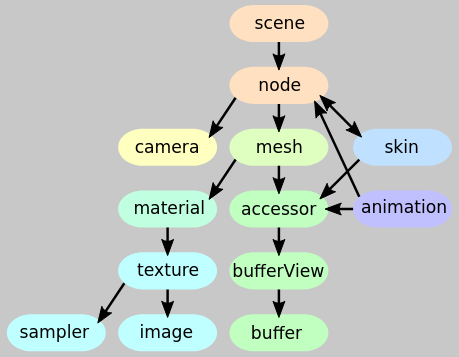
\includegraphics[width=0.80\textwidth]{gltf-structure.png}
	\caption{glTF structure}
\end{figure} \FloatBarrier

\ac{glTF} allows us to not only store an object but entire scenes, with multiple objects each.
These scenes contain allot of data that I will not mention right now or at all. The only thing that
we need right now is that the buffer contains the vertex and index data that we need. This buffer might
refer to a binary data file containing the vertex and index data. It's parent object, the buffer view,
will tell us where the data starts and how long it is. The accessor will tell us the format of the data,
for example if it is a 3D vector or a 2D vector. Then we have a mesh that will contain the accessor
, the material and some additional data like the primitive type. The material will contain the texture that will be used
for the object. The texture will then contain references to the image that the object will use.

We will not worry about how exactly that looks, since there is a library that will do that for us.
The library is called \textit{tinygltf} and is a single header file that we can include in our project.
We will add the \textit{tiny\textunderscore gltf.h}, \textit{json.hpp}, \textit{stb\textunderscore image.h} and
\textit{stb\textunderscore image\textunderscore write.h} header files to our project
and then implement the \textit{loadModel} function.
To add the header files to our project we will have to download them from the
\href{https://github.com/syoyo/tinygltf}{tinygltf} github repository and add it to our project.
To add it you will have to do some digging, since adding a header file to a project is different for each development environment.
You could for example add them to the \textit{/usr/include} directory on linux or add them to the project directory.

Once that is done we can include them in our model file. We do so by defining the \textit{TINYGLTF\textunderscore IMPLEMENTATION},
\textit{STB\textunderscore IMAGE\textunderscore IMPLEMENTATION} and \\
\textit{STB\textunderscore IMAGE\textunderscore WRITE\textunderscore IMPLEMENTATION} macros before including the header file.

\begin{lstlisting}[Language=C++]
//model.cpp
#define TINYGLTF_IMPLEMENTATION
#define STB_IMAGE_IMPLEMENTATION
#define STB_IMAGE_WRITE_IMPLEMENTATION
#include "tiny_gltf.h"
\end{lstlisting}

Now we can implement the \textit{loadModel} function. \textit{tinygltf} provides us with 2 functions that we can use to load in the model data.
One for loading the model from JSON/ASCII files (.gltf) and one from binary files (.glb).
We will use the ASCII function, since most of the time the model data will be stored in ASCII format. Sometimes buffer data will be stored in binary format.
Bevor we can load in model data, we have to create a \textit{tinygltf} model and a \textit{tinygltf} loader. Additionally we need a error string and a warning string.

The loader holds the \textit{LoadASCIIFromFile} function that will load in the model data from a file. It takes in a pointer to the \textit{tinygltf} model
that we will write the data to, the error string that will be filled with an error message if the function fails, the warning string that will be filled with a warning message if one occurs
and finally the path to the model file. The function will return a boolean that indicates if the function was successful or not. If the error string is not empty
we will check if it is empty and debug log the error message. We'll do the same for the warning string and the result of the function.

\begin{lstlisting}[Language=C++]
void Model::Builder::loadModel(const std::string &filepath) {
  tinygltf::Model gltfModel;
  tinygltf::TinyGLTF loader;
  std::string err;
  std::string warn;

  bool result = loader.LoadASCIIFromFile(&gltfModel, &err, &warn, filepath);

  if(!err.empty())
    LOG_ERROR(err);

  if(!warn.empty())
    LOG_WARN(warn);

  if(!result)
    throw std::runtime_error("Failed to load model!");
}
\end{lstlisting}

Next we have to get the vertices and indices from the model data. The model contains a list of meshed that we can iterate over. For each mesh we will access each primitive.
Each primitive has a list of attributes, that define the buffers accessors by index. For example, the vertex aka position buffer might be stored in the 0th accessor. Therfore
the attribute with the key \textit{POSITION} will have the value 0. We will get the accessor by the index and then hangle to the buffer view using the accessors buffer view index.
The buffer view will then give us the buffer that contains the data in binary format. We can then reinterpret cast the binary data to a float pointer. This will give us the vertex data
in a sequential ordered array.

\begin{lstlisting}[Language=C++]
void Model::Builder::loadModel(const std::string &filepath) {
  ...
  for(const auto &mesh : gltfModel.meshes){
    for(const auto &primitive: mesh.primitives){
      const auto &vertexAccessor = gltfModel.accessors[primitive.attributes.find("POSITION")];
      const auto &vertexBufferView = gltfModel.bufferViews[vertexAccessor.bufferView];
      const auto &vertexBuffer = gltfModel.buffers[vertexBufferView.buffer];
      const float *vertexData = reinterpret_cast<const float *>(&vertexBuffer.data[vertexBufferView.byteOffset + vertexAccessor.byteOffset]);
    }
  }
}
\end{lstlisting}

Okay so the vertex data is now a buffer of floats. We will have to convert this buffer to a vector of vertices. But how exactly do we do that?
The vertex data is stored in a sequential array with alternating x, y and z values. We will have to iterate over the vertex data and add the x, y and z values.
as a new Vertex, to our vertices vector.

\begin{lstlisting}[Language=C++]
void Model::Builder::loadModel(const std::string &filepath) {
  ...
  for (size_t i = 0; i < vertexAccessor.count; i++) {                                                                                                                                                 
    vertices.push_back({{vertexData[i * 3], vertexData[i * 3 + 1],                                                                   
        vertexData[i * 3 + 2]}});                                                                                                                                                                                
  }  
}
\end{lstlisting}

Now we do the exact same for the indices data. With the exception that we will get the accessor by the index of the primitive indices attribute and
store each element in the indices vector seperately as a uint32\textunderscore t. Additionally we will have to check if the model has indices, because
not all models have indices. To do so we will check if the primitive has a indices attribute by checking if it is non negative.

\begin{lstlisting}[Language=C++]
  ...
  if(primitive.indices >= 0){
    const auto &indexAccessor = gltfModel.accessors[primitive.indices];
    const auto &indexBufferView =
        gltfModel.bufferViews[indexAccessor.bufferView];
    const auto &indexBuffer = gltfModel.buffers[indexBufferView.buffer];
    const uint32_t *indexData =
        reinterpret_cast<const uint32_t *>(&indexBuffer.data[0]);

    for (size_t i = 0; i < indexAccessor.count; i++) {
      indices.push_back(indexData[i]);
    }
  }
\end{lstlisting}

\subsection{Model construction}

Now that we have the model data, we can construct the model. To do so we will add a static \textit{createModelFromFile} function to the model class that will take the device and the path to the model file as parameters.
This function will create a builder object and call the \textit{loadModel} function. Then it will return a unique pointer to the model object.
For the model, I've found a simple cube model online from this \href{https://sketchfab.com/3d-models/epic-simple-cube-3a180582490b4395bc6384ea2bb740aa}{sketchfab} website.
I've downloaded the model and placed it in the models directory. Full credit goes to German\textunderscore Martian \cite{German_Martian} for creating the model.
The model will be a shared pointer to the model class and will be created by passing the device and the builder object to the model constructor.
The reason we use a shared pointer is because we will have to pass the model to the renderer class and we do not want to copy the model data.

\begin{lstlisting}[Language=C++]
std::unique_ptr<Model> Model::createModelFromFile(Device &device,
                                                  const std::string &filepath) {
  Builder builder = {};
  builder.loadModel(filepath);

  return std::make_unique<Model>(device, builder);
}
\end{lstlisting}

The \texit{createModelFromFile} function will be called in a \textit{loadGameObjects} function in the Application classes constructor.

\begin{lstlisting}[Language=C++]
App::App() {
  loadGameObjects();
}

void App::loadGameObjects() {
 model  = Model::createModelFromFile(device, "models/cube/scene.gltf");
}
\end{lstlisting}

\subsection{Buffer usage}

We've created the vertex and index buffers and they are located on the GPU. But we still haven't told the GPU to use them.
To do so we have to bind each models buffers to the graphics pipeline and then draw the model using the \textit{vkCmdDrawIndexed} function,
which will ignore the predefined primitive topology and use the indices to draw the model.

We will add a \textit{bind} function to the model class that will take the command buffer as a parameter and bind the vertex and index buffers to the graphics pipeline.
We'll call this function while recording the command buffer, after binding the pipeline. Inside the \textit{bind} function we will call the \textit{vkCmdBindVertexBuffers}
function, which allows us to bind multiple vertex buffers to the graphics pipeline. Because it takes an array of buffers and offsets, we will have to add our vertex buffer
to an array and create an additional array for the offsets.

\begin{lstlisting}[Language=C++]
void Model::bind(VkCommandBuffer commandBuffer) {
  VkBuffer vertexBuffers[] = {vertexBuffer->getBuffer()};
  VkDeviceSize offsets[] = {0};
  vkCmdBindVertexBuffers(commandBuffer, 0, 1, vertexBuffers, offsets);
}
\end{lstlisting}

To understand, what the \textit{vkCmdBindVertexBuffers} function does, we have to take a look our graphics pipeline.
The graphics pipeline has a vertex input state that defines the format and the location of the vertex data.
The vertex input state needs a vertex buffer binding description, which will define the stride aka the size of one vertex and the input rate.
The input rate will define how the data is read from the buffer.
In our case we will use the \textit{VK\textunderscore VERTEX\textunderscore INPUT\textunderscore RATE\textunderscore VERTEX} to indicate that
we will move to the next vertex after each vertex. Otherwise we could use the \textit{VK\textunderscore VERTEX\textunderscore INPUT\textunderscore RATE\textunderscore INSTANCE}
to indicate that we will move to the next vertex after each instance.
It also needs a vertex attribute description, which will define the format of the vertex data. This struct will define the binding, the location, the format and the format.
The binding is used to link the vertex buffer binding description to the corresponding vertex attribute description. The location is used to link the vertex attribute description to the shader
and the format is used to define if the data is a float, a vec2, a vec3 or a vec4. We will need two vertex attribute descriptions, one for each vertex attribute.
Let's go ahead and add two functions to the Vertex struct that will return the binding description and the attribute descriptions.

\begin{lstlisting}[Language=C++]
//model.hpp
struct Vertex {
  glm::vec3 position{};
  glm::vec3 color{};

  static std::vector<VkVertexInputBindingDescription> getBindingDescriptions();
  static std::vector<VkVertexInputAttributeDescription> getAttributeDescriptions();
};
\end{lstlisting}

\begin{lstlisting}[Language=C++]
//model.cpp
std::vector<VkVertexInputBindingDescription> Vertex::getBindingDescriptions() {
  std::vector<VkVertexInputBindingDescription> bindingDescriptions(0);
  bindingDescriptions[0].binding = 0;
  bindingDescriptions[0].stride = sizeof(Vertex);
  bindingDescriptions[0].inputRate = VK_VERTEX_INPUT_RATE_VERTEX;

  return bindingDescription;
}
\end{lstlisting}

For the attribute descriptions we will have to define the location of the vertex data. We will use the location 0 for the position and the location 1 for the color.
Both the position and color will be a vec3, so we will use the \textit{VK\textunderscore FORMAT\textunderscore R32G32B32\textunderscore SFLOAT} format.
Even tho the position is not a RGB value, we will use the RGB format, because it uses 3 floats.
The binding will be 0 for both, because we only have one binding description and the offset will be the result of the \textit{offsetof} function for the position and color.
The \textit{offsetof} calculates the offset of one attribute in a struct.

\begin{lstlisting}[Language=C++]
std::vector<VkVertexInputAttributeDescription> Vertex::getAttributeDescriptions() {
  std::vector<VkVertexInputAttributeDescription> attributeDescriptions = {};
  attributeDescriptions.push_back({0, 0, VK_FORMAT_R32G32B32_SFLOAT, offsetof(Vertex, position)});
  attributeDescriptions.push_back({0, 1, VK_FORMAT_R32G32B32_SFLOAT, offsetof(Vertex, color)});

  return attributeDescriptions;
}
\end{lstlisting}

Now we will have to add the vertex input state to the graphics pipeline.

\begin{lstlisting}[Language=C++]
void Pipeline::createGraphicsPipeline(const std::string &vertPath, const std::string &fragPath, const PipelineConfigInfo &configInfo) {
  ...
  auto bindingDescriptions = Model::Vertex::getBindingDescriptions();
  auto attributeDescriptions = Model::Vertex::getAttributeDescriptions();

  VkPipelineVertexInputStateCreateInfo vertexInputInfo = {};
  vertexInputInfo.sType = VK_STRUCTURE_TYPE_PIPELINE_VERTEX_INPUT_STATE_CREATE_INFO;
  vertexInputInfo.vertexBindingDescriptionCount = static_cast<uint32_t>(bindingDescriptions.size());
  vertexInputInfo.vertexAttributeDescriptionCount = static_cast<uint32_t>(attributeDescriptions.size());
  vertexInputInfo.pVertexBindingDescriptions = bindingDescriptions.data();
  vertexInputInfo.pVertexAttributeDescriptions = attributeDescriptions.data();
}
\end{lstlisting}

Great! Now we have bound the vertex buffer to the graphics pipeline, specificly to the input assembler stage.
But we have still not bound the index buffer to the graphics pipeline. To do so we will check if the model has an index buffer and if it does, we will call the \textit{vkCmdBindIndexBuffer}
function. Since we can not bind multiple index buffers to the graphics pipeline at once, we can simple pass in the index buffer, the offset and the index type to the function.
The index type is used to define how big the indices are. We will use the \textit{VK\textunderscore INDEX\textunderscore TYPE\textunderscore UINT32} type, because we are using 32 bit indices.

\begin{lstlisting}[Language=C++]
void Model::bind(VkCommandBuffer commandBuffer) {
  VkBuffer vertexBuffers[] = {vertexBuffer->getBuffer()};
  VkDeviceSize offsets[] = {0};
  vkCmdBindVertexBuffers(commandBuffer, 0, 1, vertexBuffers, offsets);

  if(hasIndexBuffer)
    vkCmdBindIndexBuffer(commandBuffer, indexBuffer->getBuffer(), 0, VK_INDEX_TYPE_UINT32);
}
\end{lstlisting}

Alright we have everything set up, so that we can draw the model. Currently we are using the \textit{vkCmdDraw} function to draw the model.
This function does not take indices into account and will just draw the vertices in the order they are stored in the vertex buffer.
To use the indices, we will have to use the \textit{vkCmdDrawIndexed} function. This function will take
the command buffer, the index count, the instance count, the first index and the vertex offset as parameters..
The instance count tells us how many time the model will be drawn.

We will add a \textit{draw} function to the model class that will take the command buffer as a parameter and call the \textit{vkCmdDrawIndexed} function,
if the model has an index buffer. If it does not have an index buffer, we will call the \textit{vkCmdDraw} function.

\begin{lstlisting}[Language=C++]
void Model::draw(VkCommandBuffer commandBuffer) {
  if(hasIndexBuffer)
    vkCmdDrawIndexed(commandBuffer, indexCount, 1, 0, 0, 0);
  else
    vkCmdDraw(commandBuffer, vertexCount, 1, 0, 0);
}
\end{lstlisting}

To call the bind and draw command we will have to add a \textit{renderGameObjects} function to the render system class and call it in the \textit{run} function
after the \textit{recordCommandBuffer} function. We will have to pass the command buffer and the model to the \textit{renderGameObjects} function. Since we can only render
objects while the render pass is active, we will have to extract the \textit{vkCmdEndRenderPass} function from the \textit{recordCommandBuffer} function and call it after
the \textit{renderGameObjects} function.

\begin{lstlisting}[Language=C++]
void RenderSystem::renderGameObjects(VkCommandBuffer commandBuffer, std::shared_ptr<Model> model) {
  model->bind(commandBuffer);
  model->draw(commandBuffer);
}

void RenderSystem::endRenderPass(VkCommandBuffer commandBuffer) {
  vkCmdEndRenderPass(commandBuffer);
}
\end{lstlisting}

\begin{lstlisting}[Language=C++]
void App::run() {
  while (!window.shouldClose()) {
    glfwPollEvents();

    if (auto commandBuffer = renderSystem.beginFrame()) {
      renderSystem.recordCommandBuffer(commandBuffer);
      renderSystem.renderGameObjects(commandBuffer, model);
      renderSystem.endRenderPass(commandBuffer);
      renderSystem.endFrame();
    }
  }
}
\end{lstlisting}

\subsection{Vertex Shader}

Currently we are only using the vertices in the input assembler stage. We are not using the vertices in the vertex shader.
We can access them through a layout qualifier. The layout qualifier holds the locations of the vertex datas position and color.
These locations are the ones we defined in the \textit{getAttributeDescriptions} function and to access them we will use the in keyword.

Then, from these vec3's we can pass the position to the gl\textunderscore Position variable and add the w component to it.
The color will be passed to the fragment shader by passing it to an out variable called fragColor. This out variable will be passed to the next pipeline stage.

\begin{lstlisting}[Language=C++]
#version 460

layout(location = 0) in vec3 inPosition;
layout(location = 1) in vec3 inColor;

layout(location = 0) out vec3 fragColor;

void main() {
	gl_Position = vec4(inPosition, 1.0);
  fragColor = inColor;
}
\end{lstlisting}

To use the \textit{fragColor} variable in the fragment shader we will have to use the in keyword to define the variable as an input variable
and then pass it to a vec 4 out variable that will be outputted to the framebuffer. This will ensure that each fragment will be colored with the color of the vertex.

\begin{lstlisting}[Language=C++]
#version 460

layout (location = 0) in vec3 fragColor;

layout (location = 0) out vec4 outColor;

void main() {
  outColor = vec4(fragColor, 1.0);
}
\end{lstlisting}

Let's run our application and see if the cube is rendered. Hmm, the cube is not rendered. Let's take a look at our model data.
Debuging the vertices, we see that our model is a cube ranging from -1 to 1 in all directions. But since every vertex outside of
our \ac{CVV} will be clipped, including the ones that are at the edge of the \ac{CVV}, we will have to move the cube in front of the camera.
This will also be the perfect timing to add a view and a projection matrix to our vertex shader, making our cube be rendered in perspective.

\section{Push Constants}

Push constants are a way to pass data to the shader. They are a small amount of memory that is pushed onto the \ac{GPU} when the command buffer is recorded.
These constants are then accessible in the shader but not mutable. They are a way to pass data to the shader that is constant for the entire draw call.
We will use push constants to move and rotate the cube in the vertex shader via a transformation matrix.

\subsection{Game Objects}

Before we start pushing constants we will make a few changes to our code. We will add a new class called \textit{GameObject} that will hold the model and the transform of the object
The transform will be a struct holding the position, the rotation and the scale of the object and also some functions to turn the data into helpful matrices.
Each game object will have a unique id that will be used to identify the object. We will also add a static \textit{createGameObject} function that
sets the id of the object to the next id and returns the object. Let's also add a getter function for the id.

\begin{lstlisting}[Language=C++]
//game_object.hpp
struct Transform {
		glm::vec3 position{};
		glm::vec3 rotation{};
		glm::vec3 scale{1.0f, 1.0f, 1.0f};

		glm::mat4 mat4();
	};

class GameObject {
public:
  using id_t = unsigned int;

  static GameObject createGameObject(){
      static id_t currentId = 0;
      return GameObject{currentId++};
    }

  GameObject(const GameObject &) = delete;
  GameObject &operator=(const GameObject &) = delete;
  GameObject(GameObject &&) = default;
  GameObject &operator=(GameObject &&) = default;

  id_t getId() const { return id; }

  std::shared_ptr<Model> model{};
  Transform transform{};

private:
  GameObject(id_t id) : id{id} {}

  id_t id;
};
\end{lstlisting}

Now we will have to apply our math knowledge to combine the position, rotation and scale into a transformation matrix.
Before, we only had each of these matrices seperate. Now we will have to combine them into one matrix.
One important thing to note is that the order of the matrices is important. This comes from the fact that, when we use matrices to transform objects,
we are actually transforming the coordinate system. For example, if we first move an object and then rotate it, the object will rotate around the origin,
which will move the object to a different position.

The order of the matrices is as follows: scale, rotate, translate. Matrices are multiplied from right to left. So when we tranform an object we will have the following equation:

\begin{equation}
	\begin{aligned}
		\vec{v'} = T_{translate} \cdot T_{rotate} \cdot T_{scale} \cdot \vec{v}
	\end{aligned}
\end{equation}

We can simply cut out the vector v and multiply the matrices together to get the transformation matrix. But wait, we have 3 different ways to rotate an object.
We can rotate it around the x, y or z axis. We will have to create a rotation matrix for each axis and then multiply them together to get the final rotation matrix.
There are multiple ways to rotate an object, but the most common way is to use the Euler angles. There are 2 types of Euler angles, porper Euler angles and Tait-Bryan angles.
The difference between the two is that proper Euler angles use the same axis for the first and third rotation, while Tait-Bryan angles use 3 distinct axis.
The most common way in game development is to use the YXZ Tait-Bryan angles. This means that we first rotate the object around the y axis, then around the x axis and then around the z axis.
Therefor the full transformation matrix will be assembled like this:

\begin{equation}
	\begin{aligned}
		\begin{bmatrix}
			1 & 0 & 0 & t_x \\
			0 & 1 & 0 & t_y \\
			0 & 0 & 1 & t_z \\
			0 & 0 & 0 & 1
		\end{bmatrix}
		\cdot
		\begin{bmatrix}
			\cos(\theta_z)  & \sin(\theta_z) & 0 & 0 \\
			-\sin(\theta_z) & \cos(\theta_z) & 0 & 0 \\
			0               & 0              & 1 & 0 \\
			0               & 0              & 0 & 1
		\end{bmatrix}
		\cdot
		\begin{bmatrix}
			1 & 0               & 0              & 0 \\
			0 & \cos(\theta_x)  & \sin(\theta_x) & 0 \\
			0 & -\sin(\theta_x) & \cos(\theta_x) & 0 \\
			0 & 0               & 0              & 1
		\end{bmatrix}
		\\
		\cdot
		\begin{bmatrix}
			\cos(\theta_y) & 0 & -\sin(\theta_y) & 0 \\
			0              & 1 & 0               & 0 \\
			\sin(\theta_y) & 0 & \cos(\theta_y)  & 0 \\
			0              & 0 & 0               & 1
		\end{bmatrix}
		\cdot
		\begin{bmatrix}
			s_x & 0   & 0   & 0 \\
			0   & s_y & 0   & 0 \\
			0   & 0   & s_z & 0 \\
			0   & 0   & 0   & 1
		\end{bmatrix}
	\end{aligned}
\end{equation}

Okay, we'll go through this step by step. First we will calculate the Tait-Bryan rotation matrix by multiplying the rotation matrices for the x, y and z axis
in the y, x, z order.

\begin{equation}
	\begin{aligned}
		\begin{bmatrix}
			\cos(\theta_y)  & 0 & \sin(\theta_y) & 0 \\
			0               & 1 & 0              & 0 \\
			-\sin(\theta_y) & 0 & \cos(\theta_y) & 0 \\
			0               & 0 & 0              & 1
		\end{bmatrix}
		\cdot
		\begin{bmatrix}
			1 & 0              & 0               & 0 \\
			0 & \cos(\theta_x) & -\sin(\theta_x) & 0 \\
			0 & \sin(\theta_x) & \cos(\theta_x)  & 0 \\
			0 & 0              & 0               & 1
		\end{bmatrix}
		=
		\fontsize{8}{12}\selectfont
		\begin{bmatrix}
			\cos(\theta_y)  & \sin(\theta_y) \sin(\theta_x) & \sin(\theta_y) \cos(\theta_x) & 0 \\
			0               & \cos(\theta_x)                & -\sin(\theta_x)               & 0 \\
			-\sin(\theta_y) & \cos(\theta_y)\sin(\theta_x)  & \cos(\theta_y) \cos(\theta_x) & 0 \\
			0               & 0                             & 0                             & 1
		\end{bmatrix}
	\end{aligned}
\end{equation}

\begin{equation}
	\begin{center}
		R \cdot
		\begin{bmatrix}
			\cos(\theta_z) & -\sin(\theta_z) & 0 & 0 \\
			\sin(\theta_z) & \cos(\theta_z)  & 0 & 0 \\
			0              & 0               & 1 & 0 \\
			0              & 0               & 0 & 1
		\end{bmatrix}
		\\
		=
		\fontsize{8}{12}\selectfont
		\begin{bmatrix}
			\cos(\theta_y) \cos(\theta_z) + \sin(\theta_y) \sin(\theta_x) \sin(\theta_z) & \sin(\theta_y) \sin(\theta_x) \cos(\theta_z) - \sin(\theta_z) \cos(\theta_y) & \sin(\theta_y) \cos(\theta_x) & 0 \\
			\cos(\theta_x) \sin(\theta_z)                                                & \cos(\theta_x) \cos(\theta_z)                                                & -\sin(\theta_x)               & 0 \\
			\cos(\theta_y) \sin(\theta_x) \sin(\theta_z) - \sin(\theta_y) \cos(\theta_z) & \sin(\theta_y) \sin(\theta_z) + \cos(\theta_y) \sin(\theta_x) \cos(\theta_z) & \cos(\theta_y) \cos(\theta_x) & 0 \\
			0                                                                            & 0                                                                            & 0                             & 1
		\end{bmatrix}
	\end{center}
\end{equation}

Now we need to multiply the translation matrix with the rotation matrix and then multiply the result with the scale matrix.

\begin{equation}
	\begin{center}
		\begin{bmatrix}
			1 & 0 & 0 & t_x \\
			0 & 1 & 0 & t_y \\
			0 & 0 & 1 & t_z \\
			0 & 0 & 0 & 1
		\end{bmatrix}
		\cdot
		M_{rotation}
		\\
		\fontsize{8}{12}\selectfont
		=
		\begin{bmatrix}
			\cos(\theta_y) \cos(\theta_z) + \sin(\theta_y) \sin(\theta_x) \sin(\theta_z) & \sin(\theta_y) \sin(\theta_x) \cos(\theta_z) - \sin(\theta_z) \cos(\theta_y) & \sin(\theta_y) \cos(\theta_x) & t_x \\
			\cos(\theta_x) \sin(\theta_z)                                                & \cos(\theta_x) \cos(\theta_z)                                                & -\sin(\theta_x)               & t_y \\
			\cos(\theta_y) \sin(\theta_x) \sin(\theta_z) - \sin(\theta_y) \cos(\theta_z) & \sin(\theta_y) \sin(\theta_z) + \cos(\theta_y) \sin(\theta_x) \cos(\theta_z) & \cos(\theta_y) \cos(\theta_x) & t_z \\
			0                                                                            & 0                                                                            & 0                             & 1
		\end{bmatrix}
	\end{center}
\end{equation}

\begin{equation}
	\begin{center}
		R \cdot
		\begin{bmatrix}
			s_x & 0   & 0   & 0 \\
			0   & s_y & 0   & 0 \\
			0   & 0   & s_z & 0 \\
			0   & 0   & 0   & 1
		\end{bmatrix}
		=
		\\
		\fontsize{8}{12}\selectfont
		\begin{bmatrix}
			s_x (\cos(\theta_y) \cos(\theta_z) + \sin(\theta_y) \sin(\theta_x) \sin(\theta_z)) & s_y \cdot (\sin(\theta_y) \sin(\theta_x) \cos(\theta_z) - \sin(\theta_z) \cos(\theta_y)) & s_z \sin(\theta_y) \cos(\theta_x)) & t_x \\
			s_x \cos(\theta_x) \sin(\theta_z)                                                  & s_y \cos(\theta_x) \cos(\theta_z)                                                        & s_z (-\sin(\theta_x))              & t_y \\
			s_x (\cos(\theta_y) \sin(\theta_x) \sin(\theta_z) - \sin(\theta_y) \cos(\theta_z)) & s_y \cdot (\sin(\theta_y) \sin(\theta_z) + \cos(\theta_y) \sin(\theta_x) \cos(\theta_z)) & s_z \cos(\theta_y) \cos(\theta_x)  & t_z \\
			0                                                                                  & 0                                                                                        & 0                                  & 1
		\end{bmatrix}
	\end{center}
\end{equation}

Great! That's our combined transformation matrix. We could have just used some glm functions to get the same result, but calculating it by hand is a good way to understand how matrices work and is
also a more performant way to have the transformation matrix already calculated, since we would have to perform theses calculations in each frame. Let's add the \textit{mat4} function to the Transform struct.
First we will get all the sin and cos values for the rotation angles and then we will return a glm::mat4 with the calculated values.

\begin{lstlisting}
//game_object.cpp
glm::mat4 mat4(){
  const float c1 = glm::cos(rotation.y);
  const float s1 = glm::sin(rotation.y);
  const float c2 = glm::cos(rotation.x);
  const float s2 = glm::sin(rotation.x);
  const float c3 = glm::cos(rotation.z);
  const float s3 = glm::sin(rotation.z);
  return glm::mat4{{
                       scale.x * (c1 * c3 + s1 * s2 * s3),
                       scale.x * c2 * s3,
                       scale.x * (c1 * s2 * s3 - s1 * c3),
                       0.f,
                   },
                   {
                       scale.y * (s1 * s2 * c3 - s3 * c1),
                       scale.y * c2 * c3,
                       scale.y * (s1 * s3 + c1 * s2 * c3),
                       0.f,
                   },
                   {
                       scale.z * s1 * c2,
                       scale.z * -s2,
                       scale.z * c1 * c2,
                       0.f,
                   },
                   {position.x, position.y, position.z, 1.f}};
}
\end{lstlisting}

Now that we have to create a GameObject, for our model and set the position and scale of the object.
To do so we will modify the \textit{loadGameObjects} function in the Application class to create a GameObject, set the model and the position and scale of the object
and push it to a vector of GameObjects.

\begin{lstlisting}[Language=C++]
void App::loadGameObjects() {
  std::shared_ptr<Model> cubeModel =
      Model::createModelFromFile(device, "models/cube/scene.gltf");
  GameObject cube = GameObject::createGameObject();
  cube.model = cubeModel;

  gameObjects.push_back(std::move(cube));
}
\end{lstlisting}

Accordingly we will have to modify the \textit{renderGameObjects} function in the RenderSystem class to take in a vector of GameObjects and bind and draw each object.

\begin{lstlisting}[Language=C++]
void RenderSystem::renderGameObjects(VkCommandBuffer commandBuffer, const std::vector<GameObject> &gameObjects) {
  for(const auto &gameObject : gameObjects){
    gameObject.model->bind(commandBuffer);
    gameObject.model->draw(commandBuffer);
  }
}
\end{lstlisting}

\begin{lstlisting}[Language=C++]
void App::run() {
  while (!window.shouldClose()) {
    glfwPollEvents();

    if (auto commandBuffer = renderSystem.beginFrame()) {
      renderSystem.recordCommandBuffer(commandBuffer);
      renderSystem.renderGameObjects(commandBuffer, gameObjects);
      renderSystem.endRenderPass(commandBuffer);
      renderSystem.endFrame();
    }
  }
}
\end{lstlisting}

\subsection{Push Constant Data}

Now we can start pushing the transformation matrix to the shader. To do so we will have to add a new struct to the RenderSystem class that will hold the transformation matrix.
The transformation matrix will be a glm::mat4 called modelMatrix. The reason we need a new struct is because we will have to provide the size of the push constant data to the pipeline,
when we push the data to the shader.

\begin{lstlisting}[Language=C++]
//render_system.cpp
struct PushConstantData {
  glm::mat4 modelMatrix;
};
\end{lstlisting}

We will also have to adjust our pipeline layout, so that it knows that we will use push constants. For that case we will have to add a push constant range to the pipeline layout,
that will define the size of the push constant data and the shader stages that will use the push constants. We will use the vertex shader stage for now.

\begin{lstlisting}[Language=C++]
void RenderSystem::createPipelineLayout(
    VkDescriptorSetLayout descriptorSetLayout) {
  VkPushConstantRange pushConstantRange = {};
  pushConstantRange.stageFlags = VK_SHADER_STAGE_VERTEX_BIT;
  pushConstantRange.offset = 0;
  pushConstantRange.size = sizeof(PushConstantData);
  std::vector<VkDescriptorSetLayout> layouts{descriptorSetLayout};


  VkPipelineLayoutCreateInfo pipelineLayoutInfo = {};
  pipelineLayoutInfo.sType = VK_STRUCTURE_TYPE_PIPELINE_LAYOUT_CREATE_INFO;
  pipelineLayoutInfo.setLayoutCount =
      0; // static_cast<uint32_t>(layouts.size());
  pipelineLayoutInfo.pSetLayouts = nullptr; // layouts.data();
  pipelineLayoutInfo.pushConstantRangeCount = 1;
  pipelineLayoutInfo.pPushConstantRanges = &pushConstantRange;

  if (vkCreatePipelineLayout(device.device(), &pipelineLayoutInfo, nullptr,
                             &pipelineLayout) != VK_SUCCESS)
    throw std::runtime_error("Failed to create pipeline layout!");
}
\end{lstlisting}

\subsection{Pushing the data}

Inside our \textit{renderGameObjects} function we will push the push constant data to the shader. To do so we will create a PushConstantData object and provide its modelMatrix with the result from the mat4 function of the transform object.
Then have to call the \textit{vkCmdPushConstants} function. This function will take the command buffer, the pipeline layout, the shader stages we will push to, the offset and the size of the push constant data and the data itself.
Vulkan requires GPU's to allow a minimum of 128 bytes for push constants, which is exactly the size of two 4x4 matrices. This is obviously not much data, but it is enough to pass our model matrix to the shader.
The data will be pushed to the vertex shader, because we will use the model matrix to transform the vertices. The offset can later be used to push different matrices to different shader stages.

\begin{lstlisting}[Language=C++]
void RenderSystem::renderGameObjects(VkCommandBuffer commandBuffer,
                                     std::vector<GameObject> &gameObjects) {
  for (GameObject &gameObject : gameObjects) {
    PushConstantData push{};
    push.modelMatrix = gameObject.transform.mat4();

    vkCmdPushConstants(commandBuffer, pipelineLayout,
                       VK_SHADER_STAGE_VERTEX_BIT,
                       0, sizeof(PushConstantData), &push);

    gameObject.model->bind(commandBuffer);
    gameObject.model->draw(commandBuffer);
  }
}
\end{lstlisting}

\subsection{Transformation in the shader}

We can now access the push constants in the shader via a layout qualifier called \textit{push\textunderscore constant}. This layout qualifier will be uniform, which means that it will be constant for the entire draw call,
aka for each vertex. The created Object will be called Push and has to have the same structure as the PushConstantData struct. We will then access the modelMatrix and multiply it with the vertex position.

\begin{lstlisting}[Language=C++]
#version 460
layout(location = 0) in vec3 inPosition;
layout(location = 1) in vec3 inColor;

layout(location = 0) out vec3 fragColor;

layout(push_constant) uniform Push {
  mat4 modelMatrix;
} push;

void main() {
  gl_Position = push.modelMatrix * vec4(inPosition, 1.0);
  fragColor = inColor;
}
\end{lstlisting}

\subsection{Final Result}

We can now specify a position rotation and scale for our game object and render it. Let's try by setting the position of the cube to (0, 0, 2) and the scale to (0.5, 0.5, 0.5).
We will also rotate the cube around the z axis by 45 degrees and around the y axis by 30 degrees, which we will have to provide as radians.
The final result should be a rotated and scaled square in the center of the screen.

\begin{lstlisting}[Language=C++]
void App::loadGameObjects() {
  std::shared_ptr<Model> cubeModel =
      Model::createModelFromFile(device, "models/cube/scene.gltf");
  GameObject cube = GameObject::createGameObject();
  cube.model = cubeModel;
  cube.transform.position = {0.f, 0.f, 2.f};
  cube.transform.scale = {0.5f, 0.5f, 0.5f};
  cube.transform.rotation = {0.f, glm::radians(30.f), glm::radians(45.f)};

  gameObjects.push_back(std::move(cube));
}
\end{lstlisting}

\begin{figure}[htbp]
	\centering
	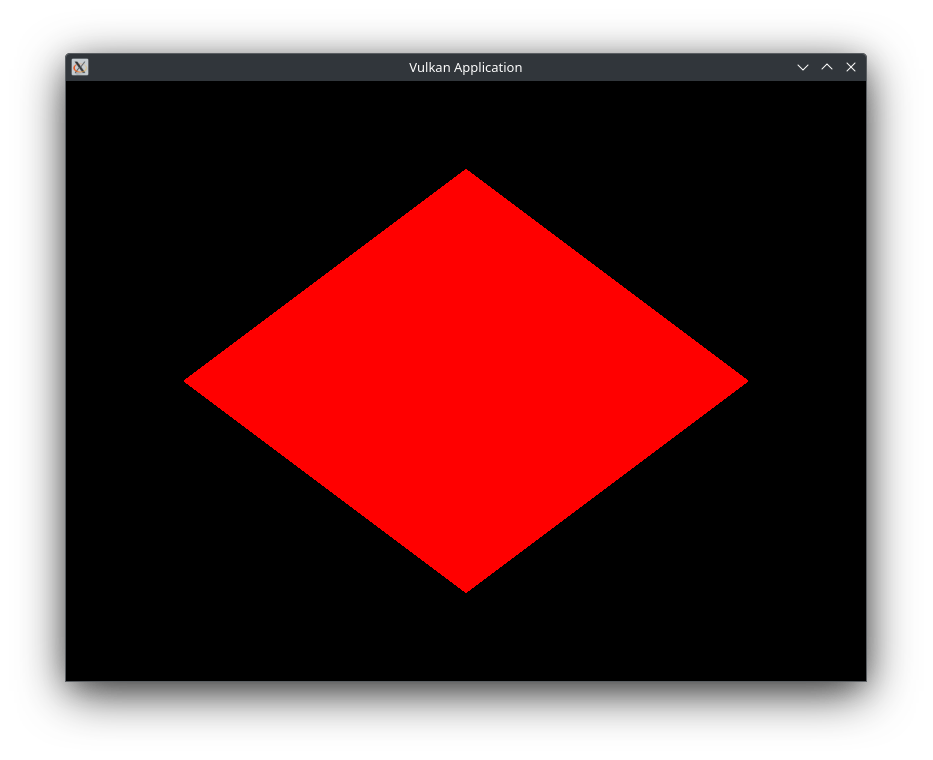
\includegraphics[width=0.8\textwidth]{images/rotated_cube.png}
	\caption{Rotated and scaled cube}
\end{figure}

Currently we are rendering the cube in orthographic projection. We will have to create the projection view matrix and pass it to the shader to render the cube in perspective.
Since this matrix changes very often, we will not use push constants to pass the matrix to the shader. Instead we will use a uniform buffer object.

\section{Uniform Buffers}

Uniform buffers are a way to pass data to a shader that is persistent for the entire draw call and is identical for each invocation of the shader.
These \ac{UBO} also have the advantage that they can hold more data than push constants. For now, we will use a uniform buffer to pass the perspective projection matrix to the shader,
to render the cube in perspective.

First we will have to create one \ac{UBO} for each frame in flight in our \textit{run} function. To create the buffer we can use our Buffer class.
If you remember, to create a Buffer instance we have to provide the device, the size of the buffer, the usage of the buffer and the properties of the buffer.
The size of the buffer will be the size of the projection view matrix. While we could simply use the size of the matrix, we will look ahead and add a struct that will hold all of the
global \ac{UBO} data.

\begin{lstlisting}[Language=C++]
//app.cpp
namespace engine {
  struct GlobalUbo{
    glm::mat4 projectionView{1.f};
  };
  ...
}
\end{lstlisting}

We called the matrix projectionView, because it will later hold the combined projection and view matrix. For now we will just use the projection matrix.
Now we can just use the sizeof function to get the size of the GlobalUbo struct. The usage of the buffer will be \textit{VK\textunderscore BUFFER\textunderscore USAGE\textunderscore UNIFORM\textunderscore BUFFER\textunderscore BIT}.
For the properties of the buffer we will just use the \\ \textit{VK\textunderscore MEMORY\textunderscore PROPERTY\textunderscore HOST\textunderscore VISIBLE\textunderscore BIT}
But wait a second, we previously used one staging buffer and one device local buffer. Why are we only using one buffer and why are we not using the \textit{VK\textunderscore MEMORY\textunderscore PROPERTY\textunderscore HOST\textunderscore COHERENT\textunderscore BIT} property?

The reason we used a staging buffer when creating the vertex and index buffer is because we had to copy potentially large and mostly static data to the device.
Therefore, copying the data to the more performant device local memory is a good idea. But in the case of the \ac{UBO} we will have to update the data every frame.
Additionly, the data is not that large, so the process of copying the data to the device local memory would be a waste of time and memory.

\begin{lstlisting}[Language=C++]
void App::run() {
  std::vector<std::unique_ptr<Buffer>> uboBuffers(SwapChain::MAX_FRAMES_IN_FLIGHT);
  for (int i = 0; i < uboBuffers.size(); i++) {
    uboBuffers[i] = std::make_unique<Buffer>(
        device, sizeof(GlobalUbo), 1, VK_BUFFER_USAGE_UNIFORM_BUFFER_BIT,
        VK_MEMORY_PROPERTY_HOST_VISIBLE_BIT);
  }

  while (!window.shouldClose()) {
    glfwPollEvents();

    if (auto commandBuffer = renderSystem.beginFrame()) {
      renderSystem.recordCommandBuffer(commandBuffer);
      renderSystem.renderGameObjects(commandBuffer, gameObjects);
      renderSystem.endRenderPass(commandBuffer);
      renderSystem.endFrame();
    }
  }
}
\end{lstlisting}

After creation of the buffer we will have to map the memory of the buffer to the host memory. This will allow us to write data to the buffer.

\begin{lstlisting}[Language=C++]
void App::run() {
  ...
  for (int i = 0; i < uboBuffers.size(); i++) {
    uboBuffers[i] = std::make_unique<Buffer>(
        device, sizeof(GlobalUbo), 1, VK_BUFFER_USAGE_UNIFORM_BUFFER_BIT,
        VK_MEMORY_PROPERTY_HOST_VISIBLE_BIT);
    uboBuffers[i]->map();
  }
  ...
}
\end{lstlisting}

Now that we have the mapped memory we can write the perspective projection matrix to the buffer with the \textit{writeToBuffer} function.
Currently our matrix is a 4x4 identity matrix, which is not a perspective projection matrix. We will add a camera object in a second that will handle the perpective projection matrix.
Let's just create a GlobalUbo object and write it to the buffer for now. Since the data changes every frame, we will have to write the data to the buffer every frame. But we
have mutliple buffers, so we will have to get the current frame index and write the data to the buffer of the same index.

\begin{lstlisting}[Language=C++]
void App::run() {
  ...
  while (!window.shouldClose()) {
    glfwPollEvents();

    if (auto commandBuffer = renderSystem.beginFrame()) {
      int frameIndex = renderSystem.getFrameIndex();

      GlobalUbo ubo{};
      uboBuffers[frameIndex]->writeToBuffer(&ubo);

      renderSystem.recordCommandBuffer(commandBuffer);
      renderSystem.renderGameObjects(commandBuffer, gameObjects);
      renderSystem.endRenderPass(commandBuffer);
      renderSystem.endFrame();
    }
  }
}
\end{lstlisting}

You might remember me saying that when we don't use device local memory we might have to synchronize the memory ourselves. This is the case here.
When we map our buffer we basically link host memory to device memory. This means that we write the data to the CPU's cache.
When we use non-coherent memory, the changes we make to the CPU cache are not automatically written to the device memory, because the GPU does not have access to the CPU cache.
To do this we will have to flush the memory, which will write the data to the GPU. We will add a \textit{flush} function to the Buffer class that will flush the memory of the buffer.

\begin{lstlisting}[Language=C++]
void App::run() {
  ...
  while (!window.shouldClose()) {
    glfwPollEvents();

    if (auto commandBuffer = renderSystem.beginFrame()) {
      int frameIndex = renderSystem.getFrameIndex();

      GlobalUbo ubo{};
      uboBuffers[frameIndex]->writeToBuffer(&ubo);
      uboBuffers[frameIndex]->flush();

      renderSystem.recordCommandBuffer(commandBuffer);
      renderSystem.renderGameObjects(commandBuffer, gameObjects);
      renderSystem.endRenderPass(commandBuffer);
      renderSystem.endFrame();
    }
  }
}
\end{lstlisting}

The \textit{flush} function will use the \textit{vkFlushMappedMemoryRanges} function to flush the memory of the buffer.
It takes the device, the number of memory ranges, the memory ranges and the result as parameters. The memory range will be a VkMappedMemoryRange struct
that will describe CPU cache memory that we want to flush. We will have to provide the memory of the buffer, the offset and the size of the memory.
We will also add optional parameters to the \textit{writeToBuffer} function that will allow us to specify the size and the offset of the data we want to write to the buffer.
As default values we will use \textit{VK\textunderscore WHOLE\textunderscore SIZE} and 0.

\begin{lstlisting}[Language=C++]
//buffer.hpp
...
public:
  void flush(VkDeviceSize size = VK_WHOLE_SIZE, VkDeviceSize offset = 0);
...
\end{lstlisting}

\begin{lstlisting}[Language=C++]
//buffer.cpp
...
void Buffer::flush(VkDeviceSize size, VkDeviceSize offset) {
  VkMappedMemoryRange memoryRange = {};
  memoryRange.sType = VK_STRUCTURE_TYPE_MAPPED_MEMORY_RANGE;
  memoryRange.size = size;
  memoryRange.offset = offset;
  memoryRange.memory = bufferMemory;

  vkFlushMappedMemoryRanges(device.device(), 1, &memoryRange);
}
...
\end{lstlisting}

\subsection{Descriptors}

Uniform buffers are provided to the Pipeline via descriptor sets. A Descriptor set is simply a collection of descriptions of resources.
These descriptions are importent for the Pipeline layout, because it tells the pipeline layout where the resources are located and how they are used.
In our case it will describe where to find the uniform buffer object and in which shader stages it will be used. Each descriptor set can have multiple descriptions,
aka bindings. Descriptor sets are allocated from a descriptor pool, which works similar to the command pool. We will have to create a descriptor pool and allocate a descriptor set from it.

Let's create a descriptors file that will hold the descriptor pool and the descriptor set layout classes. Both will have a Builder subclass that will allow us to build the descriptor pool and the descriptor set layout.
Each of them will have the device and vulkans descriptor pool or descriptor set layout as private members.

\begin{lstlisting}[Language=C++]
//descriptors.hpp
namespace engine {
  class DescriptorSetLayout {
  public:
    class Builder {};

  private:
    const Device &device;
    VkDescriptorSetLayout descriptorSetLayout;
  };

  class DescriptorPool {
    public:
      class Builder {};

    private:
      const Device &device;
      VkDescriptorPool descriptorPool;
    };
}
\end{lstlisting}

\subsection{Descriptor Set Layout}

We will start with the descriptor set layout. The descriptor set layout will hold the description of the uniform buffer object.
The Builder class will have a constructor, that sets the device, and a \textit{addBinding} function, that will create a
\textit{VkDescriptorSetLayoutBinding} struct, add it to an unordered map of bindings and return a reference to the Builder class.
The Builder class will also have a \textit{build} function that will call the constructor of the DescriptorSetLayout class
and return a unique pointer to an DescriptorSetLayout object. It takes in a \textit{uint32\textunderscore t} parameter that will be the binding key,
a \textit{VkDescriptorType} parameter, a \textit{VkShaderStageFlags} parameter and an optional \textit{uint32\textunderscore t} parameter that will be the amount of bindings.
For the descriptor set layout we will have a constructor that will take the device and the
unordere map of bindings as parameter and store them as private members. We will also have a destructor that will destroy the descriptor set layout.

\begin{lstlisting}[Language=C++]
//descriptors.hpp
class DescriptorSetLayout {
public:
  class Builder {
  public:
    Builder(Device &device) : device{device} {};
    Builder &addBinding(uint32_t binding, 
      VkDescriptorType descriptorType, 
      VkShaderStageFlags stageFlags, 
      uint32_t count = 1);
    std::unique_ptr<DescriptorSetLayout> build() const;

  private:
    Device &device;
    std::unordered_map<uint32_t, VkDescriptorSetLayoutBinding> 
      bindings{};
  };

  DescriptorSetLayout(
      Device &device,
      std::unordered_map<uint32_t, VkDescriptorSetLayoutBinding> bindings);
  ~DescriptorSetLayout();

private:
  Device &device;
  VkDescriptorSetLayout descriptorSetLayout;
  std::unordered_map<uint32_t, VkDescriptorSetLayoutBinding> bindings{};
};
\end{lstlisting}

The \textit{addBinding} function will create a \textit{VkDescriptorSetLayoutBinding} struct and populate it with the parameters.
It will then add the binding to the bindings map with the binding key as the key and the layoutBinding as the value.
The constructor of the DescriptorSetLayout class will create a vector of \textit{VkDescriptorSetLayoutBinding} structs and populate it with the bindings from the bindings map.
It will then create a \textit{VkDescriptorSetLayoutCreateInfo} struct and populate it with the layoutBindings vector.
Finally it will call the \textit{vkCreateDescriptorSetLayout} function to create the descriptor set layout.

\begin{lstlisting}[Language=C++]
//descriptors.cpp
DescriptorSetLayout::Builder &DescriptorSetLayout::Builder::addBinding(
    uint32_t binding, VkDescriptorType descriptorType,
    VkShaderStageFlags stageFlags, uint32_t count) {
  VkDescriptorSetLayoutBinding layoutBinding{};
  layoutBinding.binding = binding;
  layoutBinding.stageFlags = stageFlags;
  layoutBinding.descriptorType = descriptorType;
  layoutBinding.descriptorCount = count;
  bindings[binding] = layoutBinding;
  return *this;
}

std::unique_ptr<DescriptorSetLayout>
DescriptorSetLayout::Builder::build() const {
  return std::make_unique<DescriptorSetLayout>(device, bindings);
}

DescriptorSetLayout::DescriptorSetLayout(
    Device &device,
    std::unordered_map<uint32_t, VkDescriptorSetLayoutBinding> bindings)
    : device{device}, bindings{bindings} {
  std::vector<VkDescriptorSetLayoutBinding> layoutBindings;
  for (const auto &binding : bindings)
    layoutBindings.push_back(binding.second);

  VkDescriptorSetLayoutCreateInfo layoutCreateInfo = {};
  layoutCreateInfo.sType = VK_STRUCTURE_TYPE_DESCRIPTOR_SET_LAYOUT_CREATE_INFO;
  layoutCreateInfo.pBindings = layoutBindings.data();
  layoutCreateInfo.bindingCount = static_cast<uint32_t>(bindings.size());

  if (vkCreateDescriptorSetLayout(device.device(), &layoutCreateInfo, nullptr,
                                  &descriptorSetLayout) != VK_SUCCESS)
    throw std::runtime_error("Failed to create descriptor set layout!");
}

DescriptorSetLayout::~DescriptorSetLayout() {
  vkDestroyDescriptorSetLayout(device.device(), descriptorSetLayout, nullptr);
}
\end{lstlisting}

The reason we use an unordered map to store the bindings is to later be able to access the bindings by their key and check if they exist.
This will be useful before we allocate the descriptor set from the descriptor pool. If we just had a vector of bindings we would have to iterate over the vector to find the binding we want to check.
Doing it this way will allow us to use the \textit{count} function of the unordered map to check if the binding exists.

We will now have to create the layout and add the binding that uses the \textit{VK\textunderscore DESCRIPTOR\textunderscore TYPE\textunderscore UNIFORM\textunderscore BUFFER} type
and the \textit{VK\textunderscore SHADER\textunderscore STAGE\textunderscore VERTEX\textunderscore BIT} stage flags.
Finally we will build it and provide the render system with the descriptor set layout vulkan object. To do so we will have to add a getter function to the DescriptorSetLayout class.

\begin{lstlisting}[Language=C++]
//app.cpp
void App::run() {
  ...
  auto descriptorSetLayout =
      DescriptorSetLayout::Builder(device)
          .addBinding(0, VK_DESCRIPTOR_TYPE_UNIFORM_BUFFER,
                      VK_SHADER_STAGE_VERTEX_BIT)
          .build();
  RenderSystem renderSystem{device, window,
                            descriptorSetLayout->getDescriptorSetLayout()};
  ...

}
\end{lstlisting}

If you remember, we have already set up the descriptor set layout in the pipeline layout, but we were not ready to use them. Therefore we set the layout count to 0
and the layout to nullptr. Now we will have to set the layout count to a static cast of the size of the layout vector and the layout to the data of the layout vector.

\begin{lstlisting}[Language=C++]
//render_system.cpp
void RenderSystem::createPipelineLayout(VkDescriptorSetLayout descriptorSetLayout) {
  std::vector<VkDescriptorSetLayout> layouts{descriptorSetLayout};

  VkPipelineLayoutCreateInfo pipelineLayoutInfo = {};
  pipelineLayoutInfo.sType = VK_STRUCTURE_TYPE_PIPELINE_LAYOUT_CREATE_INFO;
  pipelineLayoutInfo.setLayoutCount = static_cast<uint32_t>(layouts.size());
  pipelineLayoutInfo.pSetLayouts = layouts.data();

  if (vkCreatePipelineLayout(device.device(), &pipelineLayoutInfo, nullptr, &pipelineLayout) != VK_SUCCESS)
    throw std::runtime_error("Failed to create pipeline layout!");
}
\end{lstlisting}

\subsection{Descriptor Pool}

Now that the pipeline layout is set up we will have to create a descriptor pool. To create the descriptor pool, vulkan needs
to know how big the pool should be and how many descriptor sets we will need at maximum.
Therefore we will have to add a \textit{maxSets} variable and a vector of \textit{VkDescriptorPoolSize} to the Builder class.
You can have multiple descriptor pool sizes in one descriptor pool, because you can have multiple descriptor types in one descriptor set.
The pool builder class will have a \textit{setMaxSets} function that will set the maxSets variable and return a reference to the Builder class.

\begin{lstlisting}[Language=C++]
//descriptors.hpp
...
class DescriptorPool {
  public:
  class Builder {
    public:
      Builder(Device &device) : device{device} {};
      Builder &setMaxSets(uint32_t maxSets);
      std::unique_ptr<DescriptorPool> build() const;

    private:
      Device &device;
      uint32_t maxSets;
      std::vector<VkDescriptorPoolSize> poolSizes{};
    };
  ...
};
\end{lstlisting}

\begin{lstlisting}[Language=C++]
//descriptors.cpp
...
DescriptorPool::Builder &DescriptorPool::Builder::setMaxSets(uint32_t count) {
  maxSets = count;
  return *this;
}
...
\end{lstlisting}

The builder class will also have a \textit{addPoolSize} function that will create a \textit{VkDescriptorPoolSize} struct and add it to the poolSizes vector.
The \textit{VkDescriptorPoolSize} struct can be initialized with the descriptor type and the descriptor count that we will give as parameters to the function.
The descriptor type is nessesary for the GPU to optimize the memory allocation for the descriptor pool.

\begin{lstlisting}[Language=C++]
//descriptors.cpp
...
DescriptorPool::Builder &
DescriptorPool::Builder::addPoolSize(VkDescriptorType descriptorType,
                                     uint32_t count) {
  poolSizes.push_back({descriptorType, count});
  return *this;
}
...
\end{lstlisting}

Finally we will need the build function that will create a unique pointer to a DescriptorPool object.

\begin{lstlisting}[Language=C++]
//descriptors.cpp
...
std::unique_ptr<DescriptorPool> DescriptorPool::Builder::build() const {
  return std::make_unique<DescriptorPool>(device, maxSets, poolSizes);
}
...
\end{lstlisting}

The constructor of the DescriptorPool class will create a \textit{VkDescriptorPoolCreateInfo} struct and populate it with the maxSets variable, the poolSizes vector and the flags.
For now we won't use the flags, so we will set it to 0. We will then call the \textit{vkCreateDescriptorPool} function to create the descriptor pool and store it in a private member.
It will also set the device and the descriptor pool as private members.

\begin{lstlisting}[Language=C++]
//descriptors.cpp
...
DescriptorPool::DescriptorPool(
    Device &device, uint32_t maxSets, const std::vector<VkDescriptorPoolSize> &poolSizes): device{device} {

  VkDescriptorPoolCreateInfo createInfo = {};
  createInfo.sType = VK_STRUCTURE_TYPE_DESCRIPTOR_POOL_CREATE_INFO;
  createInfo.poolSizeCount = static_cast<uint32_t>(poolSizes.size());
  createInfo.pPoolSizes = poolSizes.data();
  createInfo.maxSets = maxSets;
  createInfo.flags = 0;

  vkCreateDescriptorPool(device.device(), &createInfo, nullptr,
                         &descriptorPool);
}
...
\end{lstlisting}

For the cleanup we will have to add a destructor that will destroy the descriptor pool.

\begin{lstlisting}[Language=C++]
//descriptors.cpp
...
DescriptorPool::~DescriptorPool() {
		vkDestroyDescriptorPool(device.device(), descriptorPool, nullptr);
	}
...
\end{lstlisting}

To create the pool we will create a DescriptorPool object we will use the builder in our apps constructor.
First we will set the maxSets to the amount of frames in flight, since we will have one descriptor set for each frame.
Then we will add a pool size with the \textit{VK\textunderscore DESCRIPTOR\textunderscore TYPE\textunderscore UNIFORM\textunderscore BUFFER} type and the amount of frames in flight as count.
Finally we will build the pool and store it as a private member of the App class.

\begin{lstlisting}[Language=C++]
//app.cpp
void App::run() {
  descriptorPool = DescriptorPool::Builder(device)
                       .setMaxSets(SwapChain::MAX_FRAMES_IN_FLIGHT)
                       .addPoolSize(VK_DESCRIPTOR_TYPE_UNIFORM_BUFFER,
                                    SwapChain::MAX_FRAMES_IN_FLIGHT)
                       .build();
  ...
}
\end{lstlisting}

\subsection{Descriptor Set Allocation}

Now that we have the descriptor pool we will have to allocate a descriptor set for each frame in flight.
To do so we will first simply add a \textit{allocateDescriptor} function to the DescriptorPool class that will allocate a descriptor set from the descriptor pool
and return if the allocation was successful. The function will take a \textit{VkDescriptorSetLayout} and a reference to a \textit{VkDescriptorSet} as parameters.
We need the layout to know what type of descriptor set we want to allocate. Inside the \textit{allocateDescriptor} function we will create a \textit{VkDescriptorSetAllocateInfo} struct
and populate it with the descriptor pool, the layout and the amount of sets we want to allocate. We will then call the \textit{vkAllocateDescriptorSets} function to allocate the descriptor set
and return if the allocation was successful.

\begin{lstlisting}[Language=C++]
//descriptors.cpp
bool DescriptorPool::allocateDescriptor(VkDescriptorSetLayout setLayout,
                                        VkDescriptorSet &set) {
  VkDescriptorSetAllocateInfo allocInfo = {};
  allocInfo.sType = VK_STRUCTURE_TYPE_DESCRIPTOR_SET_ALLOCATE_INFO;
  allocInfo.descriptorPool = descriptorPool;
  allocInfo.pSetLayouts = &setLayout;
  allocInfo.descriptorSetCount = 1;

  if (vkAllocateDescriptorSets(device.device(), &allocInfo, &set) !=
      VK_SUCCESS) {
    return false;
  } else {
    return true;
  }
}
\end{lstlisting}

Instead of directly allocating the descriptor set in the App class, we will create a new class called \textit{DescriptorWriter} that will be a friend of the other descriptor classes.
We do this to manage writing the buffer to the descriptor set, allocating the descriptor sets and overwriting the descriptor sets in one class.
The \textit{DescriptorWriter} class will have a constructor that will take the the descriptor pool and the descriptor set layout references as parameters
and set them as private members. It will also have a \textit{writeBuffer} function that will take the binding we want to write to and a \textit{VkDescriptorBufferInfo} struct as parameters.
It then returns a reference to the \textit{DescriptorWriter} object. Again, we will have a \textit{build} function that will take in the descriptor set reference as a parameter
that will later be used to allocate the descriptor set. The function will return if the allocation was successful.
Finally add a \textit{overwrite} function that will take in the descriptor set reference as a parameter.

The \texit{writeBuffer} function will create a \textit{VkWriteDescriptorSet} struct and populate it with the descriptor set, the binding, the type of descriptor, the buffer info and the count.
These writes will be stored in a vector of \textit{VkWriteDescriptorSet} structs and only used when updating the descriptor set with the \textit{overwrite} function that will call the \textit{vkUpdateDescriptorSets} function.
Before we allow the \textit{DescriptorWriter} class to do anything we will assert that the binding we want to write to exists in the descriptor set layout. Also, we will assert that the descriptor count is 1.
To update a descriptor set we will iterate over each write and set its descriptor set to the descriptor set we want to update.

\begin{lstlisting}[Language=C++]
//descriptors.hpp
class DescriptorSetLayout{
  friend class DescriptorWriter;
  ...
};

class DescriptorPool{
  friend class DescriptorWriter;
  ...
};

class DescriptorWriter {
public:
  DescriptorWriter(DescriptorSetLayout &setLayout, DescriptorPool &pool)
      : setLayout{setLayout}, pool{pool} {};
  DescriptorWriter &writeBuffer(uint32_t binding,
                                VkDescriptorBufferInfo *bufferInfo);
  bool build(VkDescriptorSet &set);
  void overwrite(VkDescriptorSet &set);

private:
  DescriptorSetLayout &setLayout;
  DescriptorPool &pool;
  std::vector<VkWriteDescriptorSet> writes;
};
\end{lstlisting}

\begin{lstlisting}[Language=C++]
//descriptors.cpp
DescriptorWriter &
DescriptorWriter::writeBuffer(uint32_t binding,
                              VkDescriptorBufferInfo *bufferInfo) {
  assert(setLayout.bindings.count(binding) == 1 &&
         "Layout does not cotain specified binding");

  auto &bindingDescription = setLayout.bindings[binding];

  assert(bindingDescription.descriptorCount == 1 &&
         "Binding single descriptor info, but multiple expexcted");

  VkWriteDescriptorSet write = {};
  write.sType = VK_STRUCTURE_TYPE_WRITE_DESCRIPTOR_SET;
  write.descriptorType = VK_DESCRIPTOR_TYPE_UNIFORM_BUFFER;
  write.dstBinding = binding;
  write.pBufferInfo = bufferInfo;
  write.descriptorCount = 1;

  writes.push_back(write);

  return *this;
}

bool DescriptorWriter::build(VkDescriptorSet &set) {
  bool success =
      pool.allocateDescriptor(setLayout.getDescriptorSetLayout(), set);
  if (!success) {
    return false;
  } else {
    overwrite(set);
    return true;
  }
}

void DescriptorWriter::overwrite(VkDescriptorSet &set) {
  for (auto &write : writes) {
    write.dstSet = set;
  }

  vkUpdateDescriptorSets(pool.device.device(), writes.size(), writes.data(), 0,
                         nullptr);
}
\end{lstlisting}

All we need to know now it get the buffer info from the buffer class by adding a \textit{descriptorInfo} function to the Buffer class.
This function will instantiate a \textit{VkDescriptorBufferInfo} struct, populate it with the buffer and the size of the buffer and return it.

\begin{lstlisting}[Language=C++]
//buffer.cpp
...
VkDescriptorBufferInfo Buffer::descriptorInfo() {
  VkDescriptorBufferInfo bufferInfo = {};
  bufferInfo.offset = 0;
  bufferInfo.range = bufferSize;
  bufferInfo.buffer = buffer;
  return bufferInfo;
}
...
\end{lstlisting}

Now let's create a vector of descriptor sets, iterate over each of them, get the buffer info,
write the buffer to the descriptor writes and build the descriptor set.

\begin{lstlisting}[Language=C++]
//app.cpp
void App::run() {
  ...
  //layout creation

  std::vector<VkDescriptorSet> descriptorSets(SwapChain::MAX_FRAMES_IN_FLIGHT);
  DescriptorWriter descriptorWriter{*descriptorSetLayout, *descriptorPool};
  for (auto &descriptorSet : descriptorSets) {
    VkDescriptorBufferInfo bufferInfo = uboBuffers[frameIndex]->descriptorInfo();
    descriptorWriter.writeBuffer(0, &bufferInfo);
    descriptorWriter.build(descriptorSet);
  }

  //render system creation
  ...
}
\end{lstlisting}

And with that we have created a descriptor pool and allocated a descriptor set for each frame in flight.

\subsection{Binding the Descriptor Set}

All we have to do now is bind the descriptor set to the pipeline before we draw the game objects.
We could simply add the descriptor set as a parameter to the \textit{renderGameObjects} function and bind it to the pipeline.
But it is more common to stack all of the frame specific data into a struct and give it to the \textit{renderGameObjects} function.
This struct will hold the frame index, the descriptor set, the camera and the command buffer that will be used to render the game objects.
We will call it \textit{FrameInfo}. Let's create a new file called \textit{frame\textunderscore info.hpp} that will hold the \textit{FrameInfo} struct.

\begin{lstlisting}[Language=C++]
//frame_info.hpp
#include "camera.hpp"
#include <vulkan/vulkan_core.h>

namespace engine {
struct FrameInfo {
  int frameIndex;
  VkCommandBuffer commandBuffer;
  Camera camera;
  VkDescriptorSet descriptorSet;
};
} // namespace engine
\end{lstlisting}

Now we will instanciate it in the loop and pass it to the \textit{renderGameObjects} function.
Don't forget to change the parameters of the \textit{renderGameObjects} function to take a \textit{FrameInfo} object reference.

\begin{lstlisting}[Language=C++]
//app.cpp
...
while (!window.shouldClose()) {
  glfwPollEvents();

  if (auto commandBuffer = renderSystem.beginFrame()) {
    int frameIndex = renderSystem.getFrameIndex();
    FrameInfo frameInfo{frameIndex, commandBuffer, camera,
                        descriptorSets[frameIndex]};

    GlobalUbo ubo{};
    ubo.projectionView = camera.getProjection();
    uboBuffers[frameIndex]->writeToBuffer(&ubo);
    uboBuffers[frameIndex]->flush();

    renderSystem.recordCommandBuffer(commandBuffer);
    renderSystem.renderGameObjects(frameInfo, gameObjects);
    renderSystem.endRenderPass(commandBuffer);
    renderSystem.endFrame();
  }
}
...
\end{lstlisting}

Inside the \textit{renderGameObjects} function we will have to bind the descriptor set to the pipeline.
To do so we will have to call the \textit{vkCmdBindDescriptorSets} function. This function will take the command buffer, the pipeline bind point, the pipeline layout, the first set index,
the amount of descriptor sets, the descriptor set and the dynamic offsets count and data that we will ignore.

\begin{lstlisting}[Language=C++]
//render_system.cpp
void RenderSystem::renderGameObjects(FrameInfo &frameInfo,
                                     std::vector<GameObject> &gameObjects) {
  pipeline->bind(frameInfo.commandBuffer);

  vkCmdBindDescriptorSets(frameInfo.commandBuffer,
                          VK_PIPELINE_BIND_POINT_GRAPHICS, pipelineLayout, 0, 1,
                          &frameInfo.descriptorSet, 0, nullptr);

  for (GameObject &gameObject : gameObjects) {
    PushConstantData push{};
    push.modelMatrix = gameObject.transform.mat4();

    vkCmdPushConstants(frameInfo.commandBuffer, pipelineLayout,
                       VK_SHADER_STAGE_VERTEX_BIT, 0, sizeof(PushConstantData),
                       &push);

    gameObject.model->bind(frameInfo.commandBuffer);
    gameObject.model->draw(frameInfo.commandBuffer);
  }
}
\end{lstlisting}

And with that we have successfully bound the descriptor set to the pipeline.

\subsection{Vertex Shader}

Finally we need to change the vertex shader to use the projection view matrix to transform the vertices.
To do so we can access the layout qualifiers first set and binding in the vertex shader.
This will be a uniform buffer object that will hold the projection view matrix with the same structure as the GlobalUbo struct.
Finally we only have to multiply the model matrix with the projection view matrix to get the final position of the vertex.

\begin{lstlisting}[Language=C++]
#version 460

layout(location = 0) in vec3 inPosition;
layout(location = 1) in vec3 inColor;

layout(location = 0) out vec3 fragColor;


layout(push_constant) uniform Push {
  mat4 modelMatrix;
} push;

layout(set = 0, binding = 0) uniform GlobalUbo{
  mat4 projectionMatrix;
} ubo;

void main() {
  gl_Position = ubo.projectionMatrix * push.modelMatrix * vec4(inPosition, 1.0);
  fragColor = inColor;
}
\end{lstlisting}

After compiling everything we should see a rotated and scaled cube in the center of the screen where the edges are not parallel to each other.

\begin{figure}[htbp]
	\centering
	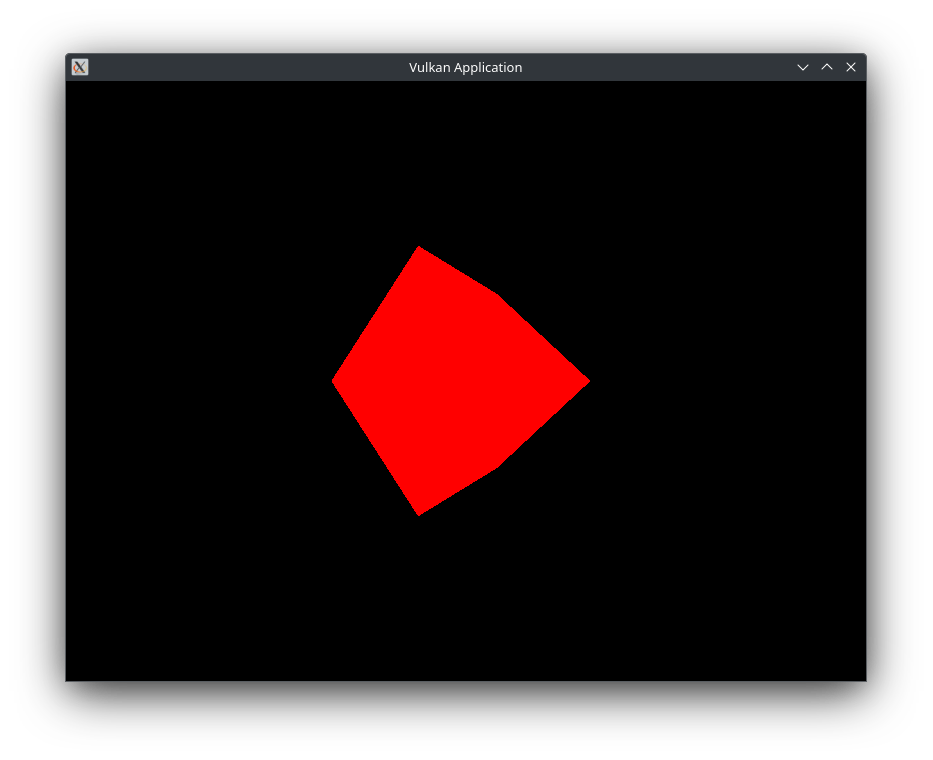
\includegraphics[width=0.8\textwidth]{images/perspective_cube.png}
	\caption{Rotated and scaled cube with perspective projection}
\end{figure}

\section{Movement}

\subsection{View Transformation}

The perspective projection matrix is a matrix that transforms the view frustum to a orthogonal frustum.
It assumes that the camera is at the origin and looks down the negative z-axis. But in video games the camera can move and rotate
freely as a player. Therefor we will have to move and rotate the camera to simulate the movement of the player.
To adjust the gameobjects accordingly to the cameras position and rotation we will have to create a view matrix.
The view matrix moves and rotates the world in a way that the camera is at the origin and looks down the negative z-axis.
In other words, the view matrix is the inverse of the camera model matrix. It will undo the movement and rotation of the camera.

The model matrix of the camera will be retrieved from a player game object via the \textit{mat4} function.
Let's calculate the invers of the model matrix. Since the camera will not be scaled, we won't apply scaling.
First we will need the inverse of the translation matrix. The inverse of a translation matrix is the negative of the translation vector.

\[
	\begin{bmatrix}
		1 & 0 & 0 & -x \\
		0 & 1 & 0 & -y \\
		0 & 0 & 1 & -z \\
		0 & 0 & 0 & 1
	\end{bmatrix}
\]

Next we will have to calculate the inverse of the rotation matrices. To better understand this we will have to look a bit deeper into the rotation matrices.
For example if we take apart the rotation matrix of the y-axis we will see that each column of the matrix describes the right, up and forward vector of the camera.

\[
	\begin{bmatrix}
		\cos(\theta)  & 0 & \sin(\theta) \\
		0             & 1 & 0            \\
		-\sin(\theta) & 0 & \cos(\theta) \\
	\end{bmatrix}
\]

The first vector describes where the vector that points to the right of the camera is pointing to.
The second vector describes where the vector that points up is pointing to.
And the third vector describes where the vector that points forward is pointing to.

If we rotate by 0 degrees we will have the following vectors:

\[
	Right:
	\begin{bmatrix}
		1 \\
		0 \\
		0 \\
	\end{bmatrix}
	Up:
	\begin{bmatrix}
		0 \\
		1 \\
		0 \\
	\end{bmatrix}
	Forward:
	\begin{bmatrix}
		0 \\
		0 \\
		1 \\
	\end{bmatrix}
\]

But if we rotate by 90 degrees we will have the following vectors:

\[
	Right:
	\begin{bmatrix}
		0  \\
		0  \\
		-1 \\
	\end{bmatrix}
	Up:
	\begin{bmatrix}
		0 \\
		1 \\
		0 \\
	\end{bmatrix}
	Forward:
	\begin{bmatrix}
		1 \\
		0 \\
		0 \\
	\end{bmatrix}
\]

Now that we know how the rotation matrix works we can calculate the inverse of the rotation matrix.
The inverse of each rotation matrix is the transposed matrix. The transposed matrix is the matrix where the rows are the columns of the original matrix.
So our inverse rotation matrix will be:

\[
	\begin{bmatrix}
		\cos(\theta) & 0 & -\sin(\theta) \\
		0            & 1 & 0             \\
		\sin(\theta) & 0 & \cos(\theta)  \\
	\end{bmatrix}
\]

When we do this for all three rotation matrices and add the translation matrix we will get the view matrix:

\[
	\fontsize{8}{12}\selectfont
	\begin{bmatrix}
		\cos(\theta_y) \cos(\theta_z) + \sin(\theta_y) \sin(\theta_x) \sin(\theta_z) & \cos(\theta_x) \sin(\theta_z) & \cos(\theta_y) \sin(\theta_x) \sin(\theta_z) - \sin(\theta_y) \cos(\theta_z) & -t_x \\
		\sin(\theta_y) \sin(\theta_x) \cos(\theta_z) - \sin(\theta_z) \cos(\theta_y) & \cos(\theta_x) \cos(\theta_z) & \sin(\theta_y) \sin(\theta_z) + \cos(\theta_y) \sin(\theta_x) \cos(\theta_z) & -t_y \\
		\sin(\theta_y) \cos(\theta_x)                                                & -\sin(\theta_x)               & \cos(\theta_y) \cos(\theta_x)                                                & -t_z \\
		0                                                                            & 0                             & 0                                                                            & 1    \\
	\end{bmatrix}
\]

The problem is that to calculate the projection view matrix we will have to multiply the projection matrix with the view matrix.
Since the view matrix will be on the right side of the multiplication we will have to transpose the matrix to multiply the x translation vector with the projection matrix's first row,
the y translation vector with the projection matrix's second row and the z translation vector with the projection matrix's third row.
The transposed view matrix will look like this:

\[
	\fontsize{8}{12}\selectfont
	\begin{bmatrix}
		\cos(\theta_y) \cos(\theta_z) + \sin(\theta_y) \sin(\theta_x) \sin(\theta_z) & \sin(\theta_y) \sin(\theta_x) \cos(\theta_z) - \sin(\theta_z) \cos(\theta_y) & \sin(\theta_y) \cos(\theta_x) & 0 \\
		\cos(\theta_x) \sin(\theta_z)                                                & \cos(\theta_x) \cos(\theta_z)                                                & -\sin(\theta_x)               & 0 \\
		\cos(\theta_y) \sin(\theta_x) \sin(\theta_z) - \sin(\theta_y) \cos(\theta_z) & \sin(\theta_y) \sin(\theta_z) + \cos(\theta_y) \sin(\theta_x) \cos(\theta_z) & \cos(\theta_y) \cos(\theta_x) & 0 \\
		-t_x                                                                         & -t_y                                                                         & -t_z                          & 1 \\
	\end{bmatrix}
\]

One final thing we will have to do is to consider that the cameras position is not always where the position of the camera game object is.
For example when we rotate the camera by 90 degrees on the y-axis and move it in the positive x direction, the camera will move in the negative z direction.
This happens because we first rotate the world and then move the camera. To consider rotation in our translation we will take the dot product of the translation vector and the rotation matrix's
right, up and forward vector. This will give us the translation vector in the world space.

For example if we rotate the camera by 90 degrees on the y-axis and move it by 1 in the positive x direction we will be at the position (0, 0, -1).
To get this result we will have to consider the right vector when moving the camera on the x axis, since the x axis is the right vector of the camera at the origin.
The new translation on the x axis will be the dot product of the right vector after rotation and the translation vector.

\[
	\begin{bmatrix}
		0  \\
		0  \\
		-1 \\
	\end{bmatrix}
	\cdot
	\begin{bmatrix}
		1 \\
		0 \\
		0 \\
	\end{bmatrix}
	=
	0
\]

This is the translation on the x axis. If you think about it this makes sense.
When we tranlate the camera we first rotate by 90 degrees to the right and then move by 1 in the positive x direction.
After rotation we actually move in the negative z direction. When we want to get back to the centre we first rotate by -90 degrees and since we
actually moved on the z axis we will not move on the x axis. When we do the the same for the y and z axis we will get the following translation vector:

\[
	\begin{bmatrix}
		0 \\
		0 \\
		1 \\
	\end{bmatrix}
\]

But because we need the inverse we will have to negate the translation vector.
So the translation vector will be the negative dot product of the translation vector and the rotation matrix's right, up and forward vector respectively.
Our final view matrix will look like this:

\[
	\fontsize{8}{12}\selectfont
	\begin{bmatrix}
		\cos(\theta_y) \cos(\theta_z) + \sin(\theta_y) \sin(\theta_x) \sin(\theta_z) & \sin(\theta_y) \sin(\theta_x) \cos(\theta_z) - \sin(\theta_z) \cos(\theta_y) & \sin(\theta_y) \cos(\theta_x)                  & 0 \\
		\cos(\theta_x) \sin(\theta_z)                                                & \cos(\theta_x) \cos(\theta_z)                                                & -\sin(\theta_x)                                & 0 \\
		\cos(\theta_y) \sin(\theta_x) \sin(\theta_z) - \sin(\theta_y) \cos(\theta_z) & \sin(\theta_y) \sin(\theta_z) + \cos(\theta_y) \sin(\theta_x) \cos(\theta_z) & \cos(\theta_y) \cos(\theta_x)                  & 0 \\
		-(rotation_{\text{right}} \cdot translation)                                 & -(rotation_{\text{up}} \cdot translation)                                    & -(rotation_{\text{forward}} \cdot translation) & 1 \\
	\end{bmatrix}
\]

In the case of our 90 degree rotation on the y-axis and the translation by 1 in the positive x direction we will get the following view matrix:

\[
	\fontsize{8}{12}\selectfont
	\begin{bmatrix}
		0  & 0 & 1  & 0 \\
		0  & 1 & 0  & 0 \\
		-1 & 0 & 0  & 0 \\
		0  & 0 & -1 & 1 \\
	\end{bmatrix}
\]

Let's start implementing the view matrix. We will add a \textit{setView} function that will take a constant position and constant rotation vector as parameters
and a new view matrix member variable. We will also add a \textit{getView} function that will return the view matrix.

\begin{lstlisting}[Language=C++]
//camera.hpp
class Camera {
public:
  ...
  void setView(const glm::vec3 &position, const glm::vec3 &rotation);
  glm::mat4 &getViewMatrix() const { return viewMatrix; }

private:
  ...
  glm::mat4 viewMatrix{1.f};
};
\end{lstlisting}

The implementation is quite simple, first we will get the sin and cos of the rotation vector and create the right, up and forward vectors.
Then we reset our view matrix and populate it with the right, up and forward vectors and the invers translation.

\begin{lstlisting}[Language=C++]
//camera.cpp
void Camera::setView(const glm::vec3 &position, const glm::vec3 &rotation) {
  const float c1 = glm::cos(rotation.y);
  const float s1 = glm::sin(rotation.y);
  const float c2 = glm::cos(rotation.x);
  const float s2 = glm::sin(rotation.x);
  const float c3 = glm::cos(rotation.z);
  const float s3 = glm::sin(rotation.z);
  const glm::vec3 u{c1 * c3 + s1 * s2 * s3, c2 * s3, c1 * s2 * s3 - s1 * c3};
  const glm::vec3 v{s1 * s2 * c3 - s3 * c1, c2 * c3, s1 * s3 + c1 * s2 * c3};
  const glm::vec3 w{s1 * c2, -s2, c1 * c2};

  viewMatrix = glm::mat4{1.f};
  viewMatrix[0][0] = u.x;
  viewMatrix[1][0] = u.y;
  viewMatrix[2][0] = u.z;
  viewMatrix[0][1] = v.x;
  viewMatrix[1][1] = v.y;
  viewMatrix[2][1] = v.z;
  viewMatrix[0][2] = w.x;
  viewMatrix[1][2] = w.y;
  viewMatrix[2][2] = w.z;
  viewMatrix[3][0] = -glm::dot(u, position);
  viewMatrix[3][1] = -glm::dot(v, position);
  viewMatrix[3][2] = -glm::dot(w, position);
};
\end{lstlisting}

Now we can simply set the view matrix in our game loop and multiply it with the projection matrix to get the projection view matrix.
We will set the view matrix to a position of (0, -0.5, 0) and a rotation of (0, -glm::radians(25.f), 0) to turn left and move up.

\begin{lstlisting}[Language=C++]
//app.cpp
...
  while (!window.shouldClose()) {
    glfwPollEvents();

    camera.setView({0.f, 0.5f, 0.5f}, {0.f, -glm::radians(25.f), 0.f});

    if (auto commandBuffer = renderSystem.beginFrame()) {
      int frameIndex = renderSystem.getFrameIndex();
      FrameInfo frameInfo{frameIndex, commandBuffer, camera,
                          descriptorSets[frameIndex]};

      GlobalUbo ubo{};
      ubo.projectionView = camera.getProjection() * camera.getView();
      uboBuffers[frameIndex]->writeToBuffer(&ubo);
      uboBuffers[frameIndex]->flush();

      renderSystem.recordCommandBuffer(commandBuffer);
      renderSystem.renderGameObjects(frameInfo, gameObjects);
      renderSystem.endRenderPass(commandBuffer);
      renderSystem.endFrame();
    }
  }
  vkDeviceWaitIdle(device.device());
\end{lstlisting}

The result should be a image where it seems like the camera has stepped up and rotated to the left.

\begin{figure}[htbp]
	\centering
	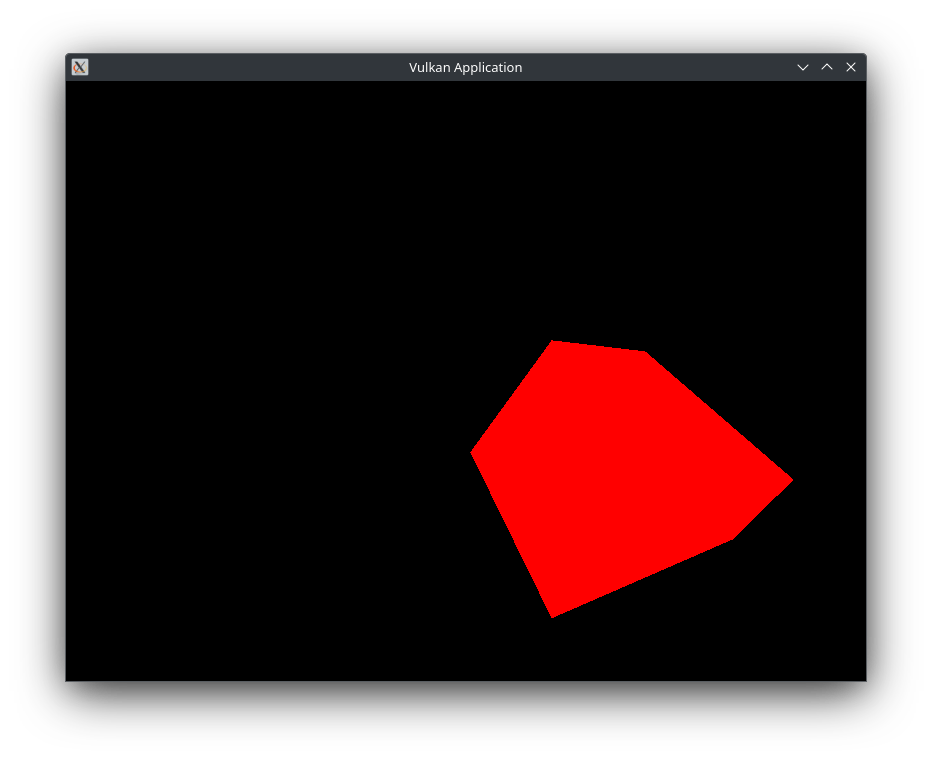
\includegraphics[width=0.8\textwidth]{images/view_transformation.png}
	\caption{Rotated cube with perspective projection and view transformation}
\end{figure} \FloatBarrier

\subsection{Moving a player}

Now that we can move the camera we can will add some input handling that will move the camera with the WASD keys and rotate it with the mouse.
Let's begin by instanciating a new game object called player.

\begin{lstlisting}[Language=C++]
//app.cpp
void App::run() {
  ...
  GameObject player = GameObject::createGameObject();

  while (!window.shouldClose()) {
    ...
}
\end{lstlisting}

Now we will need a MovementController class that will handle the movement of the player. This class will be not a core class and have a \textit{move} function that will take a game object to move and
a pointer to the \textit{GLFWwindow} object to get the inputs. It will simply check for keyboard or mouse inputs and move the player accordingly. But since the move function will be called
every frame, faster computers will move the player faster than slower computers. To fix this we will have to multiply the movement by the delta time. The delta time is the time it took to render the last frame.
So when we have a faster computer the delta time will be smaller and the player will move slower in each frame, but because the frames are rendered faster the player will move the same distance in the same time.

\begin{lstlisting}[Language=C++]
//movement_controller.hpp
#include "core/game_object.hpp"
#include <GLFW/glfw3.h>

namespace engine {

class MovementController {
public:
  void move(GLFWwindow *window, float dt, GameObject &gameObject);
};

} // namespace engine
\end{lstlisting}

Before we implement the move function we will add some key mappings in a subclass of the MovementController class called KeyMapping.
Inside the KeyMapping class we will map the GLFW key codes to a corresponding movement variable.

\begin{lstlisting}[Language=C++]
//movement_controller.hpp
class MovementController {
public:
  class KeyMapping {
  public:
    int forward = GLFW_KEY_W;
    int backward = GLFW_KEY_S;
    int left = GLFW_KEY_A;
    int right = GLFW_KEY_D;
  };
  void move(GLFWwindow *window, float dt, GameObject &gameObject);

private:
  KeyMapping keys{};
};
\end{lstlisting}

Let's go ahead and start with the translation. Later we will add the rotation.
We will first define where the forward and right vectors of the player are pointing to.
These vectors depend on the rotation of the player. To be more precise, both vectors depend on the
yaw of the player. The yaw is the rotation around the y-axis. The x-axis rotation is the pitch and the z-axis rotation is the roll.
By looking at the rotation matrix again, we can see that the forward vector is the third column of the rotation matrix
and the right vector is the first column of the rotation matrix.  We will then instanciate a translation vector and set it to zero.
Then we will check which keys are pressed and add the corresponding vectors to the translation vector.
Because we don't want the player to move slower when moving diagonally we will normalize the translation vector.
Finally we will multiply the translation vector by the delta time and add it to the position of the player.

\begin{lstlisting}[Language=C++]
//movement_controller.cpp
#include "movement_controller.hpp"
#include <glm/ext/vector_float3.hpp>

namespace engine {

void MovementController::move(GLFWwindow *window, float dt,
                              GameObject &gameObject) {
  float yaw = gameObject.transform.rotation.y;

  const glm::vec3 forwardDirection{sin(yaw), 0, cos(yaw)};
  const glm::vec3 rightDirection{forwardDirection.z, 0, -forwardDirection.x};

  glm::vec3 moveDirection{0.f};
  if (glfwGetKey(window, keys.left) == GLFW_PRESS)
    moveDirection = -rightDirection;
  if (glfwGetKey(window, keys.right) == GLFW_PRESS)
    moveDirection = rightDirection;
  if (glfwGetKey(window, keys.forward) == GLFW_PRESS)
    moveDirection = forwardDirection;
  if (glfwGetKey(window, keys.backward) == GLFW_PRESS)
    moveDirection = -forwardDirection;

  moveDirection = glm::normalize(moveDirection);
  gameObject.transform.position += moveDirection * dt;
};

} // namespace engine
\end{lstlisting}

Before we can use the MovementController class we will have instanciate it and calculate the delta time.
For the delta time we will use a high resolution clock from the \textit{chrono} extension.
Before the game loop we will save the current time with the \textit{now} function from the \textit{std::chrono::high\textunderscore resolution\textunderscore clock} class.
In the game loop we will get the new time and calculate the delta time with the \textit{duration} function from the \textit{std::chrono} extension.
This function will take the difference between the new time and the old time and convert it to a predefined time unit. We will use seconds and store the result in a float variable.
To retrieve the time as a float we will call the \textit{count} function on the result of the \textit{duration} function.
Then we will set the current time to the new time.
Finally we call the \textit{move} function of the MovementController class and pass the window, the delta time and the player game object.

\begin{lstlisting}[Language=C++]
//app.cpp
void App::run() {
  ...
  MovementController movementController{};

  GameObject player = GameObject::createGameObject();

  auto currentTime = std::chrono::high_resolution_clock::now();

  while (!window.shouldClose()) {
    glfwPollEvents();

    auto newTime = std::chrono::high_resolution_clock::now();
    float deltaTime =
        std::chrono::duration<float, std::chrono::seconds::period>(newTime -
                                                                   currentTime)
            .count();
    currentTime = newTime;

    movementController.move(window.getGLFWwindow(), deltaTime, player);
}
\end{lstlisting}

Since the \textit{move} function takes the window as a parameter we will have to add a \textit{getGLFWwindow} function to the Window class that will return the \textit{GLFWwindow} object.

\begin{lstlisting}[Language=C++]
//window.hpp
class Window {
public:
  ...
  GLFWwindow *getGLFWwindow() { return window; }
  ...
};
\end{lstlisting}

Now we can move the player with the WASD keys.

The next step is to add the rotation of the player with the mouse.
To do so we will adjust our Window class. We will set the input mode of the window to GLFW\textunderscore CURSOR\textunderscore DISABLED.
This will hide the cursor and lock it to the windows center. We will also check if raw mouse motion is supported and enable it if it is.
This last step is optional but it will give us more precise mouse movement by disabling mouse acceleration.

\begin{lstlisting}[Language=C++]
//window.cpp
...
void Window::initWindow() {
  glfwInit();

  glfwWindowHint(GLFW_CLIENT_API, GLFW_NO_API);
  glfwWindowHint(GLFW_RESIZABLE, GLFW_TRUE);

  window = glfwCreateWindow(width, height, name.c_str(), nullptr, nullptr);
  glfwSetWindowUserPointer(window, this);
  glfwSetFramebufferSizeCallback(window, framebufferResizeCallback);

  glfwSetInputMode(window, GLFW_CURSOR, GLFW_CURSOR_DISABLED);

  if (glfwRawMouseMotionSupported())
    glfwSetInputMode(window, GLFW_RAW_MOUSE_MOTION, GLFW_TRUE);
}
...
\end{lstlisting}

Now we will add the mouse movement to the \textit{move} function of the MovementController class.
To get the current mouse position we will use the \textit{glfwGetCursorPos} function. This function
takes the window and two pointers to double values as parameters. The function will then set the double values to the x and y position of the cursor.
We will need a private member variable to store the last mouse position. We will then calculate the difference between the current and the last mouse position
and add the difference to the rotation of the player.

\begin{lstlisting}[Language=C++]
//movement_controller.cpp
void MovementController::move(GLFWwindow *window, float dt,
                              GameObject &gameObject) {
  double newMouseX, newMouseY;
  glfwGetCursorPos(window, &newMouseX, &newMouseY);

  double deltaX = newMouseX - mouseX;
  double deltaY = newMouseY - mouseY;

  glm::vec3 rotateDirection{0.f};
  rotateDirection.y = deltaX;
  rotateDirection.x = -deltaY;

  gameObject.transform.rotation += rotateDirection * dt;

  mouseX = newMouseX;
  mouseY = newMouseY;
  ...
}
\end{lstlisting}

Of couse when we start the game the mouseX and mouseY variables will be uninitialized. To fix this we will add a simple boolean variable that will be set to false when the mouse position is initialized.

\begin{lstlisting}[Language=C++]
//movement_controller.cpp
void MovementController::move(GLFWwindow *window, float dt,
                              GameObject &gameObject) {
  if (firstMouse) {
    glfwGetCursorPos(window, &mouseX, &mouseY);
    firstMouse = false;
    return;
  }
  ...
}
\end{lstlisting}

With this we can move the player with the WASD keys and rotate it with the mouse.

\section{Lightning}

Currently our cube looks very flat and boring. To make it look more interesting and realistic we will add lightning.
Lightning in computer graphics is the simulation of light rays that hit an object and are reflected to the camera.
There are many different lightning models that simulate different materials and light sources.

For this tutorial we will use a combination of the Lambertian Diffuse and a basic attenuation model to simulate a matte surface with a point light source.
The Lambertian Diffuse model is a simple model that simulates a matte surface. It does not take the view direction into account and assumes that the light is reflected equally in all directions.
This is obviously not true in real life but it is a good approximation and is very cheap to calculate.

The attenuation model is a simple model that simulates the decrease of light intensity with distance.
It is based on the inverse square law that states that the intensity of light decreases with the square of the distance.

\subsection{Lambertian Diffuse}

The Lambertian Diffuse model calculates the intensity of the light that hits the surface of an object. It is based on the angle between the normal of the surface and the direction of the light.
A normal is a vector that is pointing away from the object and is perpendicular to the surface of the object. In the case of our cube the normals are pointing perpendicular to the faces of the cube.
The intensity is then calulated by evaluating the angle between the normal and the light direction with the dot product. The dot product of two vectors is the cosine of the angle between the two vectors.
The reason we use the cosine is because we want the light intensity to be at max when the light is hitting the surface directly and at zero when the light is hitting the surface at a 90 degree angle.
But because the angle will be negative when the light is hitting the surface from an angle greater than 90 degrees we will have to clamp the result to zero.

Before we begin with the lighting implementation we will have to get the normals of the cube when we load the model.
Inside of the \textit{Vertex} struct we will add a normal member variable and adjust the \textit{Vertex::getAttributeDescriptions} function accordingly.

\begin{lstlisting}[Language=C++]
//model.hpp
...
class Model {
public:
  struct Vertex {
    glm::vec3 position{};
    glm::vec3 color{1.f, 0.f, 0.f};
    glm::vec3 normal{};

    static std::vector<VkVertexInputBindingDescription>
    getBindingDescriptions();
    static std::vector<VkVertexInputAttributeDescription>
    getAttributeDescriptions();
  };
  ...
};
\end{lstlisting}

Inside the \textit{Vertex::getAttributeDescriptions} function we will add a new attribute description for the normal.

\begin{lstlisting}[Language=C++]
//model.cpp
...
attributeDescriptions.push_back(
    {2, 0, VK_FORMAT_R32G32B32_SFLOAT, offsetof(Vertex, normal)});
...
\end{lstlisting}

Luckily, gltf models already provide normals for each vertex. We will have to adjust the \textit{loadModel} function to load the normals from the gltf model.
It works basically the same as the position loading, but instead of the \textit{POSITION} accessor we will use the \textit{NORMAL} accessor.

\begin{lstlisting}[Language=C++
//model.cpp
void Model::Builder::loadModel(const std::string &filepath) {
  ...
  for (const auto &mesh : gltfModel.meshes) {
    for (const auto &primitive : mesh.primitives) {
      ...VertexBuffer loading...
      const auto &normalAccessor =
          gltfModel.accessors[primitive.attributes.at("NORMAL")];
      const auto &normalBufferView =
          gltfModel.bufferViews[normalAccessor.bufferView];
      const auto &normalBuffer = gltfModel.buffers[normalBufferView.buffer];
      const float *normalData = reinterpret_cast<const float *>(
          &normalBuffer
               .data[normalBufferView.byteOffset + normalAccessor.byteOffset]);

      for (size_t i = 0; i < vertexAccessor.count; i++) {
        Vertex vertex{};
        vertex.position = {vertexData[i * 3], vertexData[i * 3 + 1],
                           vertexData[i * 3 + 2]};
        vertex.normal = {normalData[i * 3], normalData[i * 3 + 1],
                         normalData[i * 3 + 2]};
        vertices.push_back(vertex);
      }
      ...IndexBuffer loading...
    }
  }
}
\end{lstlisting}

Great now that we have the normals we also have to create a normal matrix. Just as the model matrix transforms the vertices of the object to the world space,
the normal matrix transforms the normals of the object to the world space. Okay but why not use the model matrix for the normals? The reason is best explained with an example.
Let's imagine a triangle where the vertices are at the positions (1, 1, 0), (-1, 1, 0) and (0, 0, 1).
The normal of this triangle can be calculated by taking the cross product of two edges of the triangle.

The first triangle edge is the vector from (1,1,0) to (-1,1,0) which is (-2, 0, 0).
The second triangle edge is the vector from (1,1,0) to (0,0,1) which is (-1, -1, 1).

The cross product of these two vectors is the normal of the triangle which is (0, -2, -2) or (0, 2, 2) depending on the order of the cross product.
This normal is already provided by the gltf model. But what happens when we scale the triangle by 2 in the z direction, effectively transforming the third vertex to (0, 0, 2)?

Vector 1 is still (-2, 0, 0) and vector 2 will turn into (-1, -1, 2). The cross product of these two vectors is now (0, -4, -2) or (0, 4, 2).
Because of the way the cross product works, each axis of the normal will be scaled by the scale factor except for the axis that we scaled the object in.
So when we scale the object on the z axis it will scale the x and y axis of the normal by the scale factor. This is something that the model matrix does not do.
The model matrix scales the object by the same factor by the scale factor for the corresponding axis.

Since we want to scale the other axes of the normal by the scale factor we can simply multiply the scaled axis by the inverse of the scale factor.
So when we scale the object by 2 in the z direction we will can multiply the z axis of the normal by 0.5 to get the correct normal.
This is correct since we only care about the direction of the normal and not the length of the normal.

The reason the y axis of the example normal is scaled by 2 is because when we scale the object by 2 in the z direction the triangle flattens, what means that the normal will point further up then before.
This can be perfectly seen when we draw both triangles on a piece of paper and draw the normals of the triangles.

//Add images here

So the normal matrix will be the same as the model matrix but with the inverse scale factors and without the translation.
We cut out the translation because it does not affect the direction of the normal.
Let's add a \texit{normalMatrix} function to the Transform struct that will return the normal matrix.

\begin{lstlisting}[Language=C++]
//game_object.cpp

glm::mat4 Transform::normalMatrix() {
  const float c1 = glm::cos(rotation.y);
  const float s1 = glm::sin(rotation.y);
  const float c2 = glm::cos(rotation.x);
  const float s2 = glm::sin(rotation.x);
  const float c3 = glm::cos(rotation.z);
  const float s3 = glm::sin(rotation.z);
  const glm::vec3 invScale = 1.f / scale;

  return glm::mat4{
      {
          invScale.x * (c1 * c3 + s1 * s2 * s3),
          invScale.x * c2 * s3,
          invScale.x * (c1 * s2 * s3 - s1 * c3),
          0.f,
      },
      {
          invScale.y * (s1 * s2 * c3 - s3 * c1),
          invScale.y * c2 * c3,
          invScale.y * (s1 * s3 + c1 * s2 * c3),
          0.f,
      },
      {
          invScale.z * s1 * c2,
          invScale.z * -s2,
          invScale.z * c1 * c2,
          0.f,
      },
      {0.f, 0.f, 0.f, 1.f},
  };
}

\end{lstlisting}

Now we will need to add a member variable to the PushConstantData struct that will hold the normal matrix.

\begin{lstlisting}[Language=C++]
//render_system.cpp

struct PushConstantData {
  glm::mat4 modelMatrix;
  glm::mat4 normalMatrix;
};
\end{lstlisting}

Further more we will have to populate the normal matrix in the \textit{renderGameObjects} function.

\begin{lstlisting}[Language=C++]
//render_system.cpp

void RenderSystem::renderGameObjects(FrameInfo &frameInfo,
                                     std::vector<GameObject> &gameObjects) {
  pipeline->bind(frameInfo.commandBuffer);

  vkCmdBindDescriptorSets(frameInfo.commandBuffer,
                          VK_PIPELINE_BIND_POINT_GRAPHICS, pipelineLayout, 0, 1,
                          &frameInfo.descriptorSet, 0, nullptr);

  for (GameObject &gameObject : gameObjects) {
    PushConstantData push{};
    push.modelMatrix = gameObject.transform.mat4();
    push.normalMatrix = gameObject.transform.normalMatrix();

    vkCmdPushConstants(frameInfo.commandBuffer, pipelineLayout,
                       VK_SHADER_STAGE_VERTEX_BIT, 0, sizeof(PushConstantData),
                       &push);

    gameObject.model->bind(frameInfo.commandBuffer);
    gameObject.model->draw(frameInfo.commandBuffer);
  }
}
\end{lstlisting}

Now we can access the normal matrix in the vertex shader. We will add a new member variable to the PushConstant struct that will hold the normal matrix.
We will also add a new in variable to the vertex shader that will hold the normal.

\begin{lstlisting}[Language=C++]
//shader.vert

layout(location = 0) in vec3 inPosition;
layout(location = 1) in vec3 inColor;
layout(location = 2) in vec3 inNormal;

layout(location = 0) out vec3 fragColor;

layout(push_constant) uniform Push {
  mat4 modelMatrix;
  mat4 normalMatrix;
} push;
...
\end{lstlisting}

We're finished with the normals and can focus on the lambertian diffuse model.
Like mentioned before the lambertian diffuse model calculates the intensity of the light that hits the surface of an object.
The intensity is calculated by evaluating the angle between the normal of the surface and the direction of the light using the dot product.
The dot product of two vectors is the cosine of the angle between the two vectors.
Since we need the direction of the light we will have to provide the position of the light source.
We can not provide it as a push constant, because it does not contain enough space for another vec3.
Remember that the push constant is limited to 128 bytes, aka 32 floats, aka two 4x4 matrices.
That's why we will provide it via the uniform buffer and also provide the color of the light source and an ambient light color.

\begin{lstlisting}[Language=C++]
//app.cpp

struct GlobalUbo {
  glm::mat4 projectionView{1.f};
  glm::vec4 ambientLightColor{1.f, 1.f, 1.f, .02f};
  glm::vec3 lightPosition{-1.f};
  alignas(16) glm::vec4 lightColor{1.f};
};
...
\end{lstlisting}

Take into consideration that each object in the uniform buffer will be automatically aligned to 16 bytes. This means, that
the shader can only access objects on a 16 byte boundary. This is why we have to add the \textit{alignas(16)} attribute to the \textit{lightColor} member variable.
Without this attribute the \textit{lightColor} member would begin at the 92th byte of the uniform buffer, because the mat4, vec3 and vec4 objects are 92 bytes in total.
Because of the alignment rules, the shader would access the \textit{lightColor} member at the 96th byte, which would cut out the first 4 bytes of the \textit{lightColor} member.
This would result in a wrong value for the \textit{lightColor} member.
But the \textit{alignas(16)} attribute will align the \textit{lightColor} member to the 96th byte, so the shader can access the \textit{lightColor} member correctly.

For the light intensity, we will first have to calculate the world position of the vertex and its normals.
This means we will have to multiply the vertex position with the model matrix and the normal with the normal matrix.
We will then calculate the direction of the light by subtracting the world position of the vertex from the world position of the light.
The light position is provided as a vec3, so we will have to convert the world position of the vertex to a vec3 by dividing the world position by accessing its x, y and z components.

Before we can calculate the intensity we will have to normalize the normal and the light direction. We do this, to simplify the calculation of the dot product.
The full formula for the dot product is:

\[
	\vec{a} \cdot \vec{b} = \left\| \vec{a} \right\| \left\| \vec{b} \right\| \cos(\theta)
\]

Where $\vec{a}$ and $\vec{b}$ are the two vectors and $\theta$ is the angle between the two vectors.
When we normalize the vectors the length of the vectors will be 1 and the formula simplifies to:

\[
	\vec{a} \cdot \vec{b} = \cos(\theta)
\]

This is the reason why we normalize the vectors before calculating the dot product.
The intensity is then calculated by taking the dot product of the normal and the light direction.
Since the dot product can be negative when the normal is facing away from the light, we will have to clamp the result to zero.
We will also transform the normal matrix to a mat3 matrix, so that we can multiply it with the vec3 normal.

\begin{lstlisting}[Language=C++]
//shader.vert
...
void main() {
  vec4 worldPosition = push.modelMatrix * vec4(inPosition, 1.0);
  vec3 normalWorldSpace = normalize(mat3(push.normalMatrix) * inNormal);
  vec3 directionToLight = normalize(ubo.lightPosition - worldPosition.xyz);

  float lightIntensity = max(dot(normalWorldSpace, directionToLight), 0);
}
\end{lstlisting}

We will then multiply the light and ambient colors x, y and z components with it's w component, which is the
opacity or alpha value of the color. This is done to change the light and ambient color intensity with the alpha value.

\begin{lstlisting}[Language=C++]
//shader.vert
...
void main() {
  ...
  vec3 lightColor = ubo.lightColor.xyz * ubo.lightColor.w;
  vec3 ambientLight = ubo.ambientLightColor.xyz * ubo.ambientLightColor.w;
}
\end{lstlisting}

Now we can get the diffuse color by multiplying the light intensity with the light color.
With the diffuse color we can calculate the final color by adding the diffuse color to the ambient light color and multiply the result with the vertex color.
We should also not forget to pass the final color to the fragment shader and multiply the world position with the projection view matrix
to set the gl\textunderscore Position.

\begin{lstlisting}[Language=C++]
//shader.vert
...
void main() {
  ...
  vec3 diffuseLight = lightColor * lightIntensity;

  fragColor = inColor * (ambientLight + diffuseLight);
  gl_Position = ubo.projectionMatrix * worldPosition;
}
\end{lstlisting}

With all of that done we should see a cube that is lit by a light source.

\subsection{Attenuation}

The attenuation model simulates the decrease of light intensity with distance.
This simulation is based on the inverse square law that states that the intensity of light decreases with the square of the distance.
The attenuation model is based on three factors: the constant factor, the linear factor and the quadratic factor.

The constant factor is a constant value that is added to the attenuation model.
It is usually set to 1 to avoid division by zero and to fully illuminate the object when the light source is close to the object.

The linear factor is a value that is multiplied with the distance between the light source and the object.
It is used to simulate a linear decrease of light intensity with distance. The linear factor is usually set to a value between 0 and 1.

The quadratic factor is a value that is multiplied with the square of the distance between the light source and the object.
It is used to simulate a quadratic decrease of light intensity with distance. The quadratic factor is usually set to a value between 0 and 1.

So the attenuation model is calculated by the following formula:

\[
	\frac{lightIntensity}{constant + linear \cdot distance + quadratic \cdot distance^2}
\]

For the constant factor we will use 1, for the linear and quadratic factor we will use 0.2 to simulate a medium decrease of light intensity with distance.
We have to calculate the distance between the light source and the object. We can do this with the length function that calculates the length of a vector.
Because we normalized the light direction vector the lenght will be alway 1. So we have to undop the normalization and normalize the vector later when we have to.

\begin{lstlisting}[Language=C++]
//shader.vert
...
void main() {
  vec4 worldPosition = push.modelMatrix * vec4(inPosition, 1.0);
  vec3 normalWorldSpace = normalize(mat3(push.normalMatrix) * inNormal);

  vec3 directionToLight = ubo.lightPosition - worldPosition.xyz;
  float distanceToLight = length(directionToLight);

  float lightIntensity = max(dot(normalWorldSpace, normalize(directionToLight)), 0);
  float attenuation = lightIntensity / (1.0 + 0.2 * distanceToLight + 0.2 * distanceToLight * distanceToLight);
  ...
}
\end{lstlisting}

You can now see the light intensity decrease with distance by changing the light position.

\subsection{Per Fragment Lightning}

Currently we handle the lightning per vertex. This means that the light intensity is calculated for each vertex and the color of the vertex is interpolated between the vertices.
This is a simple and fast way to calculate lightning but it can lead to flat looking objects with sharp transitions between the colors.
To counteract this we can calculate the light intensity per fragment. This requires us to interpolate the normals and fragment positions between the vertices and calculate the light intensity in the fragment shader.
To interpolate the normals we will have to pass the normals to the rasterizer. Just as the color and position,
the normals are interpolated between the vertices inside the rasterizer and further pushed to the fragment shader.
Inside of the fragment shader we will then calculate the light intensity and the final color.

Let's first adjust the vertex shader. We will only calculate the world position and the world normal, pass them further, apply the projection matrix to the world position and pass the color to the fragment shader.

\begin{lstlisting}[Language=C++]
//shader.vert
...
layout(location = 0) out vec3 fragColor;
layout(location = 1) out vec3 fragPositionWorld;
layout(location = 2) out vec3 fragNormalWorld;

void main() {
  vec4 worldPosition = push.modelMatrix * vec4(inPosition, 1.0);
  fragNormalWorld = normalize(mat3(push.normalMatrix) * inNormal);
  fragPositionWorld = worldPosition.xyz;

  gl_Position = ubo.projectionMatrix * worldPosition;
  fragColor = inColor;
}
\end{lstlisting}

Inside of the fragment shader we will calculate the light intensity and the final color.
There are two condition that we have to take into account. The normals are interpolated between the vertices and result in normals that are not normalized.
This means that we will need to normalize the normals before calculating the light intensity.
The second condition is that we will need the data from the uniform buffer. But when creating the descripor set layout we defined the binding only for the vertex buffer.
We will have to change the binding to include the fragment shader as well.

\begin{lstlisting}[Language=C++]
//app.cpp
...
auto descriptorSetLayout =
    DescriptorSetLayout::Builder(device)
        .addBinding(0, VK_DESCRIPTOR_TYPE_UNIFORM_BUFFER,
                    VK_SHADER_STAGE_VERTEX_BIT | VK_SHADER_STAGE_FRAGMENT_BIT)
        .build();
...
\end{lstlisting}

\begin{lstlisting}[Language=C++]
//shader.frag
#version 460

layout(location = 0) in vec3 fragColor;
layout(location = 1) in vec3 fragPositionWorld;
layout(location = 2) in vec3 fragNormalWorld;

layout(location = 0) out vec4 outColor;

layout(set = 0, binding = 0) uniform GlobalUbo{
  mat4 projectionMatrix;
  vec4 ambientLightColor;
  vec3 lightPosition;
  vec4 lightColor;
} ubo;

void main() {
  vec3 directionToLight = ubo.lightPosition - fragPositionWorld;
  float distanceToLight = length(directionToLight);

  float lightIntensity = max(dot(normalize(fragNormalWorld), normalize(directionToLight)), 0);
  float attenuation = lightIntensity / (1.0 + 0.2 * distanceToLight + 0.2 * distanceToLight * distanceToLight);

  vec3 lightColor = ubo.lightColor.xyz * ubo.lightColor.w;
  vec3 diffuseLight = lightColor * attenuation;

  vec3 ambientLight = ubo.ambientLightColor.xyz * ubo.ambientLightColor.w;
  outColor = vec4(fragColor * (ambientLight + diffuseLight), 1.0f);
}
\end{lstlisting}

This should result in a more realistic looking cube.
To see the effect even better we can add a second cube as a floor.

\begin{lstlisting}[Language=C++]
//app.cpp
...
  GameObject floor = GameObject::createGameObject();
  floor.model = cubeModel;
  floor.transform.position = {0.f, -1.f, 0.f};
  floor.transform.scale = {10.f, 0.1f, 10.f};
  gameObjects.push_back(std::move(floor));
...
\end{lstlisting}

Let's compile and run the application.

\begin{figure}[htbp]
	\centering
	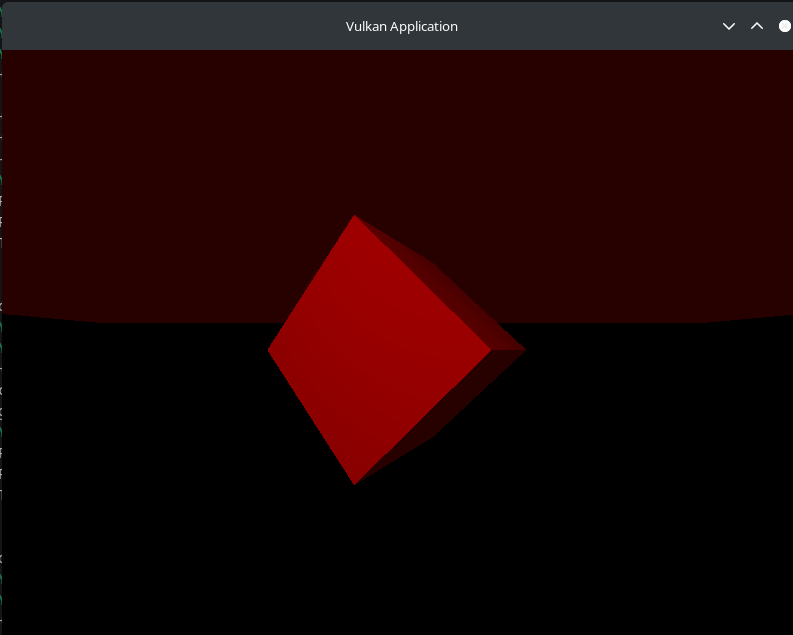
\includegraphics[width=0.8\textwidth]{images/floor_error.png}
	\caption{Per fragment lightning}
\end{figure} \FloatBarrier

Whoops I forgot that the y axis is flipped in the Vulkan coordinate system. You know what. The flipped y axis is quite annoying and unintuitive.
It's is also not the standard in computer graphics but rather originates from a more accurate representation of the graphics hardware, because
most drivers use a top left origin for the framebuffer. But because we are using Vulkan we can change the y axis to the standard bottom left origin.
This will unflip the y axis and make the coordinate system more intuitive.

To do so we will have to change the viewport by setting the y value to the height of the swapchains extent. This will set the origin of the viewport to the bottom left corner of the window.
Then we will also have to negate the viewports height since it's y axis is pointing down and we want it to point up.

\begin{lstlisting}[Language=C++]
//render_system.cpp
...
  VkViewport viewport = {};
  viewport.x = 0;
  viewport.y = static_cast<float>(swapChain->extent().height);
  viewport.width = static_cast<float>(swapChain->extent().width);
  viewport.height = -static_cast<float>(swapChain->extent().height);
  viewport.minDepth = 0.0f;
  viewport.maxDepth = 1.0f;
  vkCmdSetViewport(commandBuffer, 0, 1, &viewport);
...
\end{lstlisting}

When compiling and running the application we should see the cube and the floor as expected, but the camera movement is inverted.
Let's fix this by uninverting the x axis of the mouse movement.

\begin{lstlisting}[Language=C++]
//movement_controller.cpp
...
glm::vec3 rotateDirection{0.f};
rotateDirection.y = deltaX;
rotateDirection.x = deltaY;
...
\end{lstlisting}

Perfect. Now we have a cube that is lit by a light source and a floor that is also lit by the light source.

\chapter{Rigid Body Physics}

Rigid Bodies are non-deformable objects that are used in physics simulations to simulate the movement of objects.
It handles the application of forces, the calculation of the velocity and updates the position of the parent object.
The rigid body physics engine will be a core class that will be used by the game objects to simulate gravity, forces and collisions.

\section{Rigid Body}

For now we will only implement the rigid body physics engine and add gravity to the game objects.
Let's create a new class called RigidBody3D that will have a velocity vector and a gravity float value.
Additionally we will add a \textit{applyGravity} function that will apply the gravity to the velocity vector,
a \textit{update} function that will update the position of the parent object and a \textit{resetVelocity}
function that will reset the velocity vector.

\begin{lstlisting}[Language=C++]
//rigidbody3d.hpp
#include <glm/ext/vector_float3.hpp>
namespace engine {

class RigidBody3D {
public:
  float gravity = 1.f;

  glm::vec3 velocity{0.f};

  void applyGravity(const float deltaTime);
  void update(glm::vec3 &position);
  void resetVelocity();
};
} // namespace engine
\end{lstlisting}

In the implementation of the \textit{applyGravity} function we will multiply the gravity value by the delta time
and subtract it to the y component of the velocity vector. The update function will then add the velocity vector to the position vector.

\begin{lstlisting}[Language=C++]
#include "rigidbody3d.hpp"

namespace engine {
void RigidBody3D::applyGravity(const float deltaTime) {
  velocity.y -= gravity * deltaTime;
}

void RigidBody3D::update(glm::vec3 &position) { position += velocity; }

void RigidBody3D::resetVelocity() { velocity = glm::vec3{0.f}; }
} // namespace engine
\end{lstlisting}

Let's also create a Player class that inherits from the GameObject class and adds a RigidBody3D object to the player.
Additionally it will provide a boolean flag that will indicate if the player can jump.

\begin{lstlisting}[Language=C++]
//player.hpp
#pragma once
#include "core/rigidbody3d.hpp"
#include <glm/fwd.hpp>
#include <vector>

namespace engine {

class Player : public GameObject {
public:
  bool canJump = false;

  RigidBody3D rigidBody{};
};

} // namespace engine
\end{lstlisting}

Let's call the \textit{applyGravity} function and the \textit{update} function in our game loop.

\begin{lstlisting}[Language=C++]
//app.cpp
void App::run() {
  ...
  Player player{};

  while (!window.shouldClose()) {
      ...
      player.rigidBody.applyGravity(deltaTime);
      player.rigidBody.update(player.transform.position);
      ...
    }
}
\end{lstlisting}

When you run the application you should see the player fall down but not stop at the floor.
So let's check collisions in the next section.

\section{Collision Detection}

There are many different ways to detect collisions between objects. Since we are working with cubes we will use the AABB collision detection.
AABB stands for Axis Aligned Bounding Box and is a simple collision detection algorithm that uses the axis aligned bounding boxes of the objects to detect collisions.
A bounding box is the hit box. As long as both bounding boxes are parallel to the coordinate axis we can use the AABB collision detection.

The AABB collision detection works by checking if the bounding boxes of two objects overlap. We can do so by comparing the minimum and maximum values of the bounding boxes.
For example, in 2D we can check if either the first objects minimum is greater than the other objects maximum or the first objects maximum is smaller than the other objects minimum.

Let's add a new File called \textit{collision.hpp} that will contain a CollisionBox3D struct, that will hold the minimum and maximum values of the bounding box.

\begin{lstlisting}[Language=C++]
#pragma once
#include "core/game_object.hpp"
#include <glm/glm.hpp>

namespace engine {
struct CollisionBox3D {
glm::vec3 min;
glm::vec3 max;
};
} // namespace engine
\end{lstlisting}

Let's also add a BoxCollider class that will have a CollisionBox3D object and a \textit{checkCollision} function that will check if two BoxCollider objects overlap.
If the bounding boxes overlap the function will return true, otherwise it will return false. If they overlap we will resolve the collision
and return a Collision3D object that will hold the direction and length of the collision and also a boolean flag to indicate the collision state.
We will also add some contructors to the BoxCollider class. These will set the minimum and maximum values of the bounding box.

\begin{lstlisting}[Language=C++]
//collision.hpp
namespace engine {
...
class Collision3D {
public:
bool isColliding;

glm::vec3 direction;
float length;
};

class BoxCollider {
public:
BoxCollider() { BoxCollider(Transform()); }
BoxCollider(const Transform &transform);

bool checkCollision(const CollisionBox3D &other);
Collision3D resolveCollision(const CollisionBox3D &other);

CollisionBox3D collisionBox;
};
} // namespace engine
\end{lstlisting}

Let's implement the BoxCollider class. We will first implement the constructors.
When we add a transform to the constructor we will set the collision boxes minimum to the position of the transform and
the maximum to the position of the transform plus the scale of the transform. If we don't provide a transform we will assume the scale to be 1 aka
we assume it to be a unit cube and use an empty transform for the construction.

\begin{lstlisting}[Language=C++]
#include "collision.hpp"
#include "core/game_object.hpp"
#include <algorithm>
#include <glm/fwd.hpp>

namespace engine {

BoxCollider::BoxCollider(const Transform &transform) {
collisionBox.min = transform.position;
collisionBox.max = transform.position + transform.scale;
}

} // namespace engine
\end{lstlisting}

The \textit{checkCollision} function will check if the bounding boxes overlap. We will do so by checking if the minimum of the first bounding box is greater than the maximum of the second bounding box
or if the maximum of the first bounding box is smaller than the minimum of the second bounding box. If one of these conditions is true we will return false, otherwise we will return true.

\begin{lstlisting}[Language=C++]
namepsace engine {
...
bool BoxCollider::checkCollision(const CollisionBox3D &other) {
return collisionBox.min.x < other.max.x && collisionBox.max.x > other.min.x &&
       collisionBox.min.y < other.max.y && collisionBox.max.y > other.min.y &&
       collisionBox.min.z < other.max.z && collisionBox.max.z > other.min.z;
}
} // namespace engine
\end{lstlisting}

Next the \textit{resolveCollision} function will resolve the collision. We will first calculate the overlap length of the bounding boxes for each axis.
To get the overlap length we will subtract the smaller maximum value from the larger minimum value. Then we can calculate the direction of the collision by
checking for the smallest overlap length. Finally we will have to negate the direction if the minimum of the first bounding box is smaller than the minimum of the second bounding box.

\begin{lstlisting}[Language=C++]
namespace engine {
...
Collision3D BoxCollider::resolveCollision(const CollisionBox3D &other) {
Collision3D collision;
collision.isColliding = false;

if (checkCollision(other)) {
		collision.isColliding = true;

		float xOverlap = std::min(collisionBox.max.x, other.max.x) -
		std::max(collisionBox.min.x, other.min.x);
		float yOverlap = std::min(collisionBox.max.y, other.max.y) -
		std::max(collisionBox.min.y, other.min.y);
		float zOverlap = std::min(collisionBox.max.z, other.max.z) -
		std::max(collisionBox.min.z, other.min.z);

		if (xOverlap < yOverlap && xOverlap < zOverlap) {
				collision.direction = {1, 0, 0};
				collision.length = xOverlap;
			} else if (yOverlap < xOverlap && yOverlap < zOverlap) {
				collision.direction = {0, 1, 0};
				collision.length = yOverlap;
			} else {
				collision.direction = {0, 0, 1};
				collision.length = zOverlap;
			}

		if (collisionBox.min.x < other.min.x)
		collision.direction.x *= -1;
		if (collisionBox.min.y < other.min.y)
		collision.direction.y *= -1;
		if (collisionBox.min.z < other.min.z)
		collision.direction.z *= -1;
	}
return collision;
} // namespace engine
\end{lstlisting}

Now we can add a BoxCollider object to the Player class. But the floor also needs a BoxCollider object.
So let's add header class called block.hpp. It will deefine a Block class that will inherit from the GameObject class and add a BoxCollider object to the block.
Additionally we will add a BlockType struct that will hold the type of the block as a uint8_t and a return it when we call the operator \textit{int()}.
It will also define static BlockType objects for the different block types and overwrites the \textit{operator=} to set the type of the block.
The block class will also have 2 constructors. One that will use the position of the block and set the minimum and maximum values of the bounding box to the position and the position plus 1.
The other constructor will use a transform object and pass it to the BoxCollider constructor.

\begin{lstlisting}[Language=C++]
//block.hpp
#pragma once
#include "collision.hpp"
#include "core/game_object.hpp"
#include <cstdint>
#include <sys/types.h>

namespace engine {
struct BlockType {
  const static uint8_t Air = 0;
  const static uint8_t Stone = 1;

  uint8_t type;

  operator int() const { return type; }
  BlockType &operator=(const int &other) {
    type = other;
    return *this;
  }
};

class Block : public GameObject {
public:
  Block(glm::vec3 position) : GameObject() {
    transform.position = position;
    collider.collisionBox.min = position;
    collider.collisionBox.max = position + glm::vec3(1.0f);
  }
  Block(Transform transform) : GameObject() {
    transform.position = transform.position;
    collider = BoxCollider{transform};
  }

  BlockType type;
  BoxCollider collider;
};

} // namespace engine
\end{lstlisting}

Great let's rewrite the app.cpp file to include the new classes.

\section{Collision Handling}

\printbibliography

\end{document}
\end{document}
\end{document}
